\documentclass[12pt]{vuthesis}
\usepackage[T1]{fontenc}
\usepackage{mathptmx}
\usepackage[scaled=0.92]{helvet}
\usepackage{courier}
\usepackage{ifpdf}

\ifpdf
\usepackage[pdftex]{graphicx}
\graphicspath{{figures/}}
\else
\usepackage{graphicx}
\graphicspath{{figures/}}
\fi

\usepackage[numbers]{natbib}
\usepackage{bibentry}

\newcommand{\ignore}[1]{}
\newcommand{\nobibentry}[1]{{\let\nocite\ignore\bibentry{#1}}}
% apsrev entries in the text need definitions of these commands
\newcommand{\bibfnamefont}[1]{#1}
\newcommand{\bibnamefont}[1]{#1}

\usepackage{float}
\usepackage{amsfonts,amssymb,amsmath, amsthm}
\usepackage{tabulary}
\usepackage{setspace}
\setlength\tymin{30pt}
\setlength\tymax{\linewidth}
\usepackage[font={bf,sf}]{caption}
%\usepackage[format=hang,margin=10pt,font={bf,sf}]{caption}
\usepackage{url}
\usepackage[usenames,dvipsnames]{color}
\usepackage{colortbl}
\usepackage{textcomp}
\usepackage{relsize,fancyvrb}
%\usepackage[ruled,noline]{algorithm2e}
\usepackage{subfigure}
%\usepackage{subcaption}
\usepackage{rotating}
\usepackage{tocvsec2}
\usepackage{chngcntr}

\usepackage{algorithm}
\usepackage{algorithmic}
% algorithm & algorithmic  OR  algorithm, algorithmcx, & algpseudocode
%\usepackage{algorithm}
%\usepackage{algorithmicx}
%\usepackage{algpseudocode}
\usepackage{tabularx,booktabs,lscape,rotating,multirow}
\usepackage{listings}

\usepackage{acronym}
%\usepackage[acronym,toc]{glossaries}

\ifpdf
\usepackage[pdftex,linktocpage,bookmarks,colorlinks,linkcolor=blue,urlcolor=blue,citecolor=blue,naturalnames]{hyperref}
\else
\usepackage[dvips,linktocpage,bookmarks,colorlinks,linkcolor=blue,urlcolor=blue,citecolor=blue,naturalnames]{hyperref}
\fi

\newcounter{num}
\newenvironment{NumList}
{\begin{list}
{\arabic{num}. }
{\usecounter{num}
\setlength{\topsep}{1pt}
\setlength{\parsep}{0pt}
\setlength{\itemsep}{1pt}
\setlength{\parskip}{0pt}
\setlength{\labelsep}{1pt}
\setlength{\itemindent}{0pt}
\setlength{\leftmargin}{8pt}}}
{\end{list}
\vspace{2pt}
}

\floatstyle{boxed}
\counterwithout{figure}{chapter}
\counterwithout{table}{chapter}
\counterwithout{equation}{chapter}
\renewcommand \thesection{\arabic{chapter}.\arabic{section}}
\DeclareMathAlphabet{\mathpzc}{OT1}{pzc}{m}{it}

\usepackage{listings}
\lstdefinestyle{customc}{
  belowcaptionskip=1\baselineskip,
  breaklines=true,
  frame=L,
  xleftmargin=\parindent,
  language=C,
  showstringspaces=false,
  basicstyle=\footnotesize\ttfamily,
  keywordstyle=\bfseries\color{green!40!black},
  commentstyle=\itshape\color{purple!40!black},
  identifierstyle=\color{blue},
  stringstyle=\color{orange},
}

\lstdefinestyle{customasm}{
  belowcaptionskip=1\baselineskip,
  frame=L,
  xleftmargin=\parindent,
  language=[x86masm]Assembler,
  basicstyle=\footnotesize\ttfamily,
  commentstyle=\itshape\color{purple!40!black},
}

\lstset{escapechar=@,style=customc}

\usepackage{minted}

\usepackage[toc,page]{appendix}

%\newtheorem{theorem}{Theorem}[section]
%\newtheorem{lemma}[theorem]{Lemma}
%\newtheorem{proposition}[theorem]{Proposition}
%\newtheorem{corollary}[theorem]{Corollary}

%\newenvironment{proof}[1][Proof]{\begin{trivlist}
%\item[\hskip \labelsep {\bfseries #1}]}{\end{trivlist}}
\newenvironment{definition}[1][Definition]{\begin{trivlist}
\item[\hskip \labelsep {\bfseries #1}]}{\end{trivlist}}
%\newenvironment{example}[1][Example]{\begin{trivlist}
%\item[\hskip \labelsep {\bfseries #1}]}{\end{trivlist}}
%\newenvironment{remark}[1][Remark]{\begin{trivlist}
%\item[\hskip \labelsep {\bfseries #1}]}{\end{trivlist}}

%\newcommand{\qed}{\nobreak \ifvmode \relax \else
%      \ifdim\lastskip<1.5em \hskip-\lastskip
%      \hskip1.5em plus0em minus0.5em \fi \nobreak
%      \vrule height0.75em width0.5em depth0.25em\fi}

\def\fulltool/{\textbf{P}recise \textbf{N}etwork \textbf{P}erformance \textbf{P}rediction}
\def\shorttool/{$PNP^2$}

\begin{document}
	
\nobibliography*

\title{Network Performance Analysis and Management for Cyber-Physical Systems and Their Applications}
\author{William A. Emfinger}
\submitdate{December, 2015}
\principaladviser{Dr. Gabor Karsai}
\academicarea{Electrical Engineering}

\beforepreface
%\input{copyright}



The DARPA System F6, AFRL RESOS, and AFRL SURE Projects supported
this work. Any opinions, findings, and conclusions or recommendations expressed
in this material are those of the authors and do not reflect the views of
DARPA or AFRL. 

%\input{Acronyms}
\afterpreface

\lstdefinestyle{XML}{basicstyle=\footnotesize, tabsize=2, captionpos=b, breaklines=true, firstnumber=last, keywordstyle=\color{Black}, identifierstyle=\color{Black}, stringstyle=\color{Blue}, commentstyle=\color{Gray}, tagstyle=\color{BrickRed}, markfirstintag=true}

% $Id: intro.tex 3799 2013-10-14 16:13:38Z emfinger $
\chapter{Introduction}
\label{ch:intro}

%%%%%%%%%%%%%%%%%%%%%%%%%%%%%%%%%%%%%%%%%%%%%%%%%%%%%%%%%%%%%%%%%%%%%%%%%%%%%%%%%%%
%%%%%%%%%%%%%%%%%%%%%%%%%%%%%%%%%%%%%%%%%%%%%%%%%%%%%%%%%%%%%%%%%%%%%%%%%%%%%%%%%%%
%%%%%%%%%%%%%%%%%%%%%%%%%%%%%%%%%%%%%%%%%%%%%%%%%%%%%%%%%%%%%%%%%%%%%%%%%%%%%%%%%%%
%%%%%%%%%%%%%%%%%%%%%%%%%%%%%%%%%%%%%%%%%%%%%%%%%%%%%%%%%%%%%%%%%%%%%%%%%%%%%%%%%%%
%%%%%%%%%%%%%%%%%%%%%%%%%%%%%%%%%%%%%%%%%%%%%%%%%%%%%%%%%%%%%%%%%%%%%%%%%%%%%%%%%%%
\section{Motivation}
\label{sec:motivation}

\iffalse
\begin{itemize}
	\item What's needed in system design today?
	\begin{itemize}
		\item need for verification (high criticality / hard to access)
		\item need for precision (low resources, predictability)
		\item need for adaptation at run-time
		\item need for analyzable model of run-time adaptation
	\end{itemize}
	\item types of systems:
	\begin{itemize}
		\item clusters of satellites (fractionated satellite platform, research platforms, infrastructure)
		\item unmanned aerial vehicles (UAVs: search and rescue, military assistance, etc.)
		\item unmanned underwater vehicles (UUVs: search and rescue, research, etc.)
		\item autonomous vehicles (cars and the infrastructure)
		\item CCTV infrastructure
	\end{itemize}
	\item mention what CPS are: what they're made of, what makes them different, and what parts of technology they belong to
	\item mention the challenges associated with developing CPS: safety, modeling, verification, distribution, management, reconfiguration, adaptability, etc.
	\item CPS are becoming increasingly more common; many more types of devices are being given processors and network connectivity
	\item This push towards IoT creates systems and infrastructure which are heavily dependent on the network resources
	\item These systems are designed to be deployed once and provide the infrastructure for remotely deploying and managing applications 
	\item Application verification is required to ensure the stability of the system with respect to the resources provided by the system and required by the applications
	\item Networking resources are becoming increasingly more relevant to the stability of the system and its applications
	\item Analyzing these networks and their applications proves difficult, so many systems are over-provisioned / under-utilized; means they cost more to make and can generate less revenue (fewer deployed applications)
	\item By modeling the applications as well as the systems, we can more precisely determine the resource requirements 
	\item Component-based software allows for better application modeling and development
	\item By integrating the network resource requirements into the component models, we can precisely describe th resource requirements of the component-based applications
	\item Composing the application profiles and the system profiles together allows us to analyse the performance of the system running the applications given the system's provided network capabilities and the applications' required network resources
	\item Furthermore, component-based software allows us to integrate monitoring and management infrastructure into the applications which can ensure system stability
\end{itemize}


\begin{itemize}
	\item Start very general and work towards specifics by narrowing down with assumptions and constraints
	\item Describe the field : CPS, distributed, mobile, wireless, mixed-criticality, etc.
	\item Describe the area : verification of system performance and constraints at both design time and at run time
	\item Describe the specific constraints: : network QoS constraints which affect system and application resources and utilization
	\item Describe the underlying \textbf{assumptions} around the system, its properties, and the constraints
	\item NEW: talk about ROS, robotic systems, need for analysis and MDD
\end{itemize}
\fi

Cyber-Physical Systems (CPS) are defined as classes of systems in which embedded computers run sensing and actuation control software to interact closely with a physical system in a physical environment.  In these systems, the physical environment in which the computer operates is tightly coupled with the computer and its software since the computer controls some aspect of the physical system.  Because of this tightly coupled nature, the software not only affects the computer and its surrounding environment, but also is affected by the surrounding environment.  Many different types of systems fit this CPS description: e.g. autonomous vehicles including Unmanned Aerial Vehicles, Unmanned Underwater Vehicles, autonomous cars, and embedded or wireless sensors/actuators.  As an example, consider a satellite and its control software.  The control software reads the sensor data from the satellite's sensors to determine the current state vector of the satellite.  Using this state information, the software's feedback control loop governing the orbital position of the satellite may determine that a thruster on the satellite must be activated to correct the satellite's orbit, e.g. orbit degradation caused by atmospheric friction or gravitational perturbations.  The satellite has very limited resources, both with respect to physical resources like propellant, as well as computing resources, like power and processor time.  Because of these resource constraints, if the software component involved with determining the state of the system does not meet its timing deadlines and instead calculates the satellite state too late (e.g. high computational load causing the Kalman-filter state estimation to miss its deadline), the satellite's orbit correction may be too late.  Similarly, the software component involved with activating the satellite's thruster must meet its deadlines otherwise the satellite will not achieve the proper orbit. 

As these types of CPS are being scaled-up, they are becoming more distributed in nature.  The systems mentioned above could scale up to unmanned swarms of search and rescue drones, for instance, or large sensor/actuator networks for power distribution and control.  The scaling of these systems is possible through the use of the system's network, which facilitates the communications between the nodes of the system and in doing so acts as the critical backbone allowing distributed systems to function.  We continue our satellite example, whose scaling up could lead to a cluster of satellites cooperating, communicating and running distributed applications in service of the mission goals.  Because of this trend towards cooperating distribution of system resources, the network facilitating the cooperation and communications becomes a critical resource to the system.  Whereas the single satellite's internal communications bus (direct physical connection system internal to a single satellite which allows sensing and actuation controlled by the computer) was ignored in the previous example, the wireless communications network enabling the satellite cluster cannot be ignored when analyzing the properties of the system.  Because the satellites are expensive to deploy, impossible to repair, and must last for a long time to satisfy both budgetary constraints and mission goals, the application developers and system integrators for the cluster must ensure that the software on the cluster does not compromise its ability to meet the mission goals.  For instance, the same orbit maintenance described previously now necessitates the use of the cluster's network.  For a satellite to activate its thruster to maintain or modify its orbit, it must first ensure that such an action will not cause a collision with another of the satellites in the cluster.  Therefore, every satellite must know the state of every satellite in the system, and any thruster activation must be a coordinated action to ensure the safety and continued operation of the cluster.  All of this state distribution and coordination occurs over the wireless network between the satellites, which (1) has limited resources, (2) is shared between all applications on all the satellites, and (3) varies as a function of time throughout the orbits of the satellites according to the orbital mechanics defining the system.  The third point is especially important, since it highlights how the physics of the system directly and drastically affects system resources and therefore system performance and stability.  Again, we must ensure the timing properties of the sensing and actuation are met, except now those timing properties are directly related to the network resources, e.g. the transmission and buffering delay in the network links, the bandwidth of the links, and the memory buffer space available to the applications on each satellite.

The link between these network resources and the system provides a contract which specifies the service that users require from the system and that the system can provide to each user.  The quality of this service as seen by the users of the system is defined as the Quality of Service (QoS) of the network and is the overall performance of the network as seen by its users.  The specific aspects of QoS which we focus on are the network bandwidth, transmission and buffering delay, and availability of the network resources.  For critical systems such as those described above which may be quite difficult to repair or replace, such requirements must be analyzed at design-time and verified to ensure that they are met.  For any distributed CPS, the network performance of the system is affected by the physical environment of the system.  For systems whose physical network layer is comprised of wired connections, this effect may stem from the temporal properties of the control systems and their periodic or sporadic network load.  For systems whose physical network layer is made up of wireless connections, the physical environment has an even larger effect on the network resources and availability.  Environmental interference or obstruction leading to multi-path self-interference or signal degradation can combine with the distance-based signal-to-noise ratio loss due to the nature of wireless media.  Because the network performance of such a system is so tightly coupled with the physics governing the system, the physical dynamics must be taken into account when predicting the run-time characteristics of the network.  Additionally, such resource constrained systems which are expensive to develop and deploy must maximize their return on investment through the hosting of payload applications (e.g. for scientific research), while ensuring that the resource requirements are not exceeded.  This design-time analysis of time-varying resources and their constraints is paramount to ensuring a stable system.  

Incorporating the physical dynamics into the model of the system network resources addresses only half of the problem, however.  To facilitate accurate, meaningful resource constraint analysis, the application developers are expected to model and describe the resource and timing constraints of their applications.  As stated above, many of these systems have long-term missions, for which simple, static minimum/maximum resource and timing requirements lead to inefficient, underutilized, over-specified systems.  To increase the fidelity of the application resource utilization model with respect to the actual application's resource usage, the time-varying nature of the application's network utilization should be modeled.  In this way, tighter bounds on performance characteristics and resource utilization can be achieved.  Tighter bounds on application performance and resource utilization allow system integrators to increase overall system resource utilization to maximize the mission-specific or scientific return of the system while still ensuring all applications receive their required services.  

In addition to the design-time modeling and analysis which facilitates the calculation of performance guarantees about such critical CPS, the run-time systems require monitoring and management of resources and their utilization to prevent faulty or malicious applications from causing resource over-utilization and possibly making the system unstable or completely bringing the system down.  Often this resource management is simply enforcing a static cap on resource utilization for each application.  For such trivial resource management, often the operating system or other platform infrastructure is used to enforce these bounds on the applications' resources, e.g. open file descriptor limits or maximum buffer size limits being enforced in the Linux kernel.  However, higher fidelity design-time models which more precisely capture the behavior and resource requirements of the applications can allow more sophisticated, time-varying resource monitoring and management. 

Another type of adaptive resource management falls under the class of self-adaptive systems, which are capable of self-management at run-time.  Using recent developments in autonomic computing, systems can use the sensors at their disposal to monitor their available resources as well as their environment, estimate the current state of the system, and use the available system actions to transition into a new state\cite{ibmAutonomicComputing2003}.  A relevant example for such an adaptive system would be to eschew the design-time network modeling and analysis of what at run-time would be a relatively static system in favor of an adaptive network which manages the network resources for the applications based on the available resources the system has.  Such a design has the benefits of possibly better utilization of system resources and better resilience to unplanned or unforeseen system events or states, but has the drawback of difficult design-time analysis.  Currently, analyzing these adaptive systems at design time to derive guarantees about system behavior, resource availability, or performance is quite difficult and in many cases infeasible.  

%%%%%%%%%%%%%%%%%%%%%%%%%%%%%%%%%%%%%%%%%%%%%%%%%%%%%%%%%%%%%%%%%%%%%%%%%%%%%%%%%%%
%%%%%%%%%%%%%%%%%%%%%%%%%%%%%%%%%%%%%%%%%%%%%%%%%%%%%%%%%%%%%%%%%%%%%%%%%%%%%%%%%%%
%%%%%%%%%%%%%%%%%%%%%%%%%%%%%%%%%%%%%%%%%%%%%%%%%%%%%%%%%%%%%%%%%%%%%%%%%%%%%%%%%%%
%%%%%%%%%%%%%%%%%%%%%%%%%%%%%%%%%%%%%%%%%%%%%%%%%%%%%%%%%%%%%%%%%%%%%%%%%%%%%%%%%%%
%%%%%%%%%%%%%%%%%%%%%%%%%%%%%%%%%%%%%%%%%%%%%%%%%%%%%%%%%%%%%%%%%%%%%%%%%%%%%%%%%%%
\section{Challenges}
\label{sec:challenges}
The systems described above face many challenges for network performance prediction, as might be required by mission- or safety-critical application developers.  Furthermore, an application which consumes more resources than specified at design-time, either through malicious or faulty code, can send these CPS into an unstable state by starving critical control processes of resources.  Such resource over-utilization should be prevented at run-time to ensure such unstable states are avoided.  In this section we outline the main challenges facing application developers and system integrators pertaining to network performance prediction and management and we separate these two classes of challenges into Design-Time Analysis challenges and Run-Time Management challenges.  

\iffalse
\begin{itemize}
	\item System time-varying network resource model is very precise, can be difficult to derive; many systems are not as deterministic or periodic as this type of modeling requires
	\item The application and system network resource profiles require precise specification, which can be difficult to provide
	\item many types of applications cannot be easily modeled with this type of precise, periodic, deterministic paradigm (esp. data-dependent application network traffic)
	\item run-time systems require time synchronization
	\item system infrastructural network traffic is not modeled; simply removed from the system capabilities; not all types of infrastructural traffic is constant or predictable enough for this to be accurate
\end{itemize}
\fi

\subsection{Design-Time Network Performance Analysis of Distributed CPS Applications}
A principal challenge of system design is the performance analysis of a system, its resources, and its applications at design-time.  Such analysis and prediction is critical for remotely managed systems and allows system integrators to provide guarantees to application developers about the services provided by the system.  However, for complex distributed cyber-physical systems such design-time analysis is challenging.  Such analysis may require capturing the behavior of the system and its applications in models that can then be composed and analyzed.  Ensuring that the models properly capture the relevant characteristics of the run-time system is a challenge by itself, and is compounded by the challenge of composing the models for analysis.  Such challenges for design-time network performance analysis are
\begin{itemize}
	\item Modeling the interaction of the system with the physical world is difficult, esp. with respect to how the interaction directly or indirectly affects system resources and performance.
	\item Application network utilization models can be imprecise and difficult to derive without a running system
	\item Application network models may not represent actual application traffic on the network due to implementation details such as transport protocol selection (e.g. UDP vs TCP), which may alter the required bandwidth or buffering latency.
	\item Developing distributed applications for such systems is difficult, and should be done in a way that is amenable to modeling, analysis, and verification.
	\item Infrastructural code which handles low level system functions or network communications complicates application development
	\item Network resources are becoming more critical to distributed CPS, but design-time analysis of network resource utilization and performance is difficult
	\item For resource constrained systems, no buffer-space or processor time should be wasted, but without accurate and precise design-time analysis, it is difficult to properly specify network resource requirements.
	\item For application/system data flows in the network which require tight and/or real-time guarantees on temporal properties, design-time analysis is critical.
	\item Most systems have some form of routing, either static or dynamic; dynamic routing is difficult to analyze for precise performance prediction
\end{itemize}

\subsection{Run-Time Network Resource Monitoring and Management}
Given specifications for system network resources and application network resource requirements, the system must ensure that no application either purposefully or inadvertently exceeds its allowed resource limits and starves other applications or critical system processes of those precious resources.  Such resource management is crucial for ensuring system stability and proper service quality to applications and end-users.  For systems with highly time-varying application load, system resource availability, or both, static limits under-utilize the system's resources.  For such systems, higher fidelity resource management is needed to maximize the utilization of the system's resources.  Further, these higher fidelity system and application network resource models pave the way for more accurate and robust failure or attack detection which in turn can provide higher system stability.  Challenges towards the development of such run-time network resource management are 
\begin{itemize}
	\item Available network resources at run-time should not be wasted if applications can use them, but allowing run-time management is difficult because the behavior is difficult to analyze at design-time for performance analysis and prediction.
	\item Applications which attempt (due to either faults or attacks) to use more network resources than they originally specified should be detected and mitigated; the detection of coordinated attacks, e.g. distributed denial of service (DDoS), requires more sophisticated detection and mitigation techniques
	\item Systems are becoming more adaptive in nature and reacting to events at run-time (essentially data-dependent traffic); this adaptability is hard to provide performance metrics or guarantees for
\end{itemize}

%%%%%%%%%%%%%%%%%%%%%%%%%%%%%%%%%%%%%%%%%%%%%%%%%%%%%%%%%%%%%%%%%%%%%%%%%%%%%%%%%%%
%%%%%%%%%%%%%%%%%%%%%%%%%%%%%%%%%%%%%%%%%%%%%%%%%%%%%%%%%%%%%%%%%%%%%%%%%%%%%%%%%%%
%%%%%%%%%%%%%%%%%%%%%%%%%%%%%%%%%%%%%%%%%%%%%%%%%%%%%%%%%%%%%%%%%%%%%%%%%%%%%%%%%%%
%%%%%%%%%%%%%%%%%%%%%%%%%%%%%%%%%%%%%%%%%%%%%%%%%%%%%%%%%%%%%%%%%%%%%%%%%%%%%%%%%%%
%%%%%%%%%%%%%%%%%%%%%%%%%%%%%%%%%%%%%%%%%%%%%%%%%%%%%%%%%%%%%%%%%%%%%%%%%%%%%%%%%%%
\section{Organization}
\label{sec:organization}
The rest of this proposal is organized as follows
\begin{itemize}
	\item Chapter~\ref{ch:background} describes the related work in network analysis and management of distributed applications
	\item Chapter~\ref{ch:designTime} describes design-time network performance analysis and prediction for CPS applications, including completed and proposed work
	\item Chapter~\ref{ch:runTime} describes run-time network performance monitoring and management for CPS applications, including completed and proposed work
	\item Chapter~\ref{ch:conclusions} concludes the proposal and provides a tentative time-line for the proposed research
	\item Chapter~\ref{ch:publications} lists the publications so far
\end{itemize}





%%% TEXT THAT IS NO LONGER NEEDED:

%%%%%%%%%%%%%%%%%%%%%%%%%%%%%%%%%%%%%%%%%%%%%%%%%%%%%%%%%%%%%%%%%%%%%%%%%%%%%%%%%%%
%%%%%%%%%%%%%%%%%%%%%%%%%%%%%%%%%%%%%%%%%%%%%%%%%%%%%%%%%%%%%%%%%%%%%%%%%%%%%%%%%%%
%%%%%%%%%%%%%%%%%%%%%%%%%%%%%%%%%%%%%%%%%%%%%%%%%%%%%%%%%%%%%%%%%%%%%%%%%%%%%%%%%%%
%%%%%%%%%%%%%%%%%%%%%%%%%%%%%%%%%%%%%%%%%%%%%%%%%%%%%%%%%%%%%%%%%%%%%%%%%%%%%%%%%%%
%%%%%%%%%%%%%%%%%%%%%%%%%%%%%%%%%%%%%%%%%%%%%%%%%%%%%%%%%%%%%%%%%%%%%%%%%%%%%%%%%%%

\iffalse
In our work, we developed analysis techniques for very accurately and precisely predicting run-time application network performance and resource utilization from design-time models of the application network resource requirement profiles and system network resource provision profiles.  We showed how these models could be used to describe applications on wireless networks communicating using shared channel protocols, e.g. TDMA, as well as other medium access protocols, e.g. FDMA.  We experimentally validated these analysis techniques using run-time network emulation to enforce the system network resource profiles and application code which generated network traffic according to the applications' network resource requirement profiles.  Furthermore, we extended these analysis techniques to be implemented in a middleware stack that provided anonymous publish/subscribe and asynchronous/synchronous method invocation.  Our middleware extension measured the data production of each application and compared it against the application's network resource requirement profile.  By comparing the stated resource requirements to the application's actual resource utilization, we could detect deviations from the supplied profile and take action based on some condition.  For our implementation, we assumed any traffic which violated the supplied profile was anomalous and therefore we discarded it before it made it into kernel space.  Finally, we developed a component model for Robot Operating System (ROS) middleware, into which we are integrating our monitoring and analysis techniques.  We plan on using this infrastructure and our distributed Resilient CPS testbed to perform application and system network modeling and analysis tests, such as network anomaly classification.  We hope our modeling and analysis techniques and tools will be useful for designing, verifying, and deploying resilient distributed CPS.

Cyber-Physical Systems (CPS) are becoming increasingly more distributed in nature, following the trend towards the internet of things (IoT) devices.  These distributed systems interact closely with the physical world and require the use of communications channels between the hardware nodes of the system as well as to external systems.  Since such systems are generally remotely deployed and managed, applications which are deployed onto the systems must be analyzed and verified in some way to ensure that the system can provide the application's required services and that the application will not degrade the overall system's functionality.  As these systems become more distributed in nature and rely more heavily on the network for communications, the network utilization and resources are becoming larger factors in the analysis and verification of distributed CPS and their applications.    

Many CPS applications require networking of some form in order for the system to function nominally.  This networking often performs a key role in the system, such as facilitating the communication and control of distributed sensors and control systems.  Traditionally, these networks of CPS have been both isolated from external influences and predefined at system design-time.  This isolation and pre-determination creates a static network with respect to both the topology of the network and the capacity of each network link.
More recently however, CPS have become less isolated and more dynamic by utilizing heterogeneous and wireless networks and incorporating mobility.  
%Additionally, high-criticality or mixed-criticality systems require that the design and analysis ensure a minimum of failures once the system has been deployed.

%As design and analysis tools as well as the deployment systems grow in capability, these static constraints are being relaxed in favor of more capable systems with mobile system nodes, whose communication network can have both dynamic topology and dynamic link capacity.  

Some wireless mobile CPS networks, such as the network between a cluster of satellites orbiting Earth, 
%vary with respect to time but 
vary periodically with respect to time, \emph{e.g.} according to the cluster's orbital period.  For such networks, the physical dynamics of the nodes in the cluster are well understood and predictable, therefore the network dynamics can be fairly predictable as well.  For such predictable or periodic dynamic networks, the use of worst-case network performance for analysis and constraint verification wastes the network resources over much of the lifecycle of the system. Integrating the physical dynamics of the network into the modeling and analysis tools improves the performance of the systems without degrading its reliability. 

%Currently, many cyber-physical systems being developed have the technical capability for dynamic networking, however the analysis and design tools often lack the ability to fully utilize this dynamic network.  High-criticality or mixed-criticality systems require that the design and analysis ensure a minimum of failures once the system has been deployed. Such strict analysis and verification requirements are at odds with variable networks.  


%To facilitate the design, analysis, and deployment of such critical, managed cyber-physical systems, we have developed an integrated design, analysis, and deployment toolsuite for \textbf{D}istributed \textbf{R}eal-Time \textbf{E}mbedded \textbf{M}anaged \textbf{S}ystems (\textbf{DREMS})\cite{ISIS_F6_Aerospace:12} \cite{DREMS13Software}. The DREMS platform consists of a run-time architecture leveraging an operating system with secure communication and task partitioning as well as middleware layers supporting application interface abstraction. Additionally, the design and analysis toolsuite facilitates component-based application and system design and integration.  This design toolsuite allows application developers to design distributed applications for cyber-physical systems which communicate through pre-defined interaction patterns.  The restriction of component interactions and behavior to predefined interaction patterns enables the generation of much of the \emph{glue code} which allows application components to communicate with each other.

However, our current design tools do not incorporate the physical dynamics of the network for analysis of network constraints on the applications.  Towards these goals, we have developed time-varying network traffic models that can be specified by the application developer and analyzed against the system network profiles, specified as $[time,data]$ series. By analyzing these profiles, we can determine exactly how the system will transfer the application data. Analysis of this transmitted data profile vs. the application data profile provides the developer with information about both the minimum buffer required for application communication without loss of information and the maximum buffer delay in communication caused by the network.  Metrics such as these allow the developer to guarantee in design time that the application will not exceed its memory and latency constraints at run-time.  

\fi


\chapter{Related Work}
\label{ch:background}

%%%%%%%%%%%%%%%%%%%%%%%%%%%%%%%%%%%%%%%%%%%%%%%%%%%%%%%%%%%%%%%%%%%%%%%%%%%%%%%%%%%
%%%%%%%%%%%%%%%%%%%%%%%%%%%%%%%%%%%%%%%%%%%%%%%%%%%%%%%%%%%%%%%%%%%%%%%%%%%%%%%%%%%
%%%%%%%%%%%%%%%%%%%%%%%%%%%%%%%%%%%%%%%%%%%%%%%%%%%%%%%%%%%%%%%%%%%%%%%%%%%%%%%%%%%
%%%%%%%%%%%%%%%%%%%%%%%%%%%%%%%%%%%%%%%%%%%%%%%%%%%%%%%%%%%%%%%%%%%%%%%%%%%%%%%%%%%
%%%%%%%%%%%%%%%%%%%%%%%%%%%%%%%%%%%%%%%%%%%%%%%%%%%%%%%%%%%%%%%%%%%%%%%%%%%%%%%%%%%
\section{Part 1: Design-Time Network Analysis and Performance Prediction}
\label{sec:related_part1}

Networking systems have been developed for over half a century and the
analysis of processing networks and communications networks began even
earlier.  As computing power has increased, the field of network
performance analysis at design-time has evolved into two main
paradigms: (1) network performance testing of the applications and
system to be deployed to determine performance and pitfalls, and (2)
analytical models and techniques to provide application network
performance guarantees based on those models.  The first paradigm
generally involves either arbitrarily precise network simulation, or
network emulation, or sub-scale experiments on the actual system.  The
second paradigm focuses on formal models and methods for composing and
analyzing those models to derive performance predictions.

\subsection{Performance Analysis Through Network Simulation/Emulation}
\label{subsec:related_part1_simulation_emulation}

Since computing networks are so prevalent, many tools exist to analyze
system network behavior, either through simulation or mathematical
analysis, which both attempt to determine one or more system
properties based on one or more models of the system.  One method of
system simulation is discrete event
simulation\cite{devs_Schriber2013}, in which all relevant events in
the system are captured in the model and stepped through sequentially
with the state of the model changing only at the simulated time steps.
The resources of the system (e.g. buffer space) are simulated together
with the entities in the system (e.g. the bits of the network traffic)
through operations on the entities as they traverse the model and its
resources.  OMNET++\cite{omnet++} is a discrete event network
simulator which simulates the network traffic as it passes through the
network layers.  The INETMANET\cite{vagas2010inetmanet} framework,
built on top of OMNET++, supports the simulation of network traffic
over dynamic wireless links for gathering performance data about
applications on the network.

% ADD NS2/NS3 HERE
NS-2\cite{ns2_real_time2004} is a widely-used single-threaded discrete
event simulator which allows both the simulation and emulation of both
wired and wireless networks.  Because of performance and scalability
issues, however, the simulator is not well suited for scaling to large
network simulation/emulation.  Additionally, because of its design as
a single-threaded discrete event simulator, it cannot fully simulate
highly parallel distributed systems accurately. Furthermore, NS-2 has
simulation accuracy issues (e.g. altering event ordering or timing)
which plague any simulator used for emulation (i.e. connecting a
simulator to a system to emulate the subsystem it is
simulating). \cite{simulator_comparison_2003} gives a good study of
the accuracy of NS-2 simulation with a testbed and finds that for
constant bit-rate (CBR) traffic the simulation is accurate with
respect to the behavior of the real system testbed, but for other
types of traffic (e.g. FTP traffic), the simulation did not accurately
model the dynamic behavior of FTP traffic.

NS-3\cite{ns3} is a more recent rewrite of the NS-2 simulator designed
to increase the realism of the network simulation by adding the
ability to directly incorporate the actual code which implements the
network protocols in the network software stack.  Additionally, NS-3
has been extended to support distributed simulation of networks among
multiple simulator machines.  However, despite NS-3 performing better,
it still produces the same results as NS-2\cite{bingmann2009accuracy}
for certain protocols which may be inaccurate or unrealistic.
Additionally, NS-3 modeling and simulation of the physical layer in
networking systems has been shown to be incomplete or
non-existent\cite{ns3_accuracy2} which prevents the analysis of frame
construction or reception effects on higher layers.
\cite{ns3_accuracy2} points out that without modeling such physical
layer mechanisms, other aspects of the simulation model, such as the
signal to interference noise ratios, are not valid because they are
based on unrealistic assumptions which can only be removed by
incorporating lower layer effects.

Despite the wide-spread use of these simulation toolsuites, it is
clear that they are not a viable candidate for providing both accurate
and precise design-time guarantees about network performance and
resource utilization.

% ADD EMULATION HERE
Instead of simulating the network software stack and the physical
network, another option is to directly emulate the network by shaping
the traffic between the actual nodes of the system to directly apply
the appropriate delay and enforce the proper bandwidth on each link of
the network.  Often this is done through the use of flow control tools
either on routing node(s) or on capable network infrastructure
devices, e.g. a smart switch.
Dummynet\cite{dummynet1997}\cite{dummynetRevisited2010} is a tool for
network emulation when used on routing nodes in a system, utilizing
the underlying network traffic shaping and policing tools available in
Linux.  Dummynet allows the configuration of routing tables, packet
drop rates, link bandwidths, and link delays to conform the traffic
passing through it to the supplied network configuration.  Another
similar tool for controlling routing, shaping, and policing of network
traffic is the Traffic Control (TC)\cite{linux_tc} tool in the
IPRoute2\cite{linux_iproute} suite of tools.  These tools allow for
link emulation in the operating system kernel for instance to make a
computer's wired Ethernet connection appear to be a lossy wireless
connection.  Such network emulation capabilities are useful when
testing networking applications in a controlled environment, before
actually deploying them on the real system in the real environment.
OpenFlow\cite{openflow2009openflow} is an alternative for network
emulation which instead uses compatible hardware such as a smart
network switch to shape the network traffic and enforce the proper
network topology and characteristics for all traffic in the network at
a lower network layer without requiring the use of a separate traffic
shaping node or specific operating system kernels.

For the types of systems we have described in Chapter~\ref{ch:intro},
typically these types of simulation and testbed emulation are used to
analyze the performance of the applications and the system.
Unfortunately simulation and emulation based performance analysis
techniques are unable to provide the guarantees required by
application developers and system integrators.

\subsection{Analytical Approaches to Network Analysis}
\label{subsec:related_part1_analytics}

\subsubsection{Queuing Theory}
% QUEUING THEORY HERE
Queuing Theory\cite{QT_Kendall1953}\cite{QT_Giambene2005} is a
probabilistic approach to the analysis of processing or communications
networks, and has been applied to many types of systems including
telecommunications, processing, and distribution systems.  A queuing
system can be described using notation of the form $A/B/S/\Delta/E$,
introduced by \cite{QT_Kendall1953}, with the semantics:

\begin{itemize}
\item $A$: Type of arrival process, e.g. $M$ for Poisson Arrival Process
\item $B$: Request service time statistics, e.g. $D$ for Deterministic service time
\item $S$: Number of servers
\item $\Delta$: Queue length
\item $E$: Number of producers
\end{itemize}

Queuing Theory allows the analysis of the mean number of requests
($N$) in the queue and the mean buffering delay ($T$) experienced by
objects traversing the queue.  Little's Theorem provides the relation
between the two : $N=\lambda T$\cite{littleTheorem}, where $\lambda$
is the mean arrival rate into the queue.  However, this theorem
assumes (1) that the service policy is independent of service time and
(2) the service policy is work conserving.  Assumption (1) may be
violated for policy-based routing and servicing which tries to provide
guaranteed QoS to applications, and assumption (2) is violated by
wireless networks, in which nodes with very limited connectivity or
dropouts in connectivity are not able to service the data in the
buffers despite the existence of the data in the buffers and
applications continuing to produce data.

% MENTION HERE WHY QT ISN'T GREAT AND SET UP NC/RTC
For the types of systems we have described in Chapter~\ref{ch:intro},
probabilistic analysis techniques like Queuing Theory make providing
the requisite performance and resource guarantees difficult or
impossible because of the stochastic nature of the models of network
traffic\cite{NC_Cruz1991}.  Because of the need for these strict
guarantees, other deterministic formal models for the analysis of
communications and processing systems have been developed.

\subsubsection{Network Calculus and Min-Plus Calculus}
% SHORT INTRO TO NC HERE
Network Calculus\cite{NC_Cruz1991}\cite{NC_Cruz1991a}\cite{NCBook} is
a theory for deterministic queuing systems which provides the ability
to determine worst-case buffer requirements and application buffering
delay at design-time by applying the techniques of (min,+) calculus to
queuing theory.  We will describe the foundation of (min,+) calculus
before covering the techniques of Network Calculus. \cite{NCBook},
Chapter 3, gives an excellent overview of both min-plus and max-plus
calculus, on which Network Calculus is based.  An abbreviated
explanation of the concepts of these two related dioids (additive
inverses need not exist) follows.

Min-plus calculus, $(\mathbb{R}\cup\{+\infty\},\wedge,+)$, deals with
\textit{wide-sense increasing functions} :

\begin{equation}
  \mathpzc{F}=\{f : \mathbb{R}^+ \rightarrow \mathbb{R}^+, \forall s
  \leq t : f(s) \leq f(t), f(0) = 0\}
\end{equation}

which represent functions whose slopes are always $\geq 0$.
Intuitively this makes sense for modeling network traffic, as data can
only ever by sent or not sent by the network, therefore the cumulative
amount of data sent by the network as a function of time can only ever
increase or stagnate.  A wide-sense increasing function can further be
classified as a sub-additive function if

\begin{equation}
  \forall s,t : f(s+t) \leq f(s) + f(t)
\end{equation}

Note that if a function is concave with $f(0)=0$, it is sub-additive,
e.g. $y=\sqrt{x}$.  Sub-additivity of functions is required to be able
to define meaningful constraints for network calculus, though
realistically modeled systems (in Network Calculus) will always have
sub-additive functions to describe their network characteristics
(e.g. data serviced or data produced).  This sub-additivity comes from
the semantics of the modeling; since the models describe maximum data
production or minimum service as functions of \emph{time-windows},
maximum data production over a longer time window must inherently
encompass the maximum data production of shorter time-windows.  Some
examples of wide-sense increasing functions which are of use in
Network Calculus are shown in Figure~\ref{fig:wsi}.

\begin{figure}[htb]
  \centering
  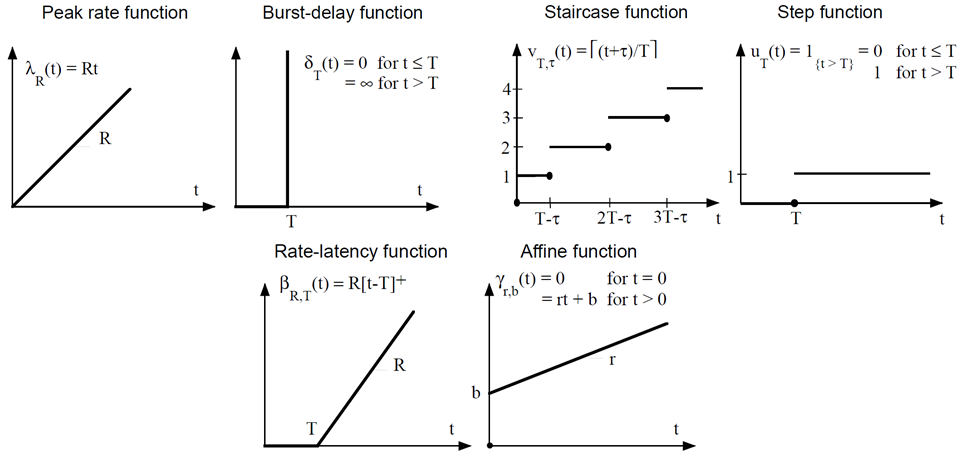
\includegraphics[width=0.95\textwidth]{figs/wsi.png}
  \caption{Example wide sense increasing functions, reprinted from \cite{NCBook}.}
  \label{fig:wsi}
\end{figure}

The main operations of min-plus calculus are the convolution and
deconvolution operations, which act on sub-additive functions.
Convolution is a function of the form:

\begin{equation}
  (f\otimes g)(t)\equiv inf_{\{0\leq s \leq t\}}\{f(t-s)+g(s)\}
\end{equation}

Note that if the functions $f,g$ are concave, this convolution
simplifies into the computation of the minimum:

\begin{equation}
  (f\otimes g)(t)=min(f,g)
\end{equation}

Convolution in min-plus calculus has the properties of 

\begin{enumerate}
\item Closure: $(f\otimes g)(t) \in \mathpzc{F}$,
\item Associativity: $\forall f,g,h \in \mathpzc{F}, (f\otimes
  g)\otimes h = f\otimes(g\otimes h)$,
\item Commutativity: $\forall f,g \in \mathpzc{F}, f\otimes g
  = g\otimes f$, and
\item Distributivity w.r.t. $\wedge$: $\forall f,g,h \in \mathpzc{F},
  f\otimes(g\wedge h) = (f\otimes g)\wedge(f\otimes h)$
\end{enumerate}

Similarly, deconvolution is a function of the form:

\begin{equation} 
  (f\oslash g)(t)\equiv sup_{\{0\leq u\}}\{f(t+u)-g(u)\}
\end{equation}

Note that $\oslash$ is not closed in $\mathpzc{F}$ because $(f\oslash
g)(t)$ is not necessarily $0$ for $t\leq0$.

% MORE INFO ABOUT NC
Network Calculus focuses on abstracting the network traffic and the
computing nodes as \textit{arrival curves} and traffic shaping
\textit{service curves}. The arrival curves and service curves model
the amount of data generated or serviced as functions of time window
size and are bounded by maximum and minimum arrival and service
curves.  By abstracting the network flows and traffic shapers as
arrival curves and service curves, respectively, (min,+) calculus can
be used to compose models of system behavior and calculate performance
characteristics of the integration of the application and the network.

Given an arrival function $R(t)$ for the data flow describing the
number of bits seen on the flow during the time interval $[0,t)$, the
arrival curve $\alpha$ constrains the flow if and only if

\begin{equation}
  \forall s\leq t : R(t) -R(s) \leq \alpha(t-s)
\end{equation}

This relation is shown in Figure~\ref{fig:nc_arrival_curve}.
Intuitively the arrival curve representation transforms the data
production from a function of time, described by $R(t)$, into a
function of time-interval, described by $\alpha(t)$, for which $R\leq
R \otimes \alpha$.

\begin{figure}[htb]
  \centering
  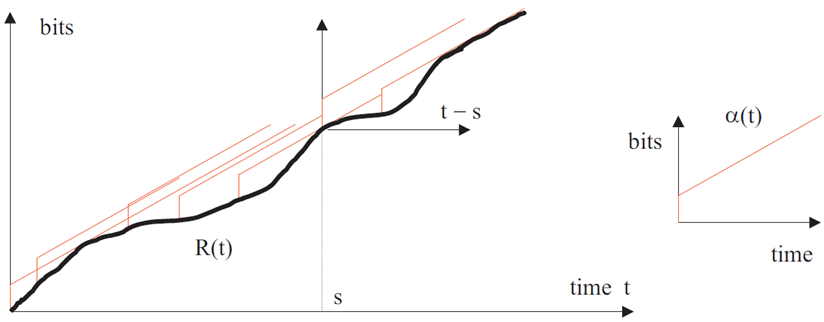
\includegraphics[width=0.95\textwidth]{figs/nc_arrival_curve.png}
  \caption{Illustrative example representing maximum arrival curves
    ($\alpha(t)$) for data flows ($R(t)$), reprinted from
    \cite{NCBook}.}
  \label{fig:nc_arrival_curve}
\end{figure}

Similarly, service curves transform the output data flow $R^*(t)$
into a minimum service curve $\beta$ according to the relation:

\begin{equation}
  R(t)-R^*(t_0)\leq \beta(t-t_0), \forall t\geq 0\ \exists\ t_0\geq
  0,t_0\leq t
\end{equation}

or more compactly $R^*\geq R\otimes\beta$.  This relation is shown in
Figure~\ref{fig:nc_service_curve}.

\begin{figure}[htb]
  \centering
  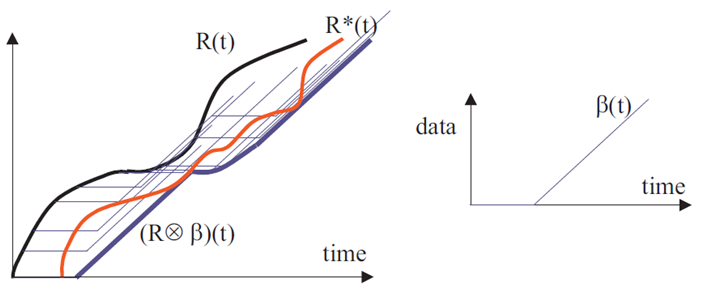
\includegraphics[width=0.95\textwidth]{figs/nc_service_curve.png}
  \caption{Illustrative example representing minimum service curves
    ($\beta(t)$) for output data flows ($R^*(t)$), reprinted from
    \cite{NCBook}.}
  \label{fig:nc_service_curve}
\end{figure}

From the input arrival curve $\alpha$ into a node providing service
curve $\beta$, we can use Network Calculus to compute the output flow
from the node and a few performance bounds governing the buffering
delay and buffer requirements for the node.  The output flow from the
node is constrained by the arrival curve $\alpha^* =
\alpha\oslash\beta$.  Given the arrival curve and service curve for a
node or system, we can compute the backlog and delay bounds, see
Figure~\ref{fig:nc_bounds}; the backlog bound is given by:

\begin{equation}
  R(t)-R^*(t)\leq sup_{\{s\geq 0\}}\{\alpha(s)-\beta(s)\}
\end{equation}

and the delay bound is given by: 

\begin{equation}
  h(\alpha,\beta)=sup_{\{s\geq0\}}[inf\{T:T\geq0\ and\ \alpha(s)\leq\beta(s+T)\}]
\end{equation}

\begin{figure}[htb]
  \centering
  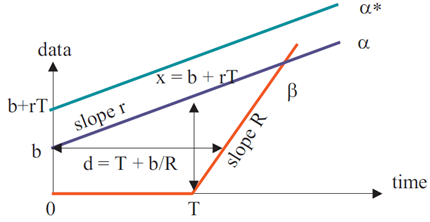
\includegraphics[width=0.75\textwidth]{figs/nc_bounds.png}
  \caption{Illustrative example representing the backlog and delay
    bounds calculated from input arrival curves and node service
    curves, reprinted from \cite{NCBook}.}
  \label{fig:nc_bounds}
\end{figure}

These bounds provide the requisite information needed to make
design-time guarantees about \emph{worst-case} application performance
on the network, given that both the application traffic profile and
the system's network performance are deterministic.

To enable compositional system analysis, Network Calculus allows for
the concatenation of nodes, Figure~\ref{fig:nc_concatenation}, such
that a flow traversing nodes $N_1$ and $N_2$ in sequence, where each
node provides FIFO service curve $\beta_{i=1,2}$, the concatenation of
the two nodes offers a service curve $\beta_1\otimes\beta_2$ to the
flow.  A major advantage of this approach is the ability to "Pay
Bursts Only Once" (PBOO), which is the property that the delay and
buffer bounds are tighter when derived from the concatenation of the
system than they would have been if they were calculated iteratively.
Again, note that this advantage is not applicable to non-FIFO
systems\cite{NCBook}.

\begin{figure}[htb]
  \centering
  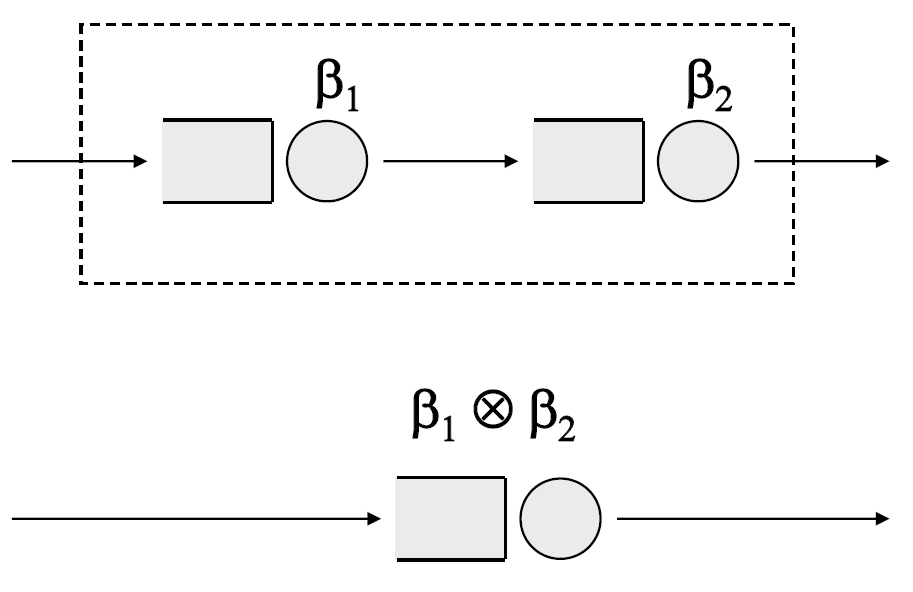
\includegraphics[width=0.75\textwidth]{figs/nc_concatenation.png}
  \caption{Illustrative example representing the concatenation of two
    nodes providing separate services into a single node providing an
    aggregate service, reprinted from \cite{NCBook}}
  \label{fig:nc_concatenation}
\end{figure}

However, the performance bounds calculated by Network Calculus are
still worst-case performance based.  For instance, there is a temporal
disconnect between the arrival/service curves and the actual
performance of the application or the system.  This disconnect leads
to analysis results that may still over-approximate the required
buffer size or application delay on the network.  The cause of this
over-approximation comes from the use of \emph{time windows}.  Because
Network Calculus is focused on maximum data produced and minimum data
serviced as functions of time window size, the time-varying nature of
the data production or service is lost.  Despite an application
producing a Bulk Data Transfer (BDT) during a period of high network
resource availability, Network Calculus compares that BDT to all
windows of time throughout the service time of the system.  As such,
an expected drop in service during a different period of time will
inadvertently negatively affect the application's predicted
performance as analyzed by Network Calculus.

\subsubsection{Real-Time Calculus}
\label{subsec:rtc}
Real-Time Calculus\cite{Thiele00real-timecalculus} builds from Network
Calculus, Max-Plus Linear System Theory, and real-time scheduling to
analyze systems which provide computational or communications
services.  Unlike Network Calculus, Real-Time Calculus (RTC) is
designed to analyze the impact of real-time scheduling and priority
assignment in task service systems.  The use of (max,+)-calculus in
RTC allows specification and analysis not of only the arrival and
service curves described above for Network Calculus, but of upper and
lower arrival curves ($\alpha^u(\Delta)$ and $\alpha^l(\Delta)$) and
upper and lower service curves ($\beta^u(\Delta)$ and
$\beta^l(\Delta)$).  These curves represent the minimum and maximum
computation requested and computation serviced, respectively.  An
overview of RTC is given in Figure~\ref{fig:rtc_overview}.

\begin{figure}[htb]
  \centering
  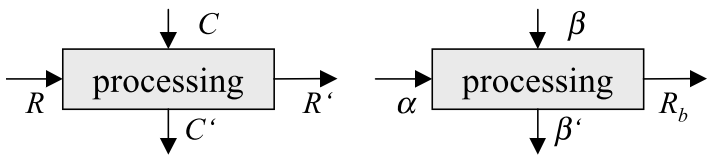
\includegraphics[width=0.75\textwidth]{figs/rtc_overview.png}
  \caption{Overview of Real-Time Calculus' request, computation, and
    capacity models.  $R(t)$ is the request function that represents
    the amount of computation that has been requested up to time $t$,
    with associated minimum request curve, $\alpha$.  $R'(t)$ is the
    total amount of computation delivered up to time $t$, with
    associated delivered computation bound $R_b(t)$.  $C$ and $C'$ are
    the capacity function and remaining capacity functions which
    describe the total processing capacity under full load and the
    remaining processing capacity, respectively.  $C$ and $C'$ are
    bounded by the delivery curve $\beta$ and the remaining delivery
    curve $\beta'$, reprinted from \cite{Thiele00real-timecalculus}.}
  \label{fig:rtc_overview}
\end{figure}

\begin{figure}[htb]
  \centering
  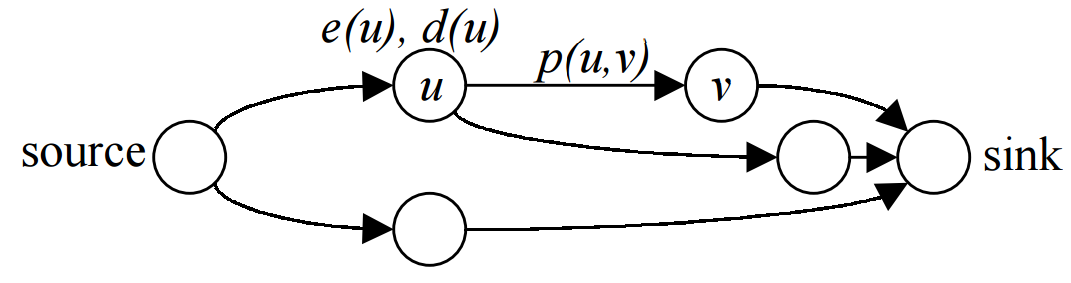
\includegraphics[width=0.75\textwidth]{figs/task_graph.png}
  \caption{An example task graph for Real-Time Calculus, with
    conditional branches; reprinted from
    \cite{Thiele00real-timecalculus}}
  \label{fig:task_graph}
\end{figure}

RTC allows for the analysis of task scheduling systems by computing
the request curve for a task model which is represented as a directed
acyclic graph (DAG), the task graph $G(T)$.  An example task graph is
shown in Figure~\ref{fig:task_graph}.  The graph's vertices represent
subtasks and each have their own associated required computation time
$e(u)$, and relative deadline $d(u)$ specifying that the task must be
completed $d(u)$ units of time after its triggering.  Two vertices in
$G(T)$ may be connected by a directed edge $(u,v)$ which has an
associated parameter $p(u,v)$ which specifies the minimum time that
must elapse after the triggering of $u$ before $v$ can be triggered.
RTC develops from this specification the minimum computation request
curve $\alpha_r$ and the maximum computation demand curve $\alpha_d$.
Finally, the schedulability of a task $T_i$ is determined by the
relation:

\begin{equation}
  \beta'(\Delta)\geq\alpha^i_d(\Delta)\ \ \ \forall\Delta
\end{equation}

which, if satisfied, guarantees that task $T_i$ will meet all of its
deadlines for a static priority scheduler where tasks are ordered with
decreasing priority.  Note that the remaining delivery curve
$\beta'(\Delta)$ is the capacity offered to task $T_i$ after all tasks
$T_{1\leq j<i}$ have been processed. Similarly to Network Calculus,
RTC provides analytical techniques for the computation of performance
metrics such as computation backlog bounds:

\begin{equation}
  \text{backlog}\leq sup_{\{t\geq 0\}}\{\alpha^u(t)-\beta^l(t)\}
\end{equation}

which is equivalent to the network backlog bound derived in Network
Calculus.

\cite{RTCcomparison2011} compares different analytical methods for
network performance analysis, namely Real-Time Calculus (RTC),
probabilistic queuing models, parallel computation models, and
protocol offload models.  The authors explain the current state of
system evaluation, which is based predominantly on quantitative
evaluation through simulation, but make the point that such simulation
techniques should be used sparingly since \textit{only a finite state
of initial states, environment behaviors, and execution traces can
be considered by system simulators}.  The system which the authors
model for their comparison is the case of Network Interface Cards
(NICs) connected to a Local Area Network (LAN), for which they derive
analytical bounds on the buffer requirements as they are affected by
the input/output (I/O) subsystems, the network traffic, the NIC
itself, and the memory controllers.  They point out that most
researchers are still using Queuing Theory, in stochastic scenarios
where the network traffic is modeled as random distributions of data.
Because RTC allows more precise descriptions of application traffic,
it can be more beneficial for providing analysis of buffer
requirements and delay experienced in the system.  RTC's ability to
allow such specifications comes from its roots in Network Calculus and
Max-Plus Linear System theory.

\subsubsection{Stochastic Network Calculus}
% STOCHASTIC NETWORK CALCULUS
These deterministic constraints can be relaxed so that the
deterministic arrival and service curves are instead replaced by
stochastic processes, causing the bounds on the performance to be
probabilistic as well\cite{Burchard06amin-plus}.  As described
previously, these probabilistic performance bounds may not be precise
enough to provide the types of guarantees required by certain classes
of mission- or safety-critical systems.

\cite{SNC80211backlogdelay2011} provides a good description, system
model, and analysis for stochastic Network Calculus applied to
wireless networks.  In their work, they show the ability of network
calculus to remove the need to make as many assumptions about the
arrival or service processes (\emph{e.g.} exponential service
distribution) to allow general arrival and service processes.  They
apply stochastic network calculus to analyze backlog and delay bounds
in 802.11 based multi-access systems.  They formally derive bounds for
the backlog and delay in the network and then compare these analytical
results to bounds generated from network simulation using ns-2.  From
this comparison, they conclude that the derived bounds are too loose
and in fact get looser the closer the system gets to saturation.  They
further conclude that this looseness is a direct result of stochastic
network calculus itself, and claim that it requires further
improvements.  It is important to remember what was stated previously
by \cite{simulator_comparison_2003}: the simulation does not
accurately model the dynamic behavior of real traffic, so the results
from \cite{SNC80211backlogdelay2011} may too be inaccurate.

Because Network Calculus deals with either deterministic worst-case
application performance on a static network or stochastic application
performance on a dynamic network, system designers and application
designers under-utilize the network resources of systems which require
strict design-time guarantees about application performance.

\subsubsection{Extensions to Network Calculus}
% OTHER ADAPTATIONS AND ADDITIONS TO NC
When analyzing any complex system, the fidelity of the analysis
results with respect to the actual system relies heavily on the level
of detail of the models of the system's components and
subsystems. \cite{Heidemann2001} covered the effects that different
levels of detail have on analysis complexity and accuracy.
Importantly, they point out the requirement to not only be correct,
but also be applicable, \emph{i.e.} analysis results should be both
accurate with respect to the system being modeled, but should also be
relevant for the analysis and development of real systems.
Additionally, they point out that not all systems require highly
detailed modeling for the analysis results to be correct, since some
systems and applications are insensitive to lower level details.

There are many efforts to make analytical techniques more
representative of actual systems in order to increase the fidelity of
the analysis results with respect to the run-time system.  The
researchers in \cite{NCnetworkCoding} recognize the need to analyze
not only the overall throughput of a network, but also the end-to-end
delay experienced by information flows in the network.  Furthermore,
they derive an analytical model of Wireless Network
Coding\cite{networkcodingCOPE}, a technique for combining packets
together for improving network throughput in wireless networks using
broadcast techniques.  They show that by developing a model of the way
the MAC layer works in the network and how the information flows are
combined and disseminated, they can get tighter performance bounds and
even derive methods for increasing performance in the network by
altering the scheduling parameters of the packet flows.  Analyzing
multiple performance parameters, in this case the network throughput
and end-to-end delay, is a key element for analyzing and providing
quality of service (QoS) to applications.

The authors in \cite{NCpacketcurve2012} also incorporate more precise
models of the network to derive tighter performance bounds using
Network Calculus.  They show that by modeling the packetization that
occurs in the network using a \textit{packet operator} to transform
arrival flows into packet flows, they can analytically derive tighter
service curves than would be found from traditional Network Calculus.
Clearly, there exists a desire from application developers and system
integrators to derive both accurate and precise design-time
performance parameters for the system and its applications.

Similarly, in \cite{NCspacewire}, the authors describe how to
accurately model the SpaceWire network standard which has been
developed for satellites in the European Space Agency (ESA).  Their
network must be shared by both real-time (critical) and non real-time
(non-critical) traffic, but the system developers require design-time
guarantees about the temporal characteristics of all
critical/real-time messages on the network.  Their work focuses on
accurately representing the SpaceWire network, its (static) routing
protocol, and the service profiles of its routers including the
aspects of their flow control algorithms.  Building on previous work,
they explain the need, for resource-constrained real-time systems, to
accurately model the network traffic in order to derive a model of the
network which is not too pessimistic.  They derive accurate Network
Calculus/Real-Time Calculus (RTC) based models of the wormhole
switches present in the network and show the fidelity of their
analytical tools compared with the industrial simulation tools
developed for SpaceWire networks.  Using a Network Calculus-based
model, they are able to achieve analytical results that are the same
order of magnitude as the simulation results for the critical traffic
delay characteristics, but are less precise for the non-critical
traffic in the network.  One important point they make that extends to
all types of systems when comparing analysis and simulation techniques
is this: \textit{worst-case delays can be extremely rare events which
are hard to observe or recreate in simulations, but can be derived
from analytical results.}\cite{NCspacewire}

Another approach to increasing the fidelity of the analysis is to
model the Time Division Multiple Access (TDMA) medium channel access
protocol using Network Calculus to derive performance
metrics\cite{Schmitt2007}.  TDMA service curves are modeled such that
the medium's transmit capacity is available to the node only during
the node's designated slot.  During all other slots of the TDMA
period, the medium's capacity is unavailable to the node and therefore
the transmit capability of the node is zero.  As such, simple TDMA
service curves can be described using simply a slot length, a slot
bandwidth, and a TDMA period.

\cite{TDMA_Khan_98} analyzes the performance of TDMA with respect to
the queue size for different probabilistic traffic models, and shows
how the G/D/1 model with application-based probability distributions
can be used to generate closed-form solutions for analyzing arbitrary
traffic on a TDMA network.

Another aspect of system design which has been gaining momentum is the
development of self-adaptive systems which provide "self-*" properties
such as self-management.  These types of systems are typically not
used in CPS control applications or other systems which require
real-time guarantees about timing or resource properties of the
system.  The main reason for their absence from these types of systems
and applications is the lack of available, accurate modeling and
analysis techniques which properly capture the behavior of the
applications in a way that allows the derivation of performance
guarantees.  The authors in \cite{NCadaptivesystems} describe both the
need for this type of analysis for these systems and describe the
overview of how the analysis would work, based on concepts from
Network Calculus.  Their main point is that currently such types of
analysis tools do not exist for these systems, which makes developing
the systems difficult with respect to these types of design
parameters.  They propose developing a formalized standardization for
the self-adaptive behavior, which they present as a state-space with
available control actions based on the sensor data in the system.

%%%%%%%%%%%%%%%%%%%%%%%%%%%%%%%%%%%%%%%%%%%%%%%%%%%%%%%%%%%%%%%%%%%%%%%%%%%%%%%%%%%
%%%%%%%%%%%%%%%%%%%%%%%%%%%%%%%%%%%%%%%%%%%%%%%%%%%%%%%%%%%%%%%%%%%%%%%%%%%%%%%%%%%
%%%%%%%%%%%%%%%%%%%%%%%%%%%%%%%%%%%%%%%%%%%%%%%%%%%%%%%%%%%%%%%%%%%%%%%%%%%%%%%%%%%
%%%%%%%%%%%%%%%%%%%%%%%%%%%%%%%%%%%%%%%%%%%%%%%%%%%%%%%%%%%%%%%%%%%%%%%%%%%%%%%%%%%
%%%%%%%%%%%%%%%%%%%%%%%%%%%%%%%%%%%%%%%%%%%%%%%%%%%%%%%%%%%%%%%%%%%%%%%%%%%%%%%%%%%
\section{Part 2: Run-Time Network Monitoring and Management}
\label{sec:related_part2}

In addition to design-time modeling and analysis, CPS system designers
and integrators must ensure system stability during run-time by
enforcing resource limitations on the applications to ensure no faulty
or malicious code starves the system or other applications of network
resources.  Such enforcement is the management of the network resource
for the system.  Many different approaches exist to handle this type
of management, generally falling into one of two categories: (1)
static management or (2) dynamic management.  Static management of
system resources is based around enforcement of fixed resource
allocations which were decided at design-time or deployment time.
Such management generally is associated with high-criticality systems
which must be guaranteed.  Dynamic management of resources entails
updating the resource allotments of each application based on
currently available system resources and application load, and
generally is in the class of adaptive management or adaptive systems
(also called autonomic systems).  In this work, we will address only
static management of resources.

Static management of network resources generally, but not necessarily,
means applications are given a fixed quantity of resources for the
lifetime of the system.  The part of the system which enforces these
resource allotments however, may vary depending on the design of the
system.  The enforcement may happen in the network layer, in the
operating system kernel, or in some cases in the middleware
facilitating the network communications for the applications.  We deem
any enforcement happening in the kernel or in a lower layer to be
\textit{infrastructural management} (since all applications on the
system must use this infrastructure and are therefore managed by it).
We deem any resource management happening between the kernel and the
application as \textit{middleware management}, since different
applications deployed on the system may use different middleware
stacks and therefore may be managed differently.


\subsection{Infrastructural Approaches for Network Management}
\label{subsec:related_part2_infrastructural}

Two of the main infrastructural methods for managing system network
service are DiffServ\cite{rfc2474}\cite{QT_Giambene2005} and
Intserv\cite{rfc1633}.  DiffServ, for Differentiated Services, is
designed for the provisioning of network resources to provide Quality
of Service (QoS) to applications on the network but is unable to
provide strict real-time guarantees about packet loss, delay, and
bandwidth availability.  Instead, DiffServ was designed to scale well
for large systems while still providing probabilistic guarantees.
IntServ, for Integrated Services, was designed to provide strict
real-time guarantees about the QoS experienced by a flow on the
network.  Unlike DiffServ, which does not maintain any state
information in the routers along network flow paths, IntServ uses a
resource reservation protocol (RSVP)\cite{rfc2205} with explicit setup
of flows for deterministically allocating bandwidth and buffer space
for a flow in each router along the flow's path.  While such an
explicit out-of-band QoS reservation protocol enables similarly
explicit resource availability and performance guarantees, the
trade-off comes in the ability of the system to scale to many nodes
and many flows.  DiffServ's scalability comes from both the lack of
explicitly maintaining per-flow state in the routers, by assigning
traffic to a set of predefined classes, as well as using QoS
assignment mechanisms which are built into the flow's messages,
e.g. the DiffServ Code Point (DSCP) built into the Type of Service
(ToS) byte in IPv4 headers and the Traffic Class byte of IPv6 headers.

Both IntServ and DiffServ were originally designed for wired networks,
but \cite{diffServ_intServ_Mahadevan1999} has worked on the required
modifications to make them suitable for wireless networks, which have
network connectivity and link characteristics which have more variance
as a function of time.  The combination of low bandwidth, high loss,
and node mobility require extensions to the QoS parameters and control
options available to the application provided by the QoS
infrastructures.  One such proposed extension is the concept of loss
profiles, which govern whether an application prefers dropping data in
a bursty manner (as might be preferred by audio applications) versus a
distributed manner (as might be preferred by video applications).
Similarly, since link bandwidth is typically much lower than in wired
networks, IntServ/RSVP's refresh messages (used to determine network
changes) should be sent with a lower frequency to provide as much
network bandwidth as possible to application traffic.  In the same
way, DiffServ requires modifications to support signaling information
about link state and node location to overcome DiffServ's static
provisioning scheme in the adaptation from wired to wireless networks.

A system's network infrastructure may provide multiple different QoS
provisioning implementations, such as both DiffServ and IntServ.  In
this case, the applications can select which QoS provisioning to use.
Similarly, large networks may be grouped into subnets which each
internally use different QoS provisioning schemes.  The boundaries
between these subnets requires QoS mapping for flows which cross these
boundaries.  Such mapping between QoS implementations and
configurations is complex and makes providing guarantees about QoS for
large complex networks challenging.

Because both IntServ and DiffServ were designed for providing QoS to
generic traffic for large networks including the internet, they were
not designed to be able to provide performance guarantees to
application developers.  As such, their design and implementation
function more coherently in a system which has unknown applications
and application load.  However, the classes of systems we focus on
require more precise guarantees about performance and have the benefit
of more precise design-time knowledge of applications and application
load on the system.

%TALK ABOUT QoS MODEL FOR MANET (3)
Flexible QoS Model for Mobile Ad-hoc Networks (MANETs),
FQMM\cite{Xiao2000}, attempts to address the issue of run-time QoS
management and adaptation to changing environmental conditions
affecting the network.  Recognizing that both environmental and
application behavior need to be taken into account for QoS management,
they argue that two methods for providing QoS in the internet, IntServ
and DiffServ, are not sufficient for dynamic mobile networks.  While
IntServ's scalability problem will not affect dynamic mobile networks
in the near future, they argue that the connection maintenance
required by the Resource ReSerVation Protocol (RSVP) renders IntServ
impractical.  DiffServ, on the other hand, might be able to provide
long-term QoS to applications under the varying network conditions,
but is not feasibly able to provide the kind of short-term QoS
required by real-time applications.  Furthermore, DiffServ does not
handle node mobility and external disturbances from the environment
well as it was originally designed for relatively fixed
(topologically) networks.

To combat the issues in both IntServ and DiffServ, FQMM is designed to
handle QoS for MANETs.  FQMM focuses on allowing for fine-grained
provisioning of node resources and allowing node mobility through
dynamically reassigning the roles of each of the nodes in the network.
The provisioning of the resources for flows in the network borrows
ideas from both IntServ and DiffServ by combining the per-flow
granularity of IntServ for high-priority flows while lower-priority
flows are provisioned on a class basis as in DiffServ.  This
differentiation between traffic classes and priority flows better
utilizes the system resources to achieve the necessary performance for
high priority flows which may need real-time performance.  To provide
traffic shaping they constrain the bandwidth of flows to traffic
profiles, which govern the latency and bandwidth available to the
flow. To combat the time-varying nature of the network, they instead
define these traffic profiles as a percentage of the available network
bandwidth.  This type of percentage-based flow constraint limits the
adaptability of the network traffic however, as certain
higher-priority real-time flows may have a minimum amount of bandwidth
required that cannot be met with a percentile constraint on effective
link bandwidth.  FQMM also addresses routing control to provide better
run-time QoS to applications on the system.

\subsection{Middleware Based Approaches for Network Management}
\label{subsec:related_part2_middleware}

For system and application level adaptation to changing system
resources, two main approaches, namely fixed reservation of flows and
run-time adaptation, provide benefits for performance or resilience.
These two approaches cannot be used alone however, as fixed
reservation of flows based on design-time network analysis causes low
resource utilization and run-time adaptation is generally not prepared
for excessive congestion or other disturbances.  GARA
\cite{Foster2000} combines these two paradigms to provide more
graceful degradation and higher resource utilization at the system and
application level.  GARA uses priority based flow reservation which
can be altered at run-time by both the application and by third
parties on behalf of the application.  This type of reservation scheme
allows applications to monitor and react to changes in network
capacity, while still attempting to ensure that high-priority flows
can traverse the network.  Furthermore, this type of reservation
scheme is more amenable to dynamic flows which may only be active
during a portion of time that the system is active.  Statically
defined slots reserved at design-time cause wasted resources by these
applications whose flow is reserved but not used the entire time.

%DDS QoS options; need other examples

Finally, there do exist different protocols and communications
paradigms which support run-time control of application network
traffic, such as the Quality of Service (QoS) control mechanisms
present in many implementations of OMG's Data Distribution Service
(DDS) standard\cite{OMG-DDS:07}\cite{OpenDDS:07}.  However, often the
mechanisms available for controlling the QoS parameters of a given
data stream are complex, interacting mechanisms which may be difficult
for the application developer to understand and therefore are also not
amenable to modeling and analysis at design
time\cite{Hoffert:2010:AED:1862821.1862825}.  Furthermore, the
developers may not be provided with or have control over lower level
implementation details such as the selected transport layer protocol,
which may affect the available QoS or may not be fully supported by
the infrastructure.  Additionally, many of the available interaction
paradigms either do not support design time QoS analysis with run-time
monitoring and control or the supported QoS analysis and control
interfaces are only informally specified.


\chapter{Design-Time Network Performance Analysis of Distributed CPS Applications}
\label{ch:designTime}

In this chapter, we describe research results related to the
challenge of accurately predicting network QoS for systems which may
require strict guarantees about performance and resource utilization.

Many CPS applications require networking of some form in order for the
system to function nominally.  This networking often performs a key
role in the system, such as facilitating the communication and control
of distributed sensors and control systems.  Traditionally, these
networks of CPS have been both isolated from external influences and
predefined at system design-time.  This isolation and
pre-determination creates a static network with respect to both the
topology of the network and the capacity of each network link.  More
recently however, CPS have become less isolated and more dynamic by
utilizing heterogeneous and wireless networks and incorporating
mobility.  Such systems include wireless sensor networks (WSN), mobile
ad-hoc networks (MANETs), and distributed real-time embedded systems
(DRES).  These types of systems are being developed to provide remote
sensing and control capabilities, smart grid and smart city
infrastructure, and smart vehicle communications networks, to name a
few.

Analyzing application and system network Quality of Service (QoS)
requires either design-time models and analysis techniques or
experimental measurements from an application and system testbed.  For
high- or mixed-criticality software and systems, typically
experimental measurements are used but often these can be incomplete
or quite costly to generate.  Instead, a design-time modeling paradigm
for networked applications and systems can provide developers and
system integrators the information to accurately predict the system
and application network QoS.

\begin{figure}[ht!]
  \centering
  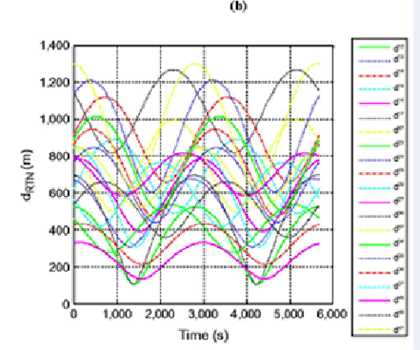
\includegraphics[width=0.85\textwidth]{figs/satellite_network.png}
  \caption{Distance as a function of time (pairwise) between
    satellites in a cluster orbiting Earth.  The network capacity
    varies for each network link between two satellites inversely
    proportional to the distance between them.}
  \label{fig:satellite_network}
\end{figure}

Some wireless mobile CPS networks, such as the network between a
cluster of satellites orbiting Earth, vary periodically with respect
to time, \emph{e.g.} according to the cluster's orbital period.  An
example of such periodic variation in satellite network capacity is
shown in Figure~\ref{fig:satellite_network}.  For such networks, the
physical dynamics of the nodes in the cluster are well understood and
predictable, therefore the network dynamics can be fairly predictable
as well.  For such predictable or periodic dynamic networks, the use
of worst-case network performance for analysis and constraint
verification wastes the network resources over much of the lifecycle
of the system. Integrating the physical dynamics of the network into
the modeling and analysis tools improves the performance of the
systems without degrading its reliability.

%%%%%%%%%%%%%%%%%%%%%%%%%%%%%%%%%%%%%%%%%%%%%%%%%%%%%%%%%%%%%%%%%%%%%%%%%%%%%%%%%%%
%%%%%%%%%%%%%%%%%%%%%%%%%%%%%%%%%%%%%%%%%%%%%%%%%%%%%%%%%%%%%%%%%%%%%%%%%%%%%%%%%%%
%%%%%%%%%%%%%%%%%%%%%%%%%%%%%%%%%%%%%%%%%%%%%%%%%%%%%%%%%%%%%%%%%%%%%%%%%%%%%%%%%%%
%%%%%%%%%%%%%%%%%%%%%%%%%%%%%%%%%%%%%%%%%%%%%%%%%%%%%%%%%%%%%%%%%%%%%%%%%%%%%%%%%%%
%%%%%%%%%%%%%%%%%%%%%%%%%%%%%%%%%%%%%%%%%%%%%%%%%%%%%%%%%%%%%%%%%%%%%%%%%%%%%%%%%%%
\section{Precise Modeling of Application Network Traffic and System Network Resources for Performance Prediction}
\label{sec:framework} 

To precisely predict network performance for applications distributed
in a mobile CPS, we need precise models of both the application
network resource requirements and the system's network resource
capacity.  These predictions, if precise and reliable enough, can
serve as guarantees for application developers and system integrators
about the network QoS that the system will provide and the network
resources the application will receive.

\subsection{Problem}
Current design tools do not incorporate the physical dynamics of the
network for analysis of network constraints on the applications. For
systems with known models of system dynamics, the system's dynamics
should be incorporated into the modeling tool and should integrate
with the other models of the system, e.g. the system's network models.
Because of the diversity of CPS, IoT systems, and other networked
embedded systems in general, modeling and analysis tools targeted
towards these systems must support a wide range of configurations,
architectures, standards, and interfaces.  The same compatibility is
required in network modeling and analysis frameworks.  Because many of
these systems may support different types of network communications
hardware, often using multiple types of network interface hardware
within the same system, the models of the network must be able to
express network resources in a way that can capture these differences.
Because of this diversity and the modeling semantics of the commonly
used paradigms (e.g. Real-Time Calculus), developing very precise
predictions is difficult, since the models are not very precise with
respect to the actual behavior of the applications on the system.

\subsection{Mathematical Formalism}
\label{subsec:math_formalism}

To model the network capability of the system and the application
traffic patterns, we have developed a network modeling paradigm
similar to Network Calculus' traffic arrival curves and traffic shaper
service curves.  This paradigm is called \fulltool/ (\shorttool/). 

Similarly to Network Calculus' arrival curves and service curves, our
network profiles model how the system's network performance or
application traffic generation changes with respect to time.  Whereas
Network Calculus' modeling transforms application data profiles and
network service profiles into max/min curves for data
received/serviced vs. length of time-window, our models take a simpler
approach which models exactly the data generated by the application
and the data which could be sent through the network, allowing our
performance metrics to be more precise.  Specifically, the bandwidth
that the network provides on a given communication link is specified
as a periodic time series of scalar bandwidth values. Here, bandwidth
is defined as data rate, i.e. bits per second, over some averaging
interval.  This bandwidth profile can then be time-integrated to
determine the maximum amount of data throughput the network link could
provide over a given time.  The bandwidth profile for the application
traffic similarly can be time-integrated to determine the amount of
data that the application attempts to send on the network link as a
function of time.

Having time-integrated the bandwidth profiles to obtain data vs. time
profiles that the application requires and that the system provides,
we can use a special type of convolution ($\otimes$),
\emph{(min,+)-calculus convolution}, on these two profiles to obtain
the transmitted link data profile as a function of discrete time. The
convolution we define on these profiles borrows concepts from the
min-plus calculus used in Network Calculus, but does not use a
sliding-window and instead takes the transformed minimum of the
profiles. For a given application data generation profile, $r[t]$, and
a given system link capacity profile $p[t]$, where $t\in\mathbb{N}$,
the link transmitted data profile $l[t]$ is given by the convolution
Equation~\ref{eq:convolution}. The difference $(p[t-1] - l[t-1])$
represents the difference between the amount of data that has been
transmitted on the link $(l[t-1])$ and the data that the link could
have transmitted at full utilization $(p[t-1])$. As demonstrated by
the convolution equation, $\forall t : l[t] \le r[t]$, which is the
relation that, without lower-layer reliable transport, the link cannot
transmit more application data for the application than the
application requests.  Note that there will be packetization and
communication header overhead which will be transmitted with
application data.  The overhead can be determined at design time and
can therefore be accounted for in the application profile.

\begin{equation}
	\label{eq:convolution}
	\begin{split}
		y=l[t] &= (r \otimes p)[t] \\ &= min( r[t] , p[t] -
                (p[t-1] - l[t-1]) )
	\end{split}
\end{equation}
\vspace{-0.5in}
\begin{align}
	\label{eq:buffer}
	&\text{buffer}= sup\{r[t] - l[t] : t \in \mathbb{N}\}\\
	\label{eq:delay}
	&\text{delay} = sup\{l^{-1}[y]-r^{-1}[y] : y \in \mathbb{N}\}
\end{align}

\begin{figure}[h!]
	\centering
        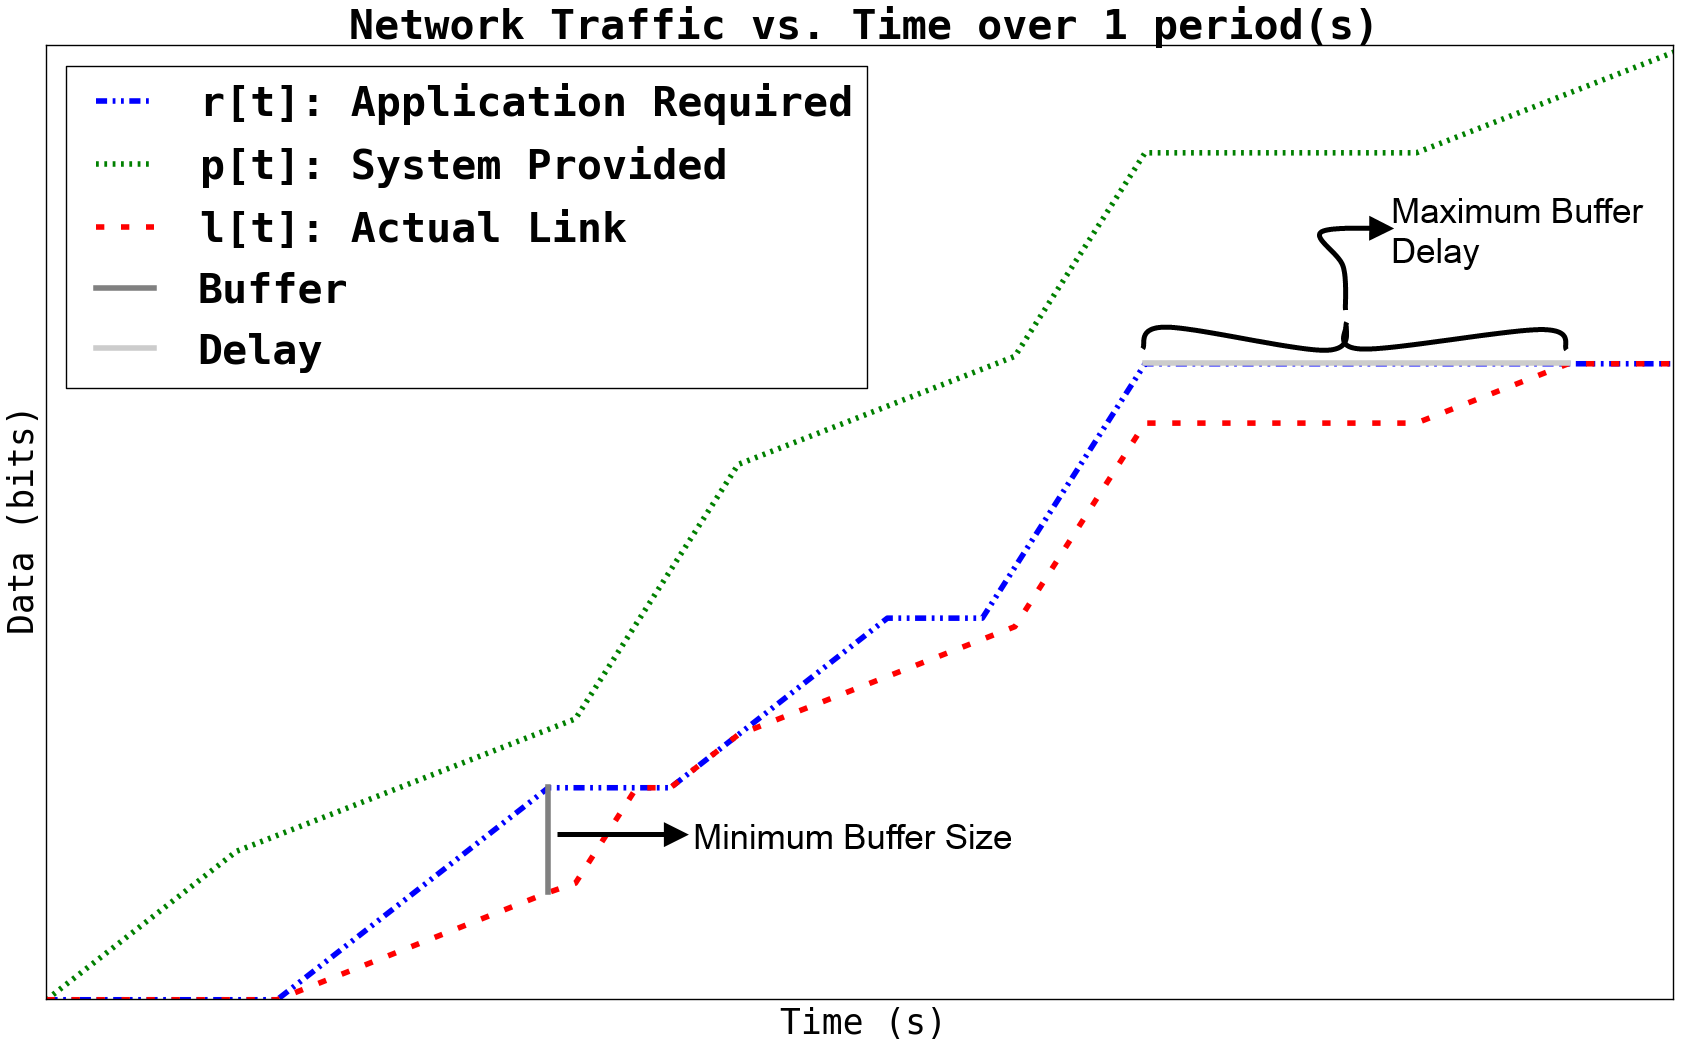
\includegraphics[width=0.85\textwidth]{figs/convolution6.png}
	\caption{Representative example demonstrating convolution of
          the data vs. time profiles that the application requires and
          that the system provides.  The resultant data vs. time
          profile describes the data that the system actually
          output onto the link.}
	\label{fig:convolution}
\end{figure}

Equation~\ref{eq:buffer} and Equation~\ref{eq:delay} calculate, using
$l[t]$, $r[t]$, and the inverse function $l^{-1}[y]$, the minimum
buffer size required for the application and the maximum buffering
delay experienced by application data, respectively.
Figure~\ref{fig:convolution} depicts the convolution operation and
shows a schematic representation of the maximum buffer delay and the
minimum buffer size.  As can be seen in the figure, the maximum
horizontal distance between the required profile and the link profile
is equal to the maximum buffer delay, while the maximum vertical
distance is equal to the minimum buffer size required for loss-less
transmission of data on the link.

We developed the \shorttool/ paradigm to precisely
model system network resources as they vary with respect to time.
Similarly, the application network resource requirements can be
modeled very precisely as functions of time.  These models can be more
precise than the models developed for Network Calculus since they are
explicitly functions of time, instead of functions of time-windows.
Taking the example from earlier, a bulk data transfer (BDT) initiated
from the satellite cluster to a ground station is scheduled for when
the satellite cluster is within range of the ground station and
therefore has a good downlink to the ground.  With our paradigm, this
coupling between the network traffic flow and the network resource
availability can be captured explicitly in the model.  Under the
Network Calculus modeling semantics however, such a BDT would
negatively affect the predicted required network buffer size and
network buffering latency since that BDT data transmission window
(i.e. the window of time it sends the data on the link) would be
compared against the minimum service provided by the network to the
ground station (which would be zero during the parts of the orbit when
the ground stations are not within range of the cluster).  Such a
comparison drastically increases the predicted buffer space required
and predicted buffering latency incurred by the BDT data.

This network modeling and analysis technique we developed has been
reported in \cite{ISIS_F6_CYPHY:14}, which describes the network
resource models, their composition, and the calculation of performance
metrics such as buffer requirements and buffering delay.

\subsection{Accuracy and Precision}
\label{subsec:precision}

When developing a new analysis technique to predict application
network performance, verification that the results of the analysis are
accurate is paramount.  Experimental results are required not only to
judge whether or not the theory is sound, but also to allow
application developers and system integrators to judge the
applicability of the analysis to their systems and applications.  If
the error in the predicted performance metrics is too high, the
analysis results will cease to be useful.

We developed a network emulation testbed which applies the system's
time-varying network profile to all network traffic in the system, and
has been reported in \cite{ISIS_F6_CYPHY:14}.  On this testbed we ran
application network traffic generation code which produces network
traffic according to the supplied application profile.  This traffic
generation code measured the delay, throughput, and buffer
requirements of the traffic that was generated.  By collecting these
measurements over the course of multiple tests, we measured the
differences between the predicted and measured buffer size and delay.
The accuracy of our prediction was reported in
\cite{ISIS_F6_CYPHY:14} and is shown in \ref{table:results}.

\begin{table}[htbp]
\caption{Network utilization calculations and measured results using UDP over IPv6.}
\begin{tabular}{| c | c | c |}
\hline
 & Predicted & Measured ($\mu,\sigma$) \\\hline
Buffer Delay (s) & 0.0625 & (0.06003 , 0.00029) \\\hline
Time of Delay (s) & 3.0 & (2.90547 , 0.00025) \\\hline
Buffer Size (bytes) & 8000 & (7722.59 , 36.94) \\\hline
\end{tabular}
\label{table:results}
\end{table}

\subsection{Assumptions Involved}
\label{subsec:assumptions}

As with any type of system modeling and analysis paradigm, it is
important to remain aware of the types of systems the
modeling/analysis is applicable to, the requirements imposed on the
system by the model, and any edge cases or scenarios where the
analysis or modeling paradigm breaks down.

The major assumption that we make with this type of system modeling
and analysis is that we \emph{can} know at design time what the system
network capacity and the application data production will be as a
(possibly periodic) function of time.  Of course, this assumption is
unrealistic for heavily data-dependent systems, but by performing some
code analysis and/or doing some controlled experiments, models of the
applications' behavior can be developed that can be analyzed.

Another key assumption and thus requirement of our modeling and
analysis framework is a system-wide synchronized clock which all nodes
use.  By this we mean that if two nodes produce data for a third node
at time $t=3$ seconds, they will produce their data onto their
respective network links at exactly the same time.  This is required
for the composition of profiles as they traverse the network and are
routed through nodes.  This assumption restricts the types of systems
for which our analysis can be most useful, but is not a critical
hindrance, as many such critical systems, e.g. satellite
constellations or UAVs have GPS synchronized clocks, which provide
such a foundation.

Another restriction with our modeling paradigm is that data-dependent
flows cannot be accurately represented, since we have no way of
modeling data-dependence.  A related assumption is processing power
and the ability of the software to adhere to the profiles: we assume
the applications are able to accurately and precisely follow their
data production profiles, regardless of the number of other components
on their hardware node.  Similarly, we assume that under all
circumstances, the service profile of a hardware node will be adhered
to.

Finally, we have currently not incorporated the ways different
reactive protocols would affect system network analysis.  A common
example of such a reactive protocol is TCP and its congestion
avoidance algorithm.  Because such algorithms rely on return-path
information through the use of handshaking/acknowledgements they
provide greater difficulty in modeling and analysis.  As such, we have
focused primarly on one-way transmission and reception style
interactions for our modeling and analysis.  Such types of
interactions are found for instance in UDP transmissions.  

\subsection{Factors Impacting Analysis}
\label{subsec:impacts}

It is important when developing modeling and analysis techniques to
analyze how the analysis time and results are affected by changes in
the model.  This is especially true when trying to determine how
applicable new techniques are to large scale systems.  Models are
provided by the application and system developers and are described in
the form of bandwdith (bps) vs time that the application requires or
the system provides.  These profiles are a time series that maps a
given time to a given bandwdith.  Between two successive intervals,
the bandwidth is held constant.  Clearly, to represent changing
bandwidth over time, the developer must use sufficiently short enough
time intervals to allow step-wise approximation of the curve.
However, as with any system, there is a tradeoff between precision of
the model and the analysis time and results.

Because the fundamental mathematics are linear for our convolution,
our convolution scales with $O(n)$, where $n$ is the total
number of intervals in all of the profiles analyzed.  It is worth
noting that this complexity is not the same as the $O(n^2)$ or
$O(n*log(n))$ complexity that traditional convolution has.  This
decrease in complexity is due to our convolution only requiring a
single operation (comparison operation for the minimum) for each value
of $t$.  As such, each element in both of the profiles being
convolved only needs to be operated on once.

Clearly, the overall system analysis complexity depends on the
complexity of the system, so as the system scales and increases
routing complexity, so too will the analysis complexity.  However, for
all systems there is an asymptotically increasing precision for a
given increase in model precision and analysis time.

\newpage
%%%%%%%%%%%%%%%%%%%%%%%%%%%%%%%%%%%%%%%%%%%%%%%%%%%%%%%%%%%%%%%%%%%%%%%%%%%%%%%%%%%
%%%%%%%%%%%%%%%%%%%%%%%%%%%%%%%%%%%%%%%%%%%%%%%%%%%%%%%%%%%%%%%%%%%%%%%%%%%%%%%%%%%
%%%%%%%%%%%%%%%%%%%%%%%%%%%%%%%%%%%%%%%%%%%%%%%%%%%%%%%%%%%%%%%%%%%%%%%%%%%%%%%%%%%
%%%%%%%%%%%%%%%%%%%%%%%%%%%%%%%%%%%%%%%%%%%%%%%%%%%%%%%%%%%%%%%%%%%%%%%%%%%%%%%%%%%
%%%%%%%%%%%%%%%%%%%%%%%%%%%%%%%%%%%%%%%%%%%%%%%%%%%%%%%%%%%%%%%%%%%%%%%%%%%%%%%%%%%

\section{Analysis of Periodic Systems}
\label{sec:periodic}

One subset of systems which we would like to analyze are periodic
systems, since many systems in the real world exhibit some form of
periodicity, e.g. satellites in orbit, traffic congestion patterns,
power draw patterns.  We define systems to be periodic if the data
production rate (or consumption rate) of the system is a periodic
function of time.  The time-integral of these periodic data
consumption/production rates is the cumulative data
production/consumption of the system.  These cumulative functions are
called \emph{repeating}.

Given that the required data profile and system data service profile
are \emph{repeating}, we must determine the periodicity of the output
profile.  If we can show that the output profile similarly repeats,
then we can show that the system has no unbounded buffer growth.
First, let us look at the profile behavior over the course of its
first two periods of activity.

We will examine two systems, \emph{system (1)} and \emph{system (2)}.
Firstly, examine \emph{(1)}, shown in
Figure~\ref{fig:1_period_system_1}, and
Figure~\ref{fig:2_period_system_1}:

\begin{figure}[ht!]
  \centering
  \subfigure[System \emph{(1)} Data Rate for 1 Period]{
    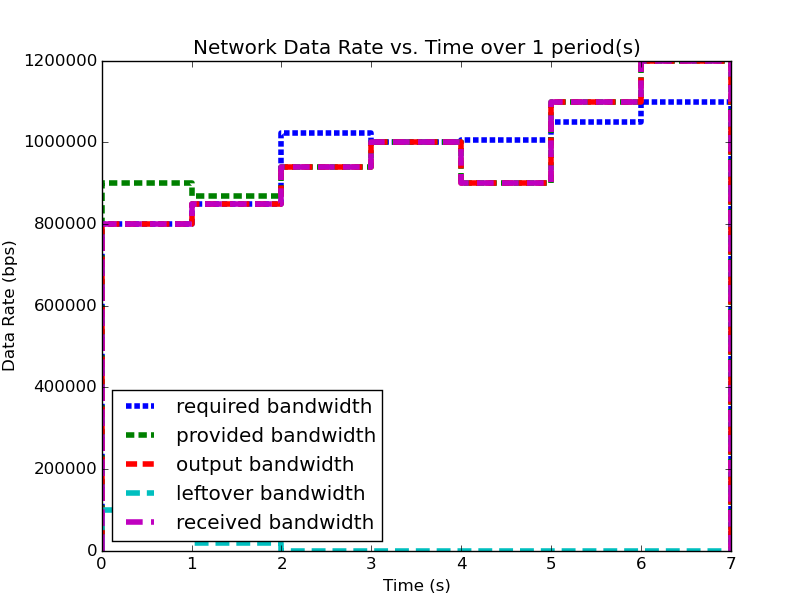
\includegraphics[width=0.8\textwidth]{../doc/src/images/results/1-period-system-bw.png}
  }
  \subfigure[System \emph{(1)} Data for 1 Period]{
    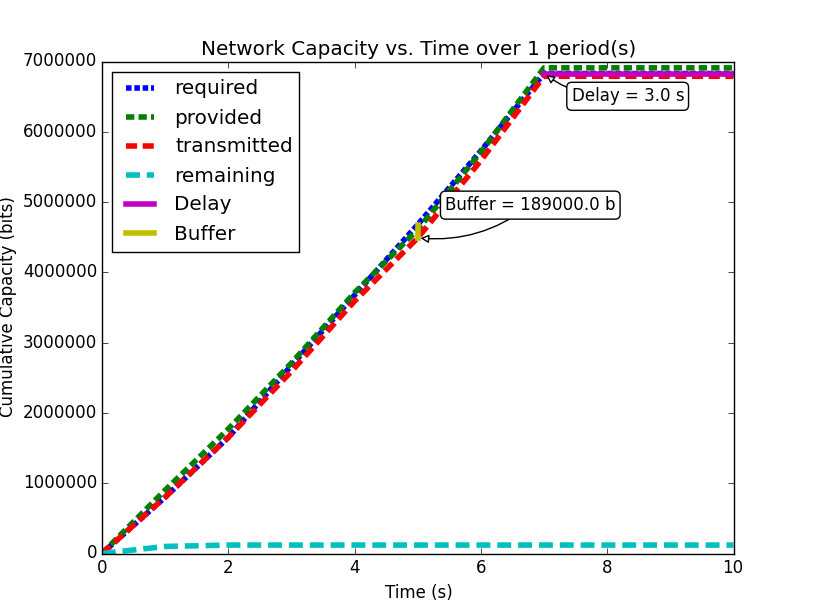
\includegraphics[width=0.8\textwidth]{../doc/src/images/results/1-period-system-data.png}
  }
  \caption{System \emph{(1)} Analyzed over 1 Period}
  \label{fig:1_period_system_1}
\end{figure}

\begin{figure}[ht!]
  \centering
  \subfigure[System \emph{(1)} Data Rate for 2 Periods]{
    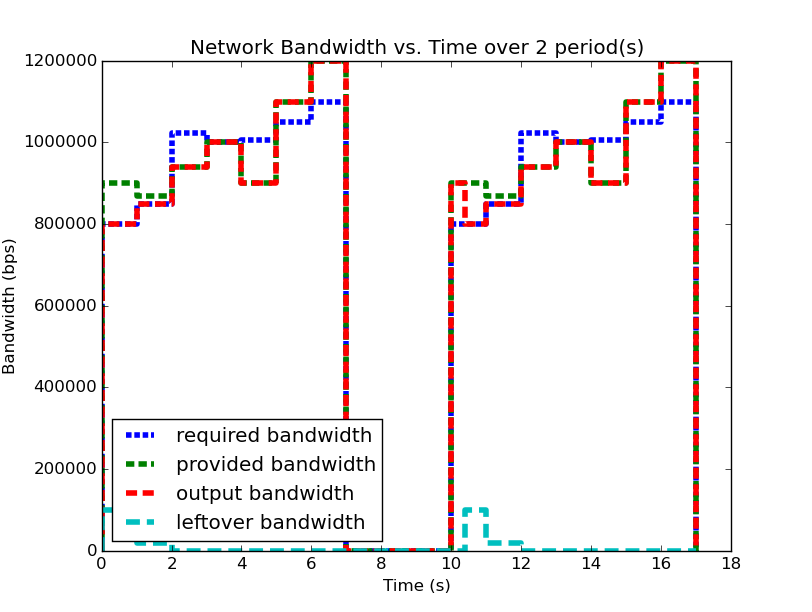
\includegraphics[width=0.8\textwidth]{../doc/src/images/results/2-period-system-bw.png}
  }
  \subfigure[System \emph{(1)} Data for 2 Periods]{
    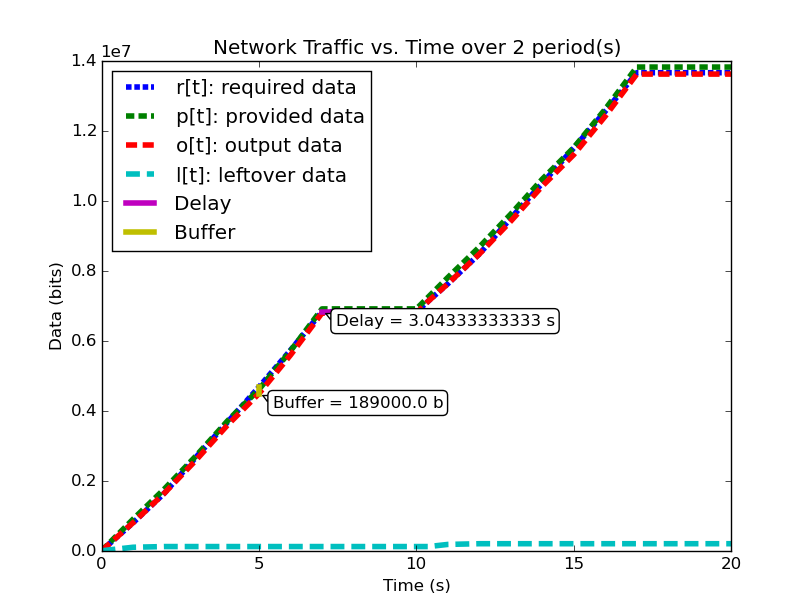
\includegraphics[width=0.8\textwidth]{../doc/src/images/results/2-period-system-data.png}
  }
  \caption{System \emph{(1)} Analyzed over 2 Periods}
  \label{fig:2_period_system_1}
\end{figure}

We notice that for this example system, the second period output
profile is not an exact copy of the first (most easily seen by
examining the bandwidth plots), and yet the required buffer size is
still the same as it was when analyzing the system over one period.
Furthermore, by running the analysis over even larger number of
periods, we can determine (not plotted here for space and
readability), that the predicted buffer size does not change no matter
how many periods we analyze for this system.

Let us look at a system where this is not the case before we begin the
analysis of such system characteristics, shown in
Figure~\ref{fig:1_period_system_2} and Figure~\ref{fig:2_period_system_2}.

\begin{figure}[ht!]
  \centering
  \subfigure[System \emph{(2)} Data Rate for 1 Period]{
    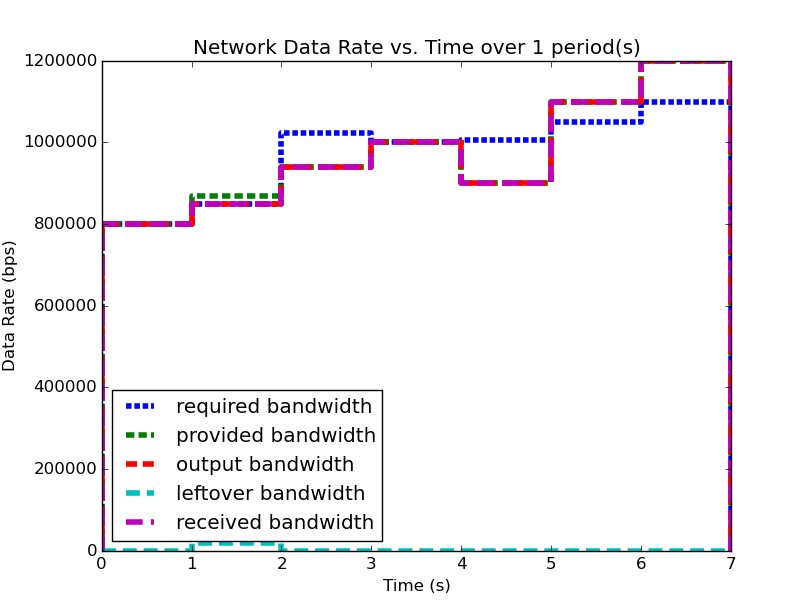
\includegraphics[width=0.8\textwidth]{../doc/src/images/results/1-period-unstable-bw.png}
  }
  \subfigure[System \emph{(2)} Data for 1 Period]{
    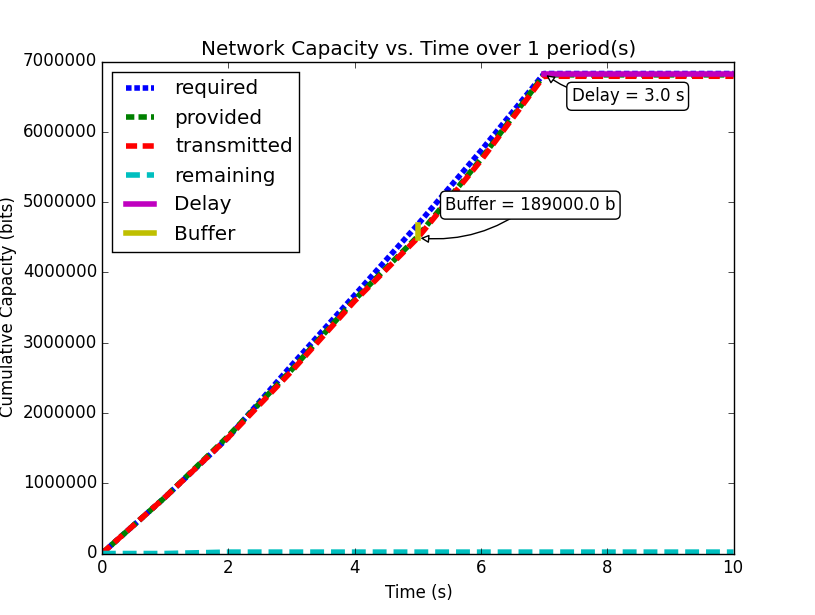
\includegraphics[width=0.8\textwidth]{../doc/src/images/results/1-period-unstable-data.png}
  }
  \caption{System \emph{(2)} Analyzed over 1 Period}
  \label{fig:1_period_system_2}
\end{figure}

\begin{figure}[ht!]
  \centering
  \subfigure[System \emph{(2)} Data Rate for 2 Periods]{
    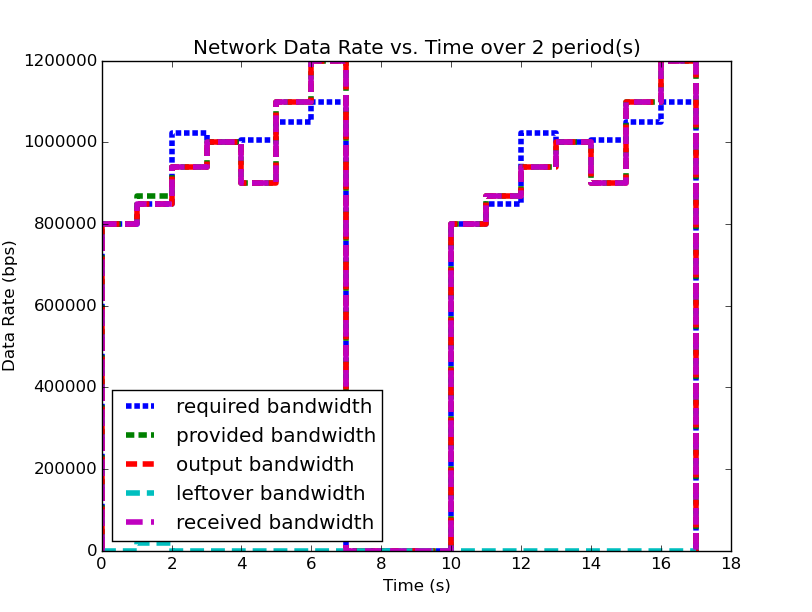
\includegraphics[width=0.8\textwidth]{../doc/src/images/results/2-period-unstable-bw.png}
  }
  \subfigure[System \emph{(2)} Data for 2 Periods]{
    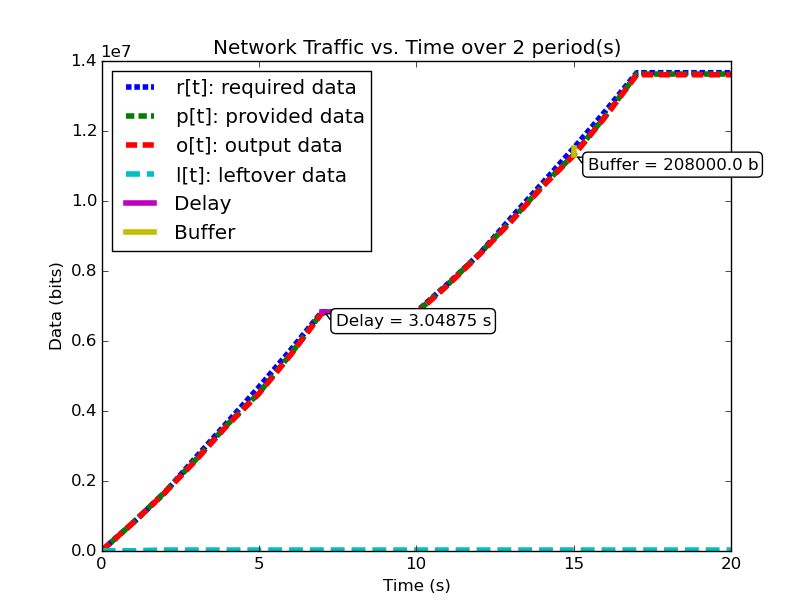
\includegraphics[width=0.8\textwidth]{../doc/src/images/results/2-period-unstable-data.png}
  }
  \caption{System \emph{(2)} Analyzed over 2 Periods}
  \label{fig:2_period_system_2}
\end{figure}

Notice in system \emph{(2)}, the first period analysis predicted the same
buffer size and delay as system \emph{(1)}, but when analyzing two periods
the predicted buffer size changed.  Clearly the behavior of the system
is changing between these two periods.  If we continue to analyze more
periods of system \emph{(2)}, as we did with system \emph{(1)}, we'll find the
unfortunate conclusion that the predicted buffer size increases with
every period we add to the analysis.

We have discovered a system level property that can be calculated from
these profiles, but we must determine what it means and how it can be
used.  First, we see that in system \emph{(1)}, the predicted required
buffer size does not change regarless of the number of periods over
which we analyze the system.  Second, we see that for system \emph{(2)},
the predicted required buffer size changes depending on how many
periods of activity we choose for our analysis window.  Third, we see
that the second period of system \emph{(2)} contains the larger of the two
predicted buffer sizes.  These observations (with our understanding of
deterministic periodic systems) lead us to the conclusion: system
\emph{(2)} can no longer be classified as periodic, since its behavior is
not consistent between its periods.  Furthermore, because the required
buffer size predicted for system system \emph{(2)} continually increases,
we can determine that the system is in fact \emph{unstable} due to
unbounded buffer growth.

\subsection{Proving the Minimum Analysis for System Stability}
\label{subsec:periodic_proof}

Let us now formally prove the assertion about system periodicity and
stability which has been stated above.  We will show that our analysis
results provide quantitative measures about the behavior of the system
and we will determine for how long we must analyze a system to glean
such behaviors.

Typically, periodicity is defined for functions as the equality:

\begin{equation}
  x(t) = x(t + k * T), \forall k \in \mathbb{N} > 0
\end{equation}

but for our type of system analysis this cannot hold since we deal
with cumulative functions (of data vs. time).  Instead we must define
a these functions to be repeating, where a function is repeating
\emph{iff}:

\begin{equation}
  \begin{split}
    x(0) &= 0 \text{  and}\\
    x(t + k * T) &= x(t) + k * x(T), \forall k \in \mathbb{N} > 0
  \end{split}
\end{equation}

Clearly, a repeating function $x$ is \textbf{periodic} \emph{iff}
$x(T)=0$.  Note that repeating functions like the cumulative
data vs. time profiles we deal with, are the result of \textbf{integrating}
\emph{periodic} functions, like the periodic bandwidth vs. time profiles we
use to describe application network traffic and system network
capacity.  All periodic functions, when integrated, produce repeating
functions and similarly, all repeating functions, when differentiated,
procduce periodic functions.

Now we will consider a deterministic, \emph{repeating} queuing system
providing a data service function $S$ to input data function
$I$ to produce output data function $O$, where these
functions are \emph{cumulative data versus time}.  At any time $t$,
the amount of data in the system's buffer is given by $B_t$.
After servicing the input, the system has a remaining capacity
function $R$.

\begin{itemize}
\item $S[t]$ : the service function of the system, cumulative data
  service capacity versus time
\item $I[t]$ : the input data to the system, cumulative data versus
  time
\item $O[t]$ : the output data from the system, cumulative data
  versus time
\item $B[t]$ : the amount of data in the system's buffer at time
  $t$, i.e. $I[t]-O[t]$
\item $R[t]$ : the remaining service capacity of the system after
  servicing $I$, i.e. $S[t] - O[t]$
\end{itemize}

Because $S$ and $I$ are deterministic and repeating, they
increase deterministically from period to period, i.e. given the
period $T_I$ of $I$,

\begin{equation}
  \forall t, \forall n \in \mathbb{N} > 0 : I[t + n*T_I] =
  I[t] + n*I[T_I]
\end{equation}

Similarly, given the period $T_S$ of $S$,

\begin{equation}
  \forall t, \forall n \in \mathbb{N} > 0 : S[t + n*T_S] =
  S[t] + n*S[T_S]
\end{equation}

We can determine the hyperperiod of the system as the $lcm$ of
input function period and the service function period, $T_p =
lcm(T_S,T_I)$.

At the start of the system, $t=0$, the system's buffer is empty,
i.e.  $B[0] = 0$.  Therefore, the amount of data in the buffer
at the end of the first period, $t=T_p$, is the amount of data
that entered the system on input function $I$ but was not able
to be serviced by $S$.  At the start of the next period, this
data will exist in the buffer.  Data in the buffer at the start of the
period can be compared to the system's remaining capacity $R$,
since the remaining capacity of the system indicates how much extra
data it can transmit in that period.  Consider the scenario that the
system's remaining capacity $R$ is less than the size of the
buffer, i.e. $R[T_p] < B[T_p]$.  In this scenario,
$B[2*T_p] > B[T_p]$, i.e. there will be more data in the buffer
at the end of the second period than there was at the end of the first
period.  Since the system is deterministic, for any two successive
periods, $n*T_p$ and $(n+1)*T_p$, $B[n*T_p] >
B[(n+1)*T_p]$, which extends to:

\begin{equation}
   B[m*T_p] > B[n*T_p], \forall m>n>0
\end{equation}

implying that:

\begin{equation}
   B[t] < B[t + k*T_p], \forall k \in \mathbb{N} > 0
\end{equation}

meaning that the amount of data in the buffer versus time is \emph{not
periodic}, therefore the amount of data in the system's buffer
increases every period, i.e. the system has \emph{unbounded buffer growth}.

If however, there is enough remaining capacity in the system to
service the data in the buffer, i.e. $R[T_p] >= B[T_p]$, then
$B[2*T_p] = B[T_p]$.  This relation means that if the remaining
capacity of the system that exists after all the period's required
traffic has been serviced is equal to or larger than the size of the
buffer at the end of the period, then in the next period the system
will be able to service fully both the data in the buffer and the
period's required traffic.  Since both the period's traffic and the
buffer's data will have been serviced in that period, the amount of
data in the buffer at the end of the period will be the same as the
amount of data that was in the buffer at the start of the
period. Similarly to above, since the system is deterministic, for any
two successive periods, $n*T_p$ and $(n+1)*T_p$,
$B[(n+1)*T_p] = B[n*T_p]$.  This extends to:

\begin{equation}
   B[m*T_p] = B[n*T_p], \forall m,n > 0
\end{equation}

which implies that:

\begin{equation}
  B[t] = B[t + k*T_p], \forall k \in \mathbb{N} > 0
\end{equation}

meaning that the amount of data in the buffer versus time is a
\emph{periodic function}, therefore the maximum buffer size does not
grow between periods, and the system has a \emph{finite buffer}.

If we are only concerned with buffer growth, we do not need to
calculate $R$, and can instead infer buffer growth by comparing
the values of the buffer at any two period-offset times during the
steady-state operation of the system ($t >= T_p$).  This means
that the system buffer growth check can resolve to $B[2*T_p] ==
B[T_p]$.  This comparison abides by the conditions above, with
$m=2$ and $n=1$.

\newpage
%%%%%%%%%%%%%%%%%%%%%%%%%%%%%%%%%%%%%%%%%%%%%%%%%%%%%%%%%%%%%%%%%%%%%%%%%%%%%%%%%%%
%%%%%%%%%%%%%%%%%%%%%%%%%%%%%%%%%%%%%%%%%%%%%%%%%%%%%%%%%%%%%%%%%%%%%%%%%%%%%%%%%%%
%%%%%%%%%%%%%%%%%%%%%%%%%%%%%%%%%%%%%%%%%%%%%%%%%%%%%%%%%%%%%%%%%%%%%%%%%%%%%%%%%%%
%%%%%%%%%%%%%%%%%%%%%%%%%%%%%%%%%%%%%%%%%%%%%%%%%%%%%%%%%%%%%%%%%%%%%%%%%%%%%%%%%%%
%%%%%%%%%%%%%%%%%%%%%%%%%%%%%%%%%%%%%%%%%%%%%%%%%%%%%%%%%%%%%%%%%%%%%%%%%%%%%%%%%%%

\section{Comparison of \shorttool/ with Network Calculus}
\label{sec:comparison}

When developing a new analysis technique to predict application
network performance, alternative techniques must be evaluated to
determine the utility of the new techniques.  Application developers
and system integrators can then use these comparisons as a metric for
choosing between the available analysis tools.  For the tools and
techniques to affect a meaningful change in system and application
development, they must be shown to be more effective by some metric
for at least certain classes of systems or applications.

To show how our analysis techniques compare to other available
methods, we developed our tools to allow us to analyze the input
system using Network Calculus/Real-Time Calculus techniques as well as
our own.  Using these capabilities, we can directly compare the
analysis results to each other, and then finally compare both results
to the measurements from an actual system.

\subsection{Results}

Figure~\ref{fig:system_comparison} shows the data rate versus time
profile describing the example system, side-by-side with the
time-integrated and analyzed data versus time profile.
Figure~\ref{fig:zoom_pnp} shows a zoomed in portion of the second
plot, focusing on the area with the maximum delay and buffer as
analyzed by \shorttool/.  Figure~\ref{fig:nc_comparison} shows the
same system analyzed using Network Calculus.

\begin{figure}[ht!]
  \centering
  \subfigure[System Data Rate vs. Time]{
    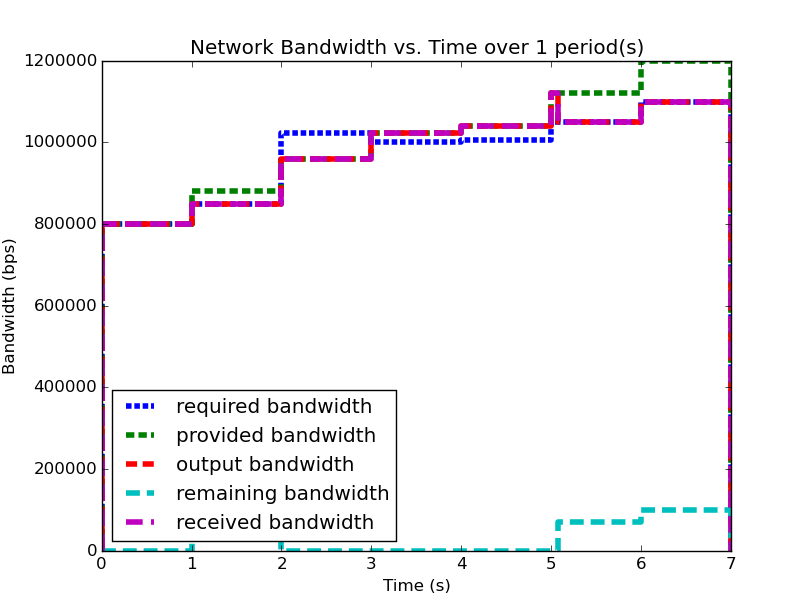
\includegraphics[width=0.8\textwidth]{../doc/src/images/results/maren_namek_bw.png}
  }
  \subfigure[System Data Analyzed with \shorttool/]{
    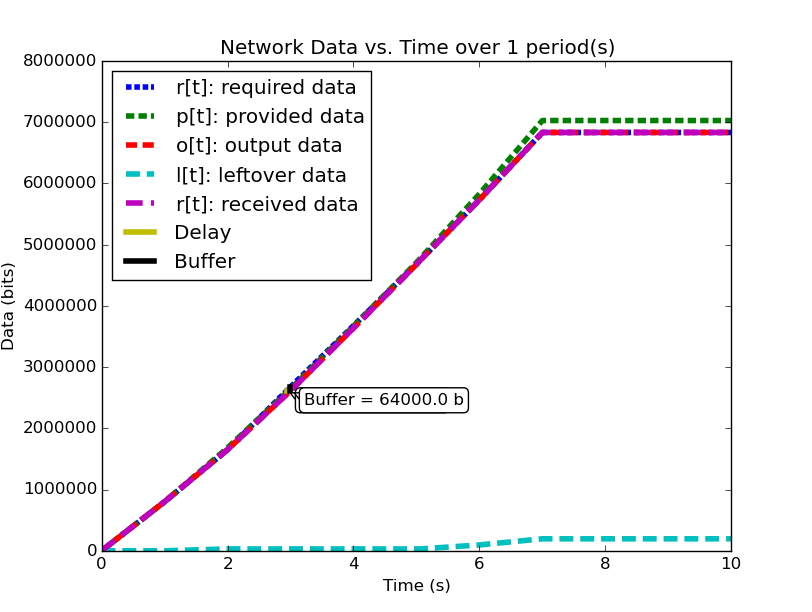
\includegraphics[width=0.8\textwidth]{../doc/src/images/results/maren_namek_data.png}
    \label{subfig:pnp_analysis_comparison}
  }
  \caption{System profile used for comparison of \shorttool/ with
    Network Calculus.  The Analysis using \shorttool/ is shown on the right.}
  \label{fig:system_comparison}
\end{figure}

\begin{figure}[ht!]
  \centering
  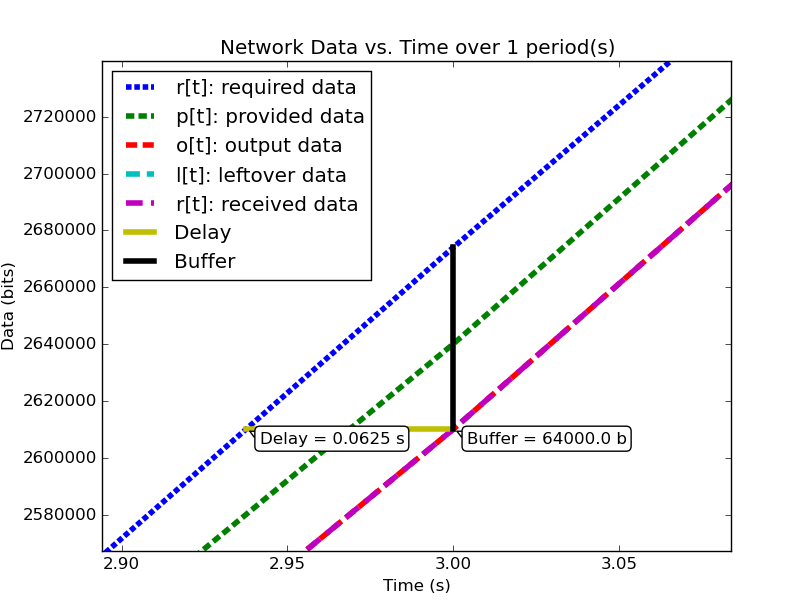
\includegraphics[width=0.85\textwidth]{../doc/src/images/results/maren_namek_data_zoom.png}
  \caption{Zoomed-in verion of
    Figure~\ref{subfig:pnp_analysis_comparison}, focusing on the
    predicted buffer and delay.}
  \label{fig:zoom_pnp}
\end{figure}

\begin{figure}[ht!]
  \centering
  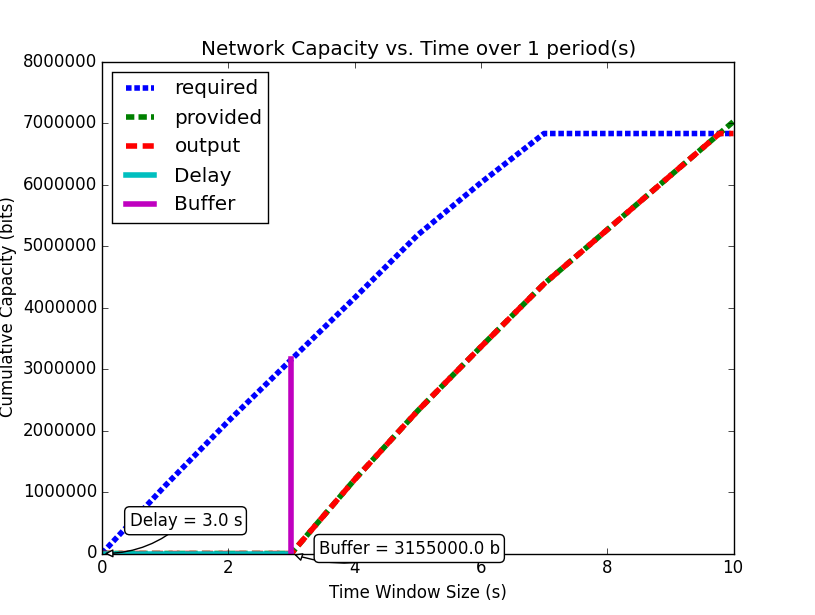
\includegraphics[width=0.85\textwidth]{../doc/src/images/results/nc_namek_data.png}
  \caption{Network-Calculus based analysis of the same system.}
  \label{fig:nc_comparison}
\end{figure}

The major drawback for Network Calculus that our work aims to solve is
the disconnect from the real system that stems from using an approach
based on time-window analysis.  Such an approach leads to dramatically
under-approximating the capacity of the network while simultaneously
over-approximating the utilization of the network, since a known drop
in network performance which is expected and handled by the
application cannot be accurately modeled.  In our case, the system is
using a system profile which can service data during the period from
$0\le t\le 7$ seconds with a period of 10 seconds.  The
application is designed around this constraint and only produces data
during that interval.  Because our technique directly compares when
the application produces data to when the system can service the data,
we are able to derive more precise performance prediction metrics than
Network Calculus, which compares the 3 seconds of system downtime to
the 3 seconds of maximum application data production.

We developed software which produces data according to a supplied
input profile and configured the system's network to provide the
bandwidth profile described in the system configuration profile.
Using this experimental infrastructure, we were able to measure the
transmitted traffic profile, the received traffic profile, the latency
experienced by the data, and the transmitter's buffer requirements.
The results are displayed in the table below:

\begin{table}[htbp]
\caption{Experimental system measurements}
\begin{tabular}{| c | c | c |}
\hline
 & Predicted & Measured ($\mu,\sigma$) \\\hline
Buffer Delay (s) & 0.0625 & (0.06003 , 0.00029) \\\hline
Time of Delay (s) & 3.0 & (2.90547 , 0.00025) \\\hline
Buffer Size (bytes) & 8000 & (7722.59 , 36.94) \\\hline
\end{tabular}
\label{table:results}
\end{table}

Taking the results from our published work, where our methods
predicted a buffer size of 64000 bits, we show that
Network Calculus predicts a required buffer size of 3155000 bits. This
drastic difference comes from the mis-match between down-time and max
data production mentioned above.

\newpage
%%%%%%%%%%%%%%%%%%%%%%%%%%%%%%%%%%%%%%%%%%%%%%%%%%%%%%%%%%%%%%%%%%%%%%%%%%%%%%%%%%%
%%%%%%%%%%%%%%%%%%%%%%%%%%%%%%%%%%%%%%%%%%%%%%%%%%%%%%%%%%%%%%%%%%%%%%%%%%%%%%%%%%%
%%%%%%%%%%%%%%%%%%%%%%%%%%%%%%%%%%%%%%%%%%%%%%%%%%%%%%%%%%%%%%%%%%%%%%%%%%%%%%%%%%%
%%%%%%%%%%%%%%%%%%%%%%%%%%%%%%%%%%%%%%%%%%%%%%%%%%%%%%%%%%%%%%%%%%%%%%%%%%%%%%%%%%%
%%%%%%%%%%%%%%%%%%%%%%%%%%%%%%%%%%%%%%%%%%%%%%%%%%%%%%%%%%%%%%%%%%%%%%%%%%%%%%%%%%%

\section{Analysis of TDMA Scheduling}
\label{sec:tdma}

Medium channel access protocols are used in networking systems to
govern the communication between computing nodes which share a network
communications medium.  They are designed to allow reliable
communication between the nodes, while maintaining certain goals, such
as minimizing network collisions, maximizing bandwidth, or maximizing
the number of nodes the network can handle.  Such protocols include
Time Division Multiple Access (TDMA), which tries to minimize the
number of packet collisions; Frequency Division Multiple Access
(FDMA), which tries to maximize the bandwidth available to each
transmitter; and Code Division Multiple Access (CDMA) which tries to
maximize the number of nodes that the network can
handle\cite{jung1993advantagesCDMAFDMATDMA}.  We will not discuss CDMA
in the scope of this work.

In FDMA, each node of the network is assigned a different transmission
frequency from a prescribed frequency band allocated for system
communications.  Since each node transmits on its own frequency,
collisions between nodes transmitting simultaneously are reduced.
Communications paradigms of this type, i.e. shared medium with
collision-free simultaneous transmission between nodes, can be modeled
easily by our \shorttool/ modeling paradigm described above, since the
network resource model for each node can be developed without taking
into account the transmissions of other nodes.

In TDMA, each node on the network is assigned one or more time-slots
per communications period in which only that node is allowed to
transmit.  By governing these timeslots and having each node agree
upon the slot allocation and communications period, the protocol
ensures that at a given time, only a single node will be transmitting
data, minimizing the number of collisions due to multiple simultaneous
transmitters.  In such a medium access protocol, transmissions of each
node affect other nodes' transmission capability.  Because these
transmissions are scheduled by TDMA, they can be explicitly integrated
into the system network resource model.

\subsection{Problem}
TDMA transmission scheduling has an impact on the timing
characteristics of the applications' network communications.  Because
applications' network data production is decoupled from their node's
TDMA transmission time slot, buffering may be required when an
application on one node tries to send data on the network during the
transmission slot of a different node.  In this case, the data would
need to be buffered on the application's node and would therefore
incur additional buffering delay.  If this TDMA schedule is not
integrated into the analysis of the network resources, the additional
buffer space required may exceed the buffer space allocation given to
the application or the buffering delay may exceed the application's
acceptable latency.

\subsection{Results}

So far, the description of the system provided network service profile
($p[t]=y$), has been abstracted as simply the available
bandwidth as a function of time integrated to produce the amount of
data serviced as a function of time. We show how to model and analyze
the network's lower-level TDMA MAC protocol using our network modeling
semantics.  We then derive general formulas for determining the affect
TDMA has on buffer size and delay predictions.

As an example TDMA system which benefits from our analysis techniques,
consider an application platform provided by a fractionated satellite
cluster.  For this system, the network between these satellites is a
precious resource shared between each of the applications' components
in the cluster.  To ensure the stability of the network resources,
each satellite has a direct connection to every other satellite and is
assigned a slot in the TDMA schedule during which the satellite may
transmit.  Each TDMA slot has a sinusoidally time-varying bandwidth
profile which may differ from the other TDMA slot bandwidth profiles.
The time-varying profile of the slot bandwidth comes from the coupling
between the radios' inverse-squared
bandwidth-as-a-function-of-distance and the satellites' sinusoidal
distance-as-a-function-of-orbital-position, as described in
Section~\ref{sec:intro}. The requirement for accurate performance
prediction necessitates the incorporation of the TDMA schedule into
the network modeling and analysis.

TDMA schedules can be described by their period, their number of
slots, and the bandwidth available to each slot as a function of time.
For simplicity of explanation, we assume that each node only gets a
single slot in the TDMA period and all slots have the same length, but
the results are valid for all static TDMA schedules.  Note that each
slot still has a bandwidth profile which varies as a function of time
and that each slots may have a different bandwidth profile.

In a given TDMA period $T$, a node $n$ can transmit a certain number
of bits governed by its slot length $t_{n}$ and the slot's available
bandwidth $bw_{n}$.  During the rest of the TDMA period, the node's
available bandwidth is $0$.  This scheduling has the effect of
amortizing the node's slot bandwidth into an effective bandwidth of
$bw_{effective}$.  The addition of the TDMA scheduling can affect the
buffer and delay calculations, based on the slot's bandwidth, the
number of slots, and the slot length.  The maximum additional delay is
$\Delta_{delay}$, and the maximum additional buffer space is
$\Delta_{buffer}$.  These deviations are shown graphically by
Figure~\ref{fig:tdma} and calculated by
\begin{equation}
  \begin{split}
    bw_{effective} &= bw_{n} * \dfrac{t_n}{T}\\
    \Delta_{delay} &= T - t_{n}\\
    \Delta_{buffer} &= \Delta_{delay} * bw_{effective}
  \end{split}
  \label{eq:tdma}
\end{equation}
Where:
\begin{itemize}
\item $T$ is the period of the TDMA schedule
\item $t_n$ is the length of node $n$'s TDMA slot
\item $bw_n$ is the bandwidth available to node $n$ during its slot
\item $bw_{effective}$ is the perceived bandwidth available to the
  node during the TDMA period
\item $\Delta_{delay}$ is the change in the predicted delay
  experienced by application traffic on the network
\item $\Delta_{buffer}$ is the change in the predicted buffer space
  required for lossless transmission of application traffic
\end{itemize}
Clearly, $\Delta_{delay}$ is bounded by $T$
and $\Delta_{buffer}$ is governed by $t_{n}$.  Therefore, because
$t_{n}$ is dependent on $T$, minimizing $T$ minimizes both the maximum
extra delay and maximum extra buffer space.
\begin{figure}[ht!]
  \centering
  \subfigure[In-Phase TDMA Profile vs Abstract]{
    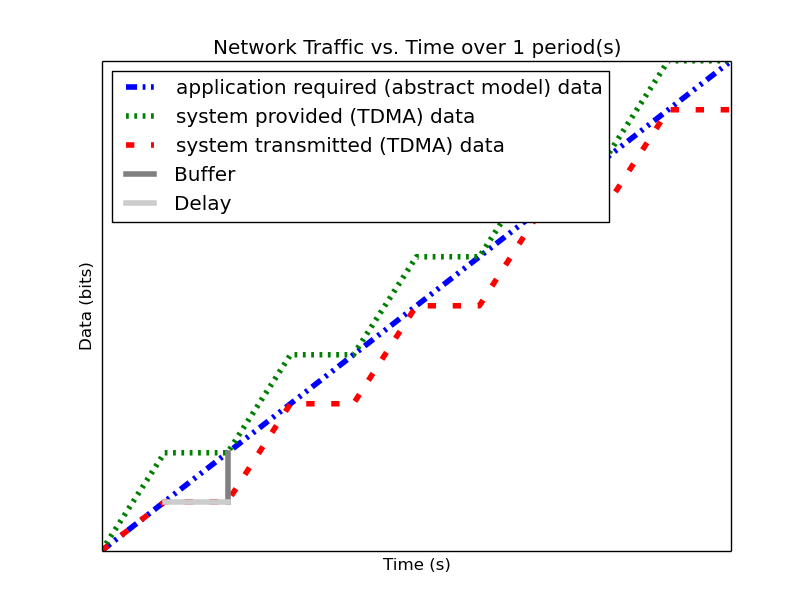
\includegraphics[width=0.8\textwidth]{../doc/src/images/results/tdma_phase0.png}
  }
  \subfigure[Out-of-Phase TDMA Profile vs Abstract]{
    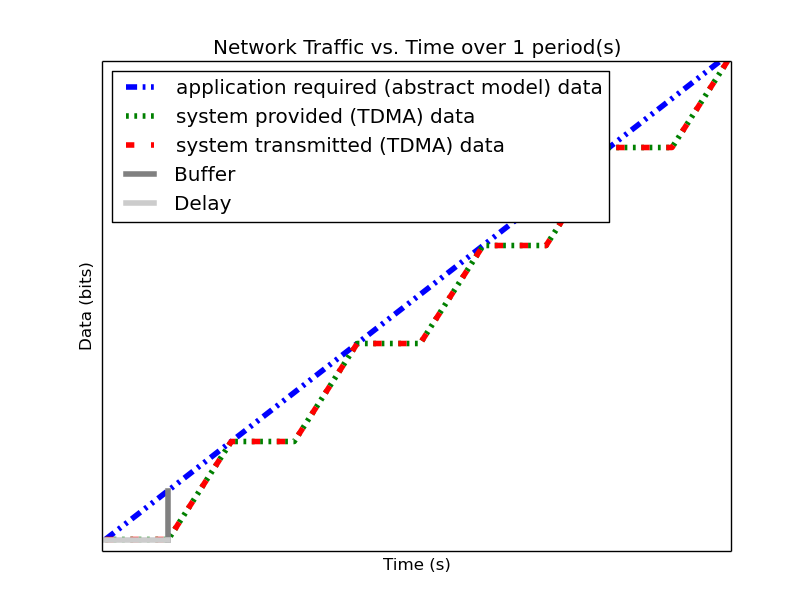
\includegraphics[width=0.8\textwidth]{../doc/src/images/results/tdma_phase1.png}
  }
  \caption{Effects of TDMA scheduling in the MAC layer on system
    network performance.}
  \label{fig:tdma}
\end{figure}

Following from this analysis, we see that if: (1) the TDMA effective
bandwidth profile is provided as the abstract system network service
profile, and (2) the TDMA period is much smaller than the duration of
the shortest profile interval; then the system with explicit modeling
of the TDMA schedule has similar predicted application network
characteristics as the abstract system.  Additionally, the maximum
deviation formulas derived above provide a means for application
developers to analyze the their application on a TDMA system without
explicitly integrating the TDMA model into the system profile model.

Through the analysis of TDMA scheduling's effect on application level
performance prediction, we derived analytical formulas for the maximum
deviation between the abstract system model and the model with
explicitly encoded TDMA scheduling.  The use of these formulas frees
developers and system integrators from having to explicitly
incorporate the TDMA schedule in their application and system models.
This TDMA modeling and analysis was published in
\cite{ISIS_F6_ISORC_QOS:15}.

\newpage
%%%%%%%%%%%%%%%%%%%%%%%%%%%%%%%%%%%%%%%%%%%%%%%%%%%%%%%%%%%%%%%%%%%%%%%%%%%%%%%%%%%
%%%%%%%%%%%%%%%%%%%%%%%%%%%%%%%%%%%%%%%%%%%%%%%%%%%%%%%%%%%%%%%%%%%%%%%%%%%%%%%%%%%
%%%%%%%%%%%%%%%%%%%%%%%%%%%%%%%%%%%%%%%%%%%%%%%%%%%%%%%%%%%%%%%%%%%%%%%%%%%%%%%%%%%
%%%%%%%%%%%%%%%%%%%%%%%%%%%%%%%%%%%%%%%%%%%%%%%%%%%%%%%%%%%%%%%%%%%%%%%%%%%%%%%%%%%
%%%%%%%%%%%%%%%%%%%%%%%%%%%%%%%%%%%%%%%%%%%%%%%%%%%%%%%%%%%%%%%%%%%%%%%%%%%%%%%%%%%

\section{Compositional Analysis}
\label{sec:compositional_analysis}

Now that we have precise network performance analysis for aggregate
profiles or singular profiles on individual nodes of the network, we
must determine how best to compose these profiles and nodes together
to analyze the overall system.  The aim of this work is to allow the
profiles from each application to be analyzed separately from the
other profiles in the network, so that application developers and
system integrators can derive meaningful perfomance predictions for
specific applications.  For this goal, let us define:

\begin{definition}[Compositionality]\cite{sifakis2002}
  A system is compositional if its properties can be derived from
  the properties of its components and how they are interconnected.
\end{definition}

\begin{definition}[Composability]\cite{sifakis2002}
  A component is composable if its properties do not change
  when the component is composed with other components.
\end{definition}

For our analysis techniques to be compositional, an application's
required profile must be analyzable individually without requiring
aggregation with the rest of the required profiles in the system.
This means that the system's performance, i.e. the peformance of all
the applications on the system, can be determined by analyzing the
performance of each application individually.

To achieve compositionality, we must not only define mathematical
operations which allow us to aggregate and separate profiles with/from
each other, but also the semantics of how these profiles are composed
with one another.  This semantics govern the relation between
required profiles, specifically governing the distribution of their
shared node's provided profile between each other.  For our
compositional analysis, we defined that each required profile in the
system be given a unique priority, $U$, with the relation that a
profile $P_1$ has a higher priority than profile $P_2$
\emph{iff} $U_{P_1} < U_{P_2}$.  Using this priority relation, we can
define that a profile $P_i$ does not receive any capacity from
its node at time $t$ until all other profiles with priority
$< U_{P_i}$ have received their requested capacity from the
node at $t$.  If the node does not have enough capacity at
$t$ to service $P_i$, then the data $P_i$ attempted
to send at $t$ will be placed into its buffer, to be sent at a
time when the node has available bandwidth for $P_i$.

This priority relation for compositional analysis is similar to the
task priority used for schedulability analysis in Real-Time Calculus,
mentioned in :ref:$rtc$.  Similarly to RTC, this priority relation and
compositionality allow us to capture the effects independent profiles
have on each other when they share the same network resources.  Just
as RTC based its priority relation and computation scheduling on a
fixed-priority scheduler, our priority relation and resource allotment
is based on the network Quality-of-Service (QoS) management provided
by different types of networking infrastructure.  One such mechanism
for implementing this type of priority-based network resource
allocation is through the use of the DiffServ Code Point
(DSCP)\cite{rfc2474}.  The DSCP is a bit-field in all packets which
have an Internet Protocol (IP) header which allows the packet to be
assigned a specific class for per-hop routing behavior.  Routers and
forwarders in the network group packets according to their DSCP class
and provide different service capacities to each class.  For example,
the \emph{Expedited Forwarding} \cite{rfc3246} class receives strict
priority queuing above all other traffic, which makes it a suitable
implementation of this type of resource allocation.  Similarly, the
Linux Traffic Control\cite{linux_tc} utility provides many mechanisms
for shaping, policing, routing, and classifying traffic.  Its
class-based queuing disciplines and filtering mechanisms provide the
capability for such strict priority-based network resource
allocation.  

Mathematically, compositionality requires that we be able to add and
subtract profiles from each other, for instance to determine the
remaining service capacity of a node available for a profile $P_i$
after it serves all profiles with a higher priority.  Queuing of the
lower priority profiles is taken into account when the lower priorty
profile is convolved with the remaining capacity the node has
available to service it.  The calculation of the remaining capacity,
$P_P'$, of the node after it services $P_i$ is given as:
\begin{equation}
  P_P' = P_P - ( P_i \otimes P_P )
\end{equation}
Where
\begin{itemize}
\item $P_P$ is the capacity available to profile $P_i$
\end{itemize}

Mathematically, addition and subtraction of two profiles $f[t],g[t]$ is given by:
\begin{equation}
  \begin{split}
    \dot s[t] &= \dot f[t] + \dot g[t]\\
    s[t] &= \int_{0}^t\dot s[\tau]d\tau
  \end{split}
\end{equation}
and
\begin{equation}
  \begin{split}
    \dot s[t] &= \dot f[t] - \dot g[t]\\
    s[t] &= \int_{0}^t\dot s[\tau]d\tau
  \end{split}
\end{equation}
meaning that addition and subtraction are performed on the data rate
representations of the profiles, which are periodic functions of time.

Experimental validation of these compositional techniques,
specifically with respect to priority relation, adding, and
subtracting of profiles is presented at the end of
Section~\ref{sec:routing}.

\newpage
%%%%%%%%%%%%%%%%%%%%%%%%%%%%%%%%%%%%%%%%%%%%%%%%%%%%%%%%%%%%%%%%%%%%%%%%%%%%%%%%%%%
%%%%%%%%%%%%%%%%%%%%%%%%%%%%%%%%%%%%%%%%%%%%%%%%%%%%%%%%%%%%%%%%%%%%%%%%%%%%%%%%%%%
%%%%%%%%%%%%%%%%%%%%%%%%%%%%%%%%%%%%%%%%%%%%%%%%%%%%%%%%%%%%%%%%%%%%%%%%%%%%%%%%%%%
%%%%%%%%%%%%%%%%%%%%%%%%%%%%%%%%%%%%%%%%%%%%%%%%%%%%%%%%%%%%%%%%%%%%%%%%%%%%%%%%%%%
%%%%%%%%%%%%%%%%%%%%%%%%%%%%%%%%%%%%%%%%%%%%%%%%%%%%%%%%%%%%%%%%%%%%%%%%%%%%%%%%%%%

\section{Delay Analysis}
\label{sec:delay}

When dealing with queueing systems (esp. networks) where precise
design-time guarantees are required, the delay in the links of the
network must be taken into account.

The delay is modeled as a continuous function of latency (seconds)
versus time.  In the profiles, the latency is specified discretely as
$(time, latency)$ pairs, and is interpolated linearly between
successive pairs.  Specifically, $time$ is a time point at which the
latency on the link is given by $latency$.  

Using this latency semantics, the delay convolution of a profile
becomes

\begin{equation}
  r[t + \delta[t]] = l[t]
\end{equation}

Where

\begin{itemize}
\item $l[t]$ is the \emph{link} profile describing the data as a
  function of time as it enters the link
\item $\delta[t]$ is the \emph{delay} profile describing the latency
  as a function of time on the link
\item $r[t]$ is the \emph{received} profile describing the data as a
  function of time as it is received at the end of the link
\end{itemize}
  
When analyzing delay in a periodic system, it is important to
determine the effects of delay on the system's periodicity.  We know
that the period of the periodic profiles is defined by the time
difference between the start of the profile and the end of the
profile.  Therefore, we can show that if the time difference between
the \textbf{start time} of the \emph{received} profile and the
\textbf{end time} of the \emph{received} profile is the same as the
\textbf{period} of the \emph{link} profile, the periodicity of the
profile is unchanged.

\begin{itemize}
\item $T_p$ is the period of the \emph{link} profile
\item $r[t + \delta[t]]$ is the beginning of the \emph{received}
  profile
\item $r[(t + T_p) + \delta[(t + T_p)]]$ is the end of the
  \emph{received} profile
\end{itemize}

We determine the condition for which $(t_{end}) - (t_{start}) =
T_p$:

\begin{equation}
  \begin{split}
    (T_p + t + \delta[T_p + t]) - (t + \delta[t]) &= T_p \\
    T_p + \delta[T_p + t] - \delta[t] &= T_p \\
    \delta[T_p + t] - \delta[t] &= 0\\
    \delta[T_p + t] &= \delta[t]
  \end{split}
\end{equation}

Which is just confirms that the periodicity of the delayed profile is
unchanged \emph{iff} the latency profile is \textbf{periodic}, i.e.

\begin{equation}
\delta[t] = \delta[t + k*T_p], \forall k\in\mathbb{N} > 0
\end{equation}

Experimental validation of this delay analysis is presented at the end
of Section~\ref{sec:routing}.

\newpage
%%%%%%%%%%%%%%%%%%%%%%%%%%%%%%%%%%%%%%%%%%%%%%%%%%%%%%%%%%%%%%%%%%%%%%%%%%%%%%%%%%%
%%%%%%%%%%%%%%%%%%%%%%%%%%%%%%%%%%%%%%%%%%%%%%%%%%%%%%%%%%%%%%%%%%%%%%%%%%%%%%%%%%%
%%%%%%%%%%%%%%%%%%%%%%%%%%%%%%%%%%%%%%%%%%%%%%%%%%%%%%%%%%%%%%%%%%%%%%%%%%%%%%%%%%%
%%%%%%%%%%%%%%%%%%%%%%%%%%%%%%%%%%%%%%%%%%%%%%%%%%%%%%%%%%%%%%%%%%%%%%%%%%%%%%%%%%%
%%%%%%%%%%%%%%%%%%%%%%%%%%%%%%%%%%%%%%%%%%%%%%%%%%%%%%%%%%%%%%%%%%%%%%%%%%%%%%%%%%%

\section{Analysis of Statically Routed Networks}
\label{sec:routing}

\subsection{Problem}
As CPS become more distributed in nature and begin to act as
infrastructure for distributed applications towards IoT systems, they
will necessarily need to handle more network resource management and
network connection routing within their network as well as between
their own network and any external networks to which they are
connected.  Such networks generally rely on routing to allow more
flexibility in the system with respect to node placement and
connectivity.  Adding routing to the network also has the effect of
increasing the complexity of the network performance analysis and can
cause drastic differences in application network performance when
compared with networks without routing.  Therefore the design-time
analysis tools which help predict application network performance must
take this routing into account.  It should be noted that this is a
special case of routing in ad-hoc networks, where one or more nodes
can route messages for other nodes.

\subsection{Results}
Having discussed profile composition and the affects of delaying a
profile, we can address one more aspect of system analysis:
\emph{routing}.  For this analysis we will specifically focus on
statically routed networks.

Firstly, we must define the assumptions we make about the router nodes
with respect to how they forward the network traffic.  In our modeling
and analysis, because we have not considered transmission
error/corruption, we are most closely modeling cut-through routing /
wormhole switching in which the routing and forwarding nodes in the
system forward all packets without checking them for corruption or
integrity.  This forwarding mechanism differs from store and forward
routing in which each packet is checked for errors in its entirety
before sending it to the next node on its route.  In the case of store
and forward, when a corrupt packet is received by a routing node, it
will not forward that packet along its path, and may optionally
request retransmission of the packet from the previous node.  Under
the assumption of no transmission errors, we can incorporate the added
latency incurred by store and forward into the latency profile of the
router node.  In this way, these two forwarding techniques can be
modeling in a simple way using our semantics (where they both simply
affect the latency of the node).  

Given these assumptions about the forwarding techniques of the routing
nodes, we can describe system-level analysis.  By incorporating both
the latency analysis with the compositional operations we developed,
we can perform system-level analysis of profiles which are routed by
nodes of the system.  In this paradigm, nodes can transmit/receive
their own data, i.e. they can host applications which act as data
sources or sinks, as well as act as routers for profiles from and to
other nodes.  To make such a system amenable to analysis we must
ensure that we know the routes the profiles will take at design time,
i.e. the routes in the network are static and known or calculable.
Furthermore, we must, for the sake of profile composition as decribed
above, ensure that each profile has a priority that is unique within
the network which governs how the transmitting and routing nodes
handle the profile's data.

Let us define the system configuration $C$ as:

\begin{equation}
  C = \{\{P_S\},\{N\},\{R\}\}
\end{equation}

Where

\begin{itemize}
\item $\{P_S\}$ is the \emph{set} of all \emph{sender} profiles in the system
  configuration
\item $\{N\}$ is the \emph{set} of all \emph{nodes} in the system configuration, and
\item $\{R\}$ is the \emph{set} of all \emph{routes} in the system configuration
\end{itemize}

We define a profile $P$ as:

\begin{equation}
  P = \{N_I,K,T,F,U,\{(t,R_D,D,L)\}\}
\end{equation}

Where

\begin{itemize}
\item $N_I$ is the \emph{Node ID} to which the profile applies
\item $K$ is the \emph{kind} of the profile, where
  $K\in\{provided,required,receiver\}$
\item $T$ is the \emph{period} of the profile
\item $F$ is the \emph{flow ID} of the profile, where two profiles,
  $P_1,P_2$ belong to the same flow \emph{iff}
  $F_{P_1}==F_{P_2}$
\item $U$ is the \emph{priority} of the profile, where profile
  $P_1$ has a higher priority than profile $P_2$ \emph{iff}
  $U_{P_1} < U_{P_2}$, and
\item $\{(t,R_D,D,L)\}$ is a \emph{set} of $(time, data\ rate,
  data, latency)$ tuples describing how each of $\{data\ rate,
  data, latency\}$ vary with respect to time.  Semantically, the
  $data\ rate$ is constant between any two successive values of
  $t$, while the $data$ and $latency$ are \emph{linearly
  interpolated} during the same interval.  The initial profile
  specification does not have the $data$ field; $data$ is
  calculated based on $data\ rate$.
\end{itemize}

Then we define a node $N$ as:

\begin{equation}
  N = \{I,P_P,\{P_R\}\}
\end{equation}

Where 

\begin{itemize}
\item $I$ is the \emph{ID} of the node
\item $P_P$ is the \emph{provided} profile of the node, and
\item $\{P_R\}$ is the \emph{set} of all \emph{receiver} profiles on the node
\end{itemize}

And finally, we define a route $R$ as:

\begin{equation}
  R = \{N_{I_1},N_{I_2},...,N_{I_N}\}
\end{equation}

Where

\begin{equation}
  \forall N_X,N_Y \subset N, \exists! R_{X,Y} = \{N_{I_X},...,N_{I_Y}\}
\end{equation}

We can then run Algorithm~\ref{lst:routing_alg} to iteratively analyze
the system.  In this algorithm, the remaining capacity of the node is
provided to each profile with a lower priority iteratively.  Because
of this iterative recalculation of node provided profiles based on
routed profiles, we directly take into account the effect of multiple
independent profiles traversing the same router; the highest priority
profile receives as much bandwidth as the router can give it, the next
highest priority profile receives the remaining bandwidth, and so on.

\begin{listing}[ht!]
  \begin{minted}{python}
  analyze( sender_profiles )
  {
    sender_profiles = sorted(sender_profiles, priority)
    for required_profile in sender_profiles
    {
      transmitted_nodes = list.empty() 
      for receiver_profile in
          required_profile.receiver_profiles()
      {
        route =
          getRoute(required_profile, receiver_profile)
        for node in route
        {
          if node in transmitted_nodes
            and multicast == true
	  {
	    continue
	  }
	  provided_profile = node.provided_profile
            
	  output_profile =
            convolve(required_profile, provided_profile)
	  remaining_profile =
            provided_profile - output_profile
	  received_profile =
            delay(output_profile, provided_profile)
            
	  node.provided_profile = remaining_profile
	  required_profile = received_profile
	  transmitted_nodes.append(node)
        }
        receiver_received_profile =
          convolve(required_profile, receiver_profile)
      }
    }
  }
  \end{minted}
  \caption{Algorithm for iteratively analyzing profiles in a
    distributed system with static routing and profile priorities.}
  \label{lst:routing_alg}
\end{listing}

We take care of matching all senders to their respective receivers,
and ensure that if the system supports multicast, a no retransmissions
occur; only nodes which must route the profile to a new part of the
network retransmit the data.  However, if the system does not support
multicast, then the sender must issue a separate transmission, further
consuming network resources.  In this way, lower-level transport
capabilities can be at least partially accounted for by our analysis.

We have implmented these functions for statically routed network
analysis into our tool, which automatically parses the profiles, the
network configuration and uses the algorithm and the implemented
mathematics to iteratively analyze the network.  Analytical results
for example systems will be provided when the experimental results can
be used as a comparison.

To determine the validity of our routing, composition, and delay
analysis, we developed a sample system and application deployment
consisting of two flows generated by two profiles, one a high priority
flow and one a low priority flow.  Each flow originates on a separate
computing node, with different destinations.  Both flows are routed
through the same routing node that enforces priority-based routing for
the two flows.  Figure~\ref{fig:routing_example} shows the
configuration of the system and application for the experimental
validation of the routing, composition, and delay analysis techniques.

\begin{figure}[ht!]
  \centering
  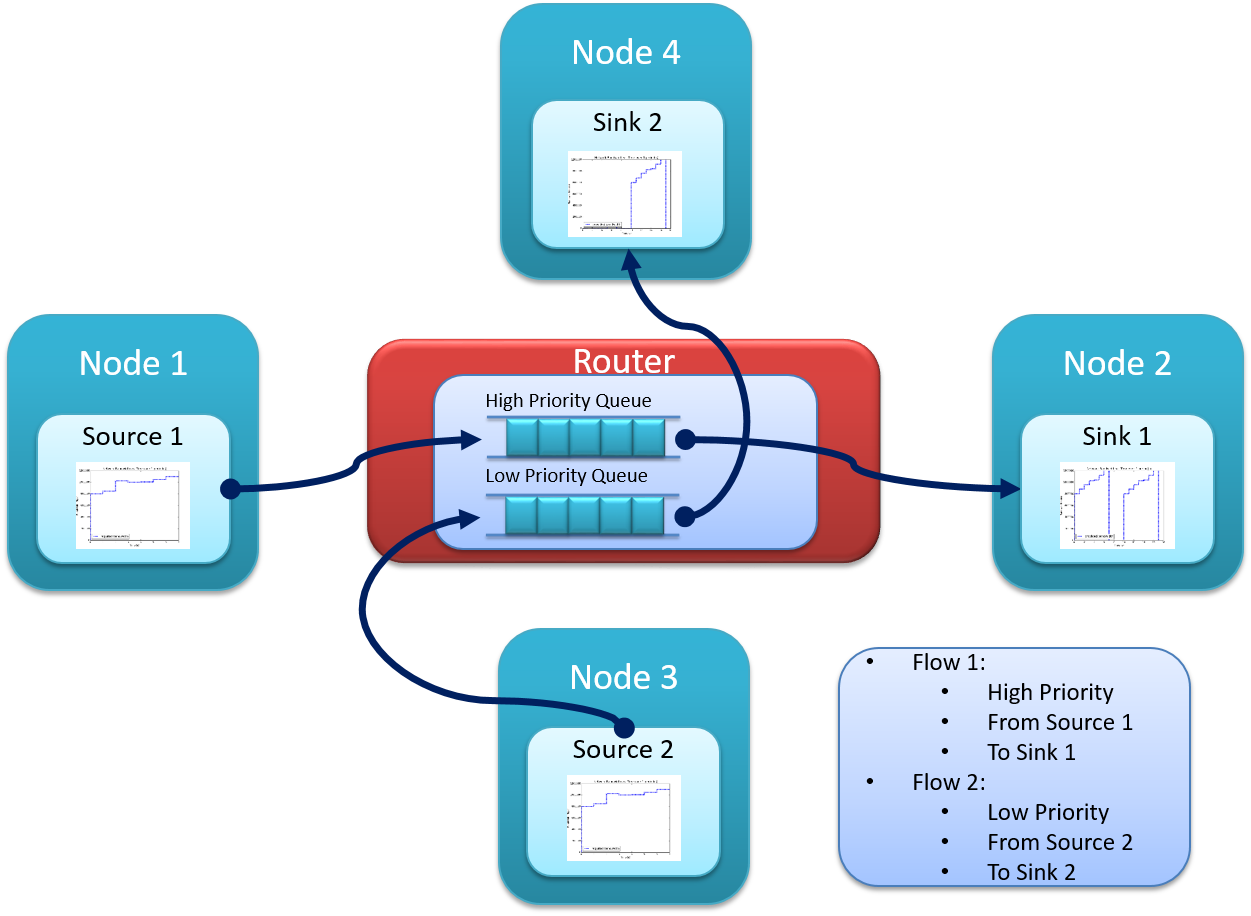
\includegraphics[width=\textwidth]{../doc/src/images/results/routing_example.png}
  \caption{Experimental setup to validate routing, delay, and
    compositional analysis of network profiles.}
  \label{fig:routing_example}
\end{figure}

We configure the system's routing, network delay, and network
bandwidth capacity using Linux's built-in Traffic Control
(TC)\cite{linux_tc} tool, which allows for the configuration of static
routing, heirarchical class-based traffic scheduling, and traffic
shaping.  We configured the output interfaces on each node as
a combination of two queueing disciplines (qdiscs): 1) a network
emulator (netem) which enforces the link delay, and 2) a token-bucket
filter (TBF) which enforces the rate control to enforce the link's
bandwidth profile.  On the routing node, we added an additional
priority qdisc (prio), with multiple priority queues.  We configured
TC to filter packets into these queues by matching packet source IP
address and destination IP address.  This filtering ensured that the
high priority flow's packets would be filtered into the high-prioirty
queue of the prio qdisc, while the lower priority flow's packets would
be filtered into the lower priority queue of the prio qdisc.  All
traffic out of the priority qdisc was fed into the TBF to ensure that
all traffic, regardless of priority, shared and was shaped by the
node's link capacity profile.  

This experimental setup allows us to examine the validity of our
analysis techniques in the following ways:

\begin{itemize}
  \item Because the system implements the strict priority queueing of
    flows, especially independent interacting flows, we can compare
    the delay and buffering measurements to the same delay and buffer
    predictions from the model.
  \item Router buffer space requirements can be measured and compared
    with their predicted requirements to validate routed network
    analysis.
  \item Link delay composition can be validated by examining the
    receiver buffer requirements compared with the predicted receiver
    buffer sizes.  
\end{itemize}

\iffalse
Using this system and application configuration, we can validate the
analysis results by comparing:

\begin{itemize}
  \item The delay measured between the reception of data and
    transmission of data \emph{versus} the predicted delay
  \item The buffer measured between on the receiver end of the data
    flow \emph{versus} the predicted receiver buffer size for each flow
\end{itemize}

Additionally, the analysis techniques are useful for predicting the
required buffer size on the routing node for each of the queues
corresponding to the two flows.  Because we can directly control the
size of these queues, we can show that if we configure their sizes to
be the analysis' predicted sizes and we lose no messages then the
predicted buffer sizes are sufficient for the system and application
configuration.  
\fi

The results of our experiments using this application and system
configuration are shown in Table~\ref{table:routing_results}.

\begin{table}[htbp]
\caption{Delay and Buffer Results: Prediction versus Experiment for
  Routing Analysis. TO BE FILLED OUT WHEN DATA IS AVAILABLE}
\begin{tabular}{| c | c | c |}
\hline
 & Predicted & Measured ($\mu,\sigma$) \\\hline
Buffer Delay (s) & 0.0625 & (0.06003 , 0.00029) \\\hline
Time of Delay (s) & 3.0 & (2.90547 , 0.00025) \\\hline
Buffer Size (bytes) & 8000 & (7722.59 , 36.94) \\\hline
\end{tabular}
\label{table:routing_results}
\end{table}

We are finishing the design and development of code which will allow
us to run experiments to validate our routing analysis results.  They
will be complete in the next two weeks.



\iffalse

\newpage
%%%%%%%%%%%%%%%%%%%%%%%%%%%%%%%%%%%%%%%%%%%%%%%%%%%%%%%%%%%%%%%%%%%%%%%%%%%%%%%%%%%
%%%%%%%%%%%%%%%%%%%%%%%%%%%%%%%%%%%%%%%%%%%%%%%%%%%%%%%%%%%%%%%%%%%%%%%%%%%%%%%%%%%
%%%%%%%%%%%%%%%%%%%%%%%%%%%%%%%%%%%%%%%%%%%%%%%%%%%%%%%%%%%%%%%%%%%%%%%%%%%%%%%%%%%
%%%%%%%%%%%%%%%%%%%%%%%%%%%%%%%%%%%%%%%%%%%%%%%%%%%%%%%%%%%%%%%%%%%%%%%%%%%%%%%%%%%
%%%%%%%%%%%%%%%%%%%%%%%%%%%%%%%%%%%%%%%%%%%%%%%%%%%%%%%%%%%%%%%%%%%%%%%%%%%%%%%%%%%

\section{Application Network Profile Generation from Business Logic Models}
\label{sec:generation}

Let us consider a platform that consists of a set of computing nodes,
each node equipped with a number of hardware devices. The nodes are
connected to each other over an ad-hoc, dynamic communication network.
We consider a subset of distributed software platforms, where the
applications are integrated from prefabricated components. A component
is the basic unit in the system that can provide a functionality. It
interacts with other components using well-defined interaction
patterns. Component-based software engineering has been extensively
applied to distributed real-time applications
~\cite{Emb_SW_PECOS:02,RT_CIAO:04,PROGRESS_ICSEA:08,ACM_SPE:10,ISIS_F6_ISORC:13}.

In this system, an application is essentially a group of components
that belong together and are typically deployed as a unit. A
middleware layer provides core communication abstractions such as
remote method invocation, asynchronous method invocation and
publish-subscribe interactions for the components. While additional,
more complex abstractions may also be needed, the interactions should
be facilitated in conjunction with overall system requirements. For
instance, the interactions can be subject to timing constraints, and
the scheduling of the message exchanges should be done accordingly.

When analyzing component-based software, models of the component
implementation (i.e. component models), allow compositional model
development.  Component models use the concepts of input/output
\emph{ports} to describe the interfaces through which a component
communicates with other components, which may be triggered by timers
or external events (e.g. the reception of data on a port).  Components
and component models are characterized by: (1) a specific set of
allowed component operations, (2) explicit scheduling paradigms for
those operations (e.g. first-in-first-out, FIFO), and (3) a specific
set of triggering events for component operations.  The components we
consider are single-threaded so each component in the system may only
perform a single operation at a time and will run that operation until
completion before starting the execution of the next operation.

The explicit restrictive nature of component-based software design
allows easier development of application behavior models which
describe the timing properties of each event or operation in the
application.  Because applications are broken down into components
whose execution is well defined, application developers can easily
model the behavior of the application by first modeling the behavior
of each port of each component.  This model of the behavior is called
the \textit{business logic model}, because it describes how the main
component code, the business logic of the component, behaves.
Captured in this model is the sequence of operations each port
performs, e.g. the timing, data production, and data consumption
involved with each port invocation.

We consider only applications with either finite execution time or
periodically repeating behavior.  Again we return to the satellite
cluster example presented earlier, which adheres to this model, as
both the system and its applications exhibit periodic behavior
according to the orbital period of the satellite cluster.

\subsection{Problem}
Developing an accurate, precise network resource requirement profile
for an application is a challenging and daunting task for all but the
simplest of applications.  Analysis of application network traffic to
determine worst-case data production over selected intervals
(e.g. every three minutes in a 90 minute periodic orbit) can provide a
better approximation of the network resource requirements than
traditional worst-case analysis over the entire lifetime of the
application.  However, this technique is not feasible for large or
complex applications and may yield only a marginal increase in model
fidelity.  Another possible technique for creating the application's
network resource requirement profile as a function of time is to run
the application on the target system with integrated measurement
facilities to more precisely and accurately determine the resource
requirements.  This technique however is impractical or infeasible for
application developers who do not have direct access to the system, or
for systems whose architectures or environments cannot be easily
simulated.

\subsection{Results}
\begin{itemize}
	\item We will develop an add-on to our currently existing
          modeling language for application business logic which
          captures the network resources required during each part of
          the business logic model.
	\item We will develop a compositional technique for generating
          the network resource requirement profile for an application
          from the combined business logic models of that
          application's components.  This is required because the
          business logic models describe the behavior of the callback
          associated with a component port, but does not describe the
          timing of the invocations of that callback.
	\item We will develop test applications for our testbed which
          adhere to the business logic models and allow us to measure
          the accuracy and precision of the predictions using these
          generated profiles.
\end{itemize}

\fi


\chapter{Run-Time Network Performance Monitoring and Management for Distributed CPS Applications}
\label{ch:runTime}

%%%%%%%%%%%%%%%%%%%%%%%%%%%%%%%%%%%%%%%%%%%%%%%%%%%%%%%%%%%%%%%%%%%%%%%%%%%%%%%%%%%
%%%%%%%%%%%%%%%%%%%%%%%%%%%%%%%%%%%%%%%%%%%%%%%%%%%%%%%%%%%%%%%%%%%%%%%%%%%%%%%%%%%
%%%%%%%%%%%%%%%%%%%%%%%%%%%%%%%%%%%%%%%%%%%%%%%%%%%%%%%%%%%%%%%%%%%%%%%%%%%%%%%%%%%
%%%%%%%%%%%%%%%%%%%%%%%%%%%%%%%%%%%%%%%%%%%%%%%%%%%%%%%%%%%%%%%%%%%%%%%%%%%%%%%%%%%
%%%%%%%%%%%%%%%%%%%%%%%%%%%%%%%%%%%%%%%%%%%%%%%%%%%%%%%%%%%%%%%%%%%%%%%%%%%%%%%%%%%
\section{Middleware-Integrated Measurement, Detection, and Enforcement}
\label{sec:middleware}

\subsection{Problem}
Many networking solutions, especially for large-scale systems, utilize
a communications middleware of some sort, which allows the lower layer
networking implementations to be abstracted into a uniform application
programming interface.  Furthermore, these middleware often support
higher-level communications, resource management, and reliability
configurations than the lower layers they are built on.  However,
these middlewares do not support the kind of time-varying resource
constraints and provisioning which we have modeled and analyzed.
Similarly, the lower layer resource allocation supports only static
resource allocations, such as static bandwidth allocation for
different flows traversing a network link.

As an example of such static resource allocation, consider two flows
produced on the same node for the same network interface.  These flows
produce data with a rate that varies with respect to time, and both
flows are high-priority flows.  Since both flows are high-priority,
they should be guaranteed the data rate they need for the link they
share, but the link cannot support the combination of the flows'
maximum data rates, even though their maximum data rates do not happen
simultaneously.

With such resource allocation, it is difficult to guarantee these flows
the capacities they require while ensuring that excessive data
produced by one of the flows does not negatively impact the other
flow.  

\subsection{Results}
To address this static resource allocation problem, we have integrated
our modeling semantics into middlewares to provide time-varying
network resource allocation and capacity sharing.

Our run-time research and development of measurement, detection, and
enforcement code for networked applications is built on the foundation
of component-based software engineering (CBSE).  The goal of CBSE is
to provide a reusable framework for the development of application
building-blocks, called \emph{components} so that developers can develop
and \emph{analyze} applications in a more robust and scalable manner.  In
CBSE, a \emph{component}, shown schematically in
Figure~\ref{fig:component}, is the smallest deployable part of an
application and is defined as a collection of timers, ports, and a
executor thread:
\begin{equation}
  C = \{\{T\},\{P\},H\}
\end{equation}

Where

\begin{itemize}
\item $\{T\}$ is the \emph{set} of all \emph{timers} within the component.  A
  timer provides a periodic event trigger to the component which
  triggers the callback associated with $T$, where a callback is a
  function defined and implemented by the developer.  
\item $\{P\}$ is the \emph{set} of all \emph{input/output ports} within the
  component.  An i/o port provides a mechanism for message passing and
  event triggering between components, and may take the form of
  asynchronous \emph{publish/subscribe} or synchronous \emph{client/server}
  interaction patterns.  Similarly to timers, each incoming event
  triggers the callback associated with $P$.
\item $H$ is the single thread which executes all event events for
  the component, in FIFO order, without preemption.  
\end{itemize}

\begin{figure}[ht!]
  \centering
  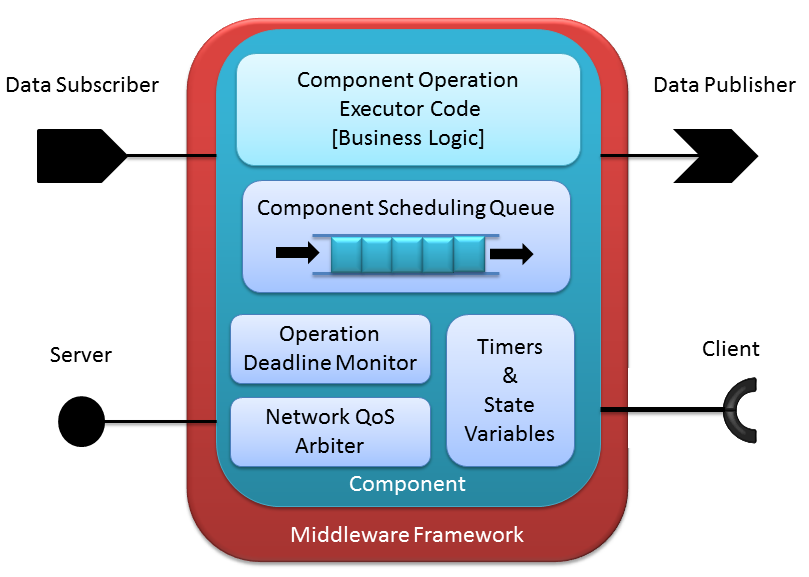
\includegraphics[width=0.85\textwidth]{figs/ros_component.png}
  \caption{Schematic representation of a software component.}
  \label{fig:component}
\end{figure}

From this component definition, we can define an application as a
grouping of components and a mapping between the ports of components:
\begin{equation}
  A = \{\{C\},\{M\}\}
\end{equation}

Where

\begin{itemize}
\item $\{C\}$ is the \emph{set} of components in the application
\item $\{M\}$ is the \emph{set} of \emph{mappings} between ports of
  the components in $\{C\}$, for instance connecting a subscriber of
  $C_x$ to a publisher of $C_y$, $M_{x,y} : C_x\{P_S\}\mapsto
  C_y\{P_P\}$.
\end{itemize}

And finally, an application's components are grouped into processes
and distributed onto the nodes of a system through a deployment
defined as a collection of nodes, processes, and a mapping from the
nodes to the processes:
\begin{equation}
  D = \{\{N\},\{U\},\{M\}\}
\end{equation}

Where

\begin{itemize}
\item $\{N\}$ is the \emph{set} of hardware \emph{nodes} in the system
\item $\{U\}$ is the \emph{set} of \emph{processes} defining the deployment,
  where a process is a collection of components
  $U=\{C\}\subseteq A\{\{C\}\}$.
\item $\{M\}$ is the \emph{set} of \emph{mappings} between processes and nodes
  in the system, e.g. $M_{U_1,N_1} : U_1\mapsto N_1$.
\end{itemize}

Note here that though the components are single threaded internally,
the application containing these components may run them in parallel,
e.g. by grouping them into a process or distributing them among the
hardware nodes of the system.  An example application and deployment
onto a system of nodes is shown in Figure~\ref{fig:cbse}.  Note that
multiple applications (shades of blue in this figure) may be deployed
simultaneously onto the same system and may even interact with each
other.  By using this component modeling framework and the associated
code generation tools we have developed, the application developer
needs only to provide the business-logic code for the application; the
rest of the middleware and component configuration code is
automatically provided by our library.

\begin{figure}[ht!]
  \centering
  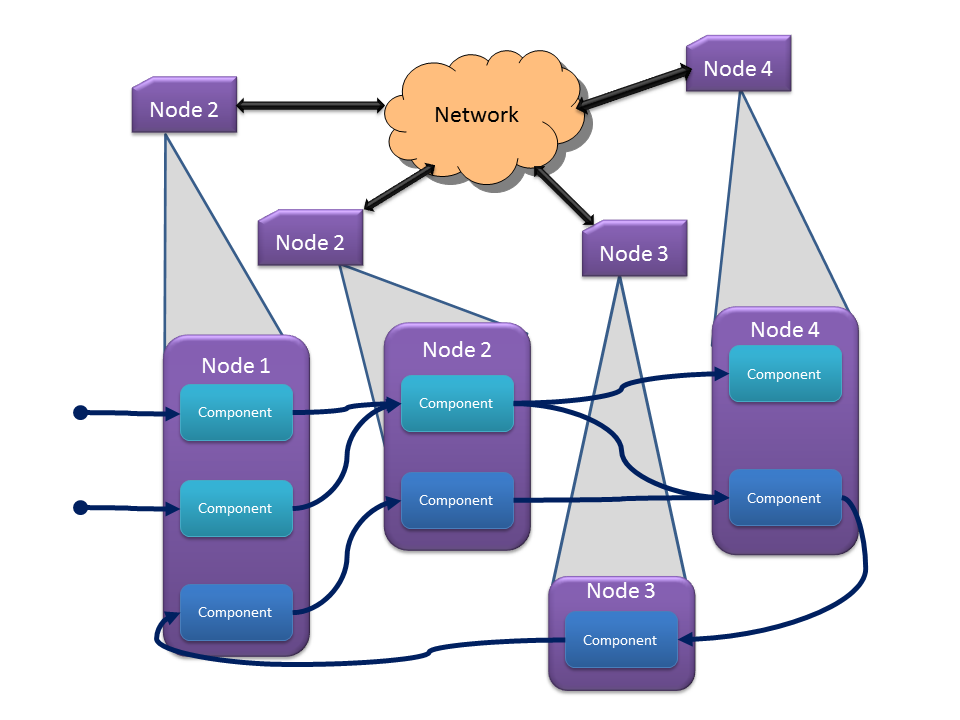
\includegraphics[width=0.85\textwidth]{../doc/src/images/results/cbse.png}
  \caption{Two example distributed CBSE applications deployed on a system with
    4 nodes.}
  \label{fig:cbse}
\end{figure}
   
To facilitate experimentation and testing of our analysis techniques,
we have developed network traffic production and consumption code
which produces or consumes traffic on a communications link according
to either a sender profile or receiver profile.  These profiles are
the same profiles used in the design-time analysis.  We integrated
this producer/consumer code into our component code-generators, which
generate component skeleton code and communications middleware glue
code based on our component model.  Both sender and receiver
automatically measure and record the network traffic for offline
analysis.

Since the sender middleware code is automatically measuring and
recording the output traffic from the application, we implemented
additional code which can optionally push-back to the application by
throwing and exception when the application is producing more data
than specified in its profile.  This push-back helps prevent a single
application from producing more data than the system was designed for
and flooding the network.  In the case that such a push-back occurs,
the application is notified and the data is not transmitted onto the
network.  Using this mechanism, a malicious or faulty application can
be prevented from flooding the network and degrading the service of
the network to other applications.

Similarly, since the receiver middleware code is automatically
measuring and recording the input traffic from each of its senders, we
implemented an additional communications channel which is used by the
sender and receiver middleware and allows out-of-band communication
which is invisible to the application.  This out-of-band channel
allows the sender to detect anomalies and inform the sender-side
middleware of such anomalies.  Further details about this capability
and uses are explained in Section~\ref{sec:ddos}.

The development of this producer/consumer/measurement code not only
helps with running experiments and data collection but also helps to
ensure model to system consistency.
  
\begin{figure}[ht!]
  \centering
  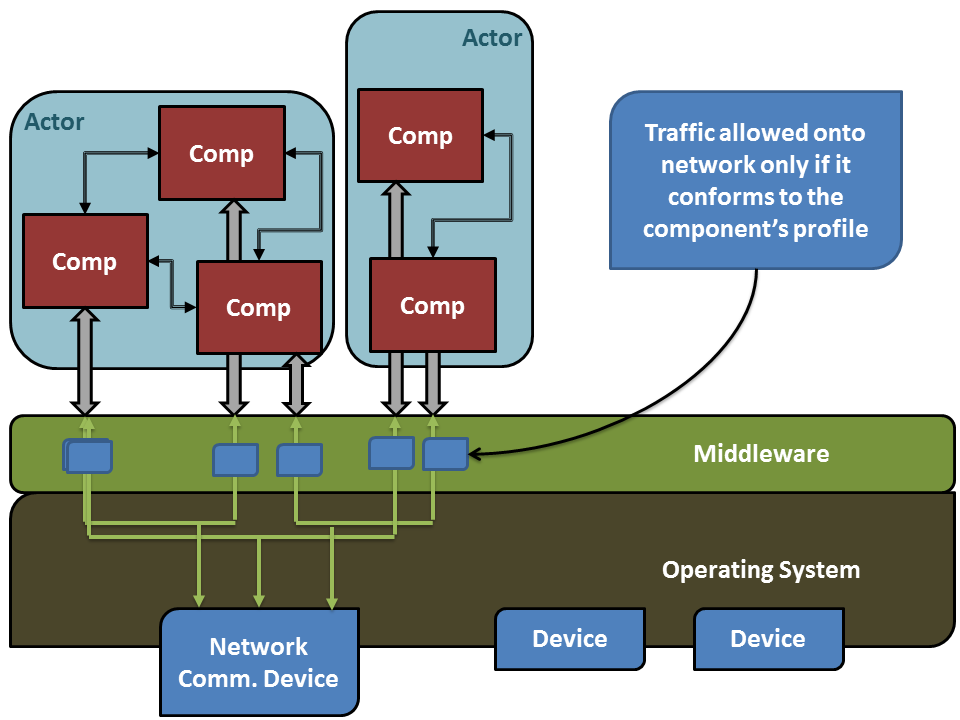
\includegraphics[width=0.85\textwidth]{../doc/src/images/results/app_layers.png}
  \caption{The structure of component-based applications and how their network
   traffic traverses the middleware and the OS stack.}
  \label{fig:sender}
\end{figure}

We have implemented profile-based traffic production/consumption and
traffic measurement into our code generators that we use with our
model-driven design software.  We developed this toolsuite to create
distributed component-based software which uses the Robot Operating
System (ROS)\cite{ros} as the communications middleware.  ROS provides
the capability for managing message passing, event triggering, and
timer triggering that we need for our software components.  For
publish/subscribe interactions between components, into the
publisher's generated code we add generic traffic producer code which
publishes traffic according to the sender profile.  Additionally,
these publish operations are configured to use a small wrapper
function which can measure the publish rate and can decide to throw a
\emph{profile exceeded} exception if the application attempts to send
too much data or if the receiver has pushed back to the sender
informing it to stop.  The sender-side middleware layer is shown in
Figure~\ref{fig:sender}.

This push back from the receiver occurs through the use of an
out-of-band (OOB) channel using UDP multicast, which receivers use to
inform specific senders that they are sending too much data to the
receivers (and possibly overflowing the receiver buffers).  This OOB
channel provides a mechanism by which the secure middleware layer can
protect the system from malicious or faulty applications.

Into the receiver code (for subscribers) we additionally generate a
receive buffer and receiver thread which pulls data from the buffer
according to the receiver profile.  In this scenario, the receiver has
a capacity with which it can handle incoming data, and it has a finite
buffer so it must use the OOB channel and measurements on the incoming
data stream to determine which senders to shut down to ensure its
buffer does not overflow.  When the buffer has had some time empty (so
that it's not in danger of running out of buffer space), the receiver
can use the OOB channel to inform the halted senders that it is
alright to send again.  The complete description of the OOB channel,
and the way the receiver limits the senders can be found in
Section~\ref{sec:ddos}.  An example of our traffic producer's accuracy
is shown in Figure~\ref{fig:generation}.  For the data in this figure,
each message was recorded as a tuple of $timestamp, message size$,
where the timestamp is the time at which the message was either sent
by the application.

\begin{figure}[ht!]
  %\centering
  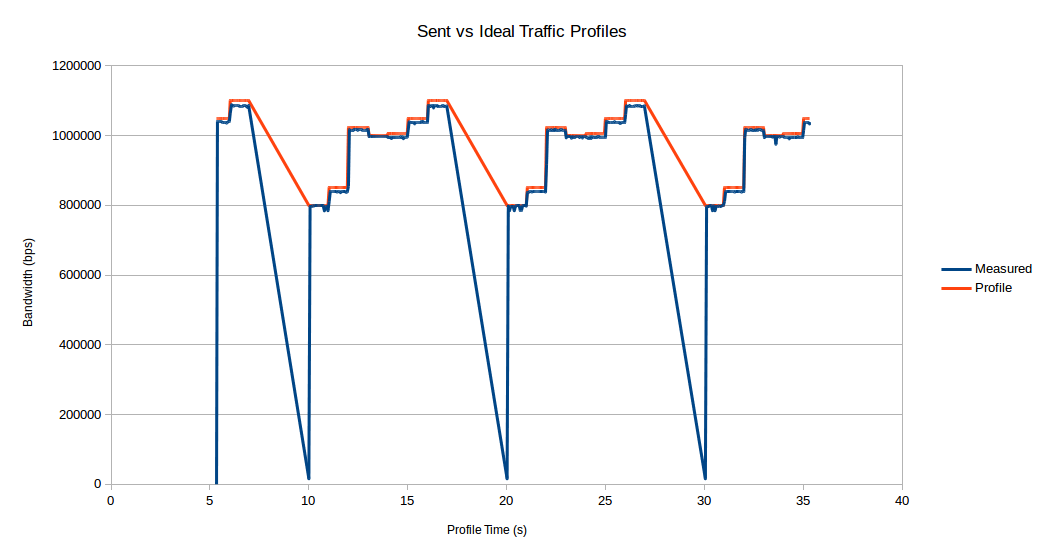
\includegraphics[width=1.1\textwidth]{../doc/src/images/results/traffic_generation.png}
  \caption{Demonstration of the accuracy with which our traffic
    producers follow the specified profile.}
  \label{fig:generation}
\end{figure}

\iffalse

\begin{definition}[Note:]
The measured bandwidth profile is calculated based on
recorded time series data of $[reception\_time,
message\_size]$, so the bandwidth drops to nearly 0
periodically since the $\Delta t$ is so large between
the messages.
\end{definition}

\begin{definition}[Note:]
Our original implementation of traffic producers performed
	  better since they did not utilize a middleware layer and
	  relied instead on simple point to point ipv6 connections.
	  However, that code was less useful for system analysis
	  because it could do nothing aside from traffic production
	  and measurement; our current implementation which generates
	  traffic production code into component code is more
	  versatile for several reasons:

          \begin{itemize}
	  \item The component-based code integrates directly into our development
	    toolsuite and deployment framework so it can be easily deployed on
	    our cluster.
	  \item Configuring different system topologies or component to host
	    mappings (deployments) is simpler and more robust, allowing us to
	    perform more and more varied experiments.
	  \item The traffic production code can be removed (or the code can be
	    regenerated without the option selected) and the rest of the
	    component-based and middleware code is still useful as an actual
	    application.
          \end{itemize}
\end{definition}

\fi

\newpage
%%%%%%%%%%%%%%%%%%%%%%%%%%%%%%%%%%%%%%%%%%%%%%%%%%%%%%%%%%%%%%%%%%%%%%%%%%%%%%%%%%%
%%%%%%%%%%%%%%%%%%%%%%%%%%%%%%%%%%%%%%%%%%%%%%%%%%%%%%%%%%%%%%%%%%%%%%%%%%%%%%%%%%%
%%%%%%%%%%%%%%%%%%%%%%%%%%%%%%%%%%%%%%%%%%%%%%%%%%%%%%%%%%%%%%%%%%%%%%%%%%%%%%%%%%%
%%%%%%%%%%%%%%%%%%%%%%%%%%%%%%%%%%%%%%%%%%%%%%%%%%%%%%%%%%%%%%%%%%%%%%%%%%%%%%%%%%%
%%%%%%%%%%%%%%%%%%%%%%%%%%%%%%%%%%%%%%%%%%%%%%%%%%%%%%%%%%%%%%%%%%%%%%%%%%%%%%%%%%%
\section{Distributed Denial of Service (DDoS) Detection}
\label{sec:ddos}

\subsection{Problem}
For distributed systems which must ensure resource availability and
system stability, a key aspect of the infrastructure is detection and
mitigation of faults or anomalies.  With respect to network resources,
an example is checking source and destination for communications to
enforce only authorized communication flows are present in the system.
However, software glitches or compromised applications can exceed
system resources that they have been allocated.  As described in the
previous section, higher-fidelity resource modeling and monitoring is
required to prevent such faults or compromises from propagating
throughout the system.  However, mitigating the propagation only
solves part of the problem; ideally the system should classify the
type of fault or anomaly and begin diagnostics to trace the
fault/anomaly back to its origin.  In this thesis we will address only
the problem of detecting and mitigating Distributed Denial of Service
attacks.  

Denial-of-Service (DoS)\cite{rfc4732} and Distributed DoS (DDoS) attacks
can take many forms, but are generally classified as excessive traffic
from a large amount of (possibly heterogeneous) sources targeted
towards a single point or a single group.  Such attacks are common to
machines on the internet, but can also become a hazard for machines on
private networks which become infected or inadvertently expose an
input path for external malicious data.

These private or semi-private systems must have mechanisms for
detecting and mitigating such attacks, and the combination of our
design-time analysis and run-time measurement, detection, and
mitigation tools provides a form for such capability.  The goal of
this work is for a receiver, which is being targeted for attack by a
set of senders, to determine which of the senders are behaving
anomalously and prevent them from sending any more data.  In this way,
a group of senders performing a DDoS attack can be mitigated by the
targeted receiver.  Towards this goal we make the following changes
outlined below to our modeling/analysis framework and implementation.

\subsection{Results}
Because these types of attacks come from systems for which the
application profiles may not be completely or fully known, we must
alter our modeling semantics such that we can model these types of
applications and the uncertainty surrounding their data rates.  

If we relax the constraint on the modeling semantics that all
sender profiles are absolute and the system behavior is completely
known at design-time, then we not only expand the scope of
applications that can be supported but also enable meaningful anomaly
detection.

Whereas previously, profiles modeled the exact $data\ rate$ as a
function of time that the application produced, we now alter the
definition to capture two parameters: $mean\ data\ rate$ ($\mu$) and
$max\ data\ rate$ ($MDR$), which again are both functions of time.
Just as before, these functions are constant-valued between successive
values of $t$ and are time-integrated to produce the $mean\ data$ and
$max\ data$ cumulative profiles as functions of time.  With this
specification, we no longer know exactly how much data an application
will produce at a given point in time, but instead are provided two
values by the developer: the $mean$ and $max$.

Now that we have these two profiles for the application, we could
simply analyze the $max$ data profile to determine buffer and latency
requirements, but this would end up wasting resources by allocating
memory and network resources of the system to the application even if
is not producing data at its \emph{max rate}.  Instead, we analyze the
system according to the $mean$ data profile to determine buffer
requirements and latency for the application in the system.  In doing
so, two buffer overflow risks are possible: 1) Sender-side buffer
overflow, and 2) Receiver-side buffer overflow.

We make the assumption that the application meters its sending to
prevent the first scenario, so that its data is not lost before making
it onto the network.  In this case, the sender can still send data at
a rate greater than the $mean$, but that rate is partially
governed by the capacity given to it by the node's network.

For the second case, we must ensure that there is no buffer overflow
on the receiver-side.  To enable this functionality, we must provide a
mechanism for the receiver to communicate with the sender.  This
push-back communication should travel through a channel outside the
communications channel that the application has access to, so that the
application, either maliciously or inadvertently, cannot disrupt this
push-back and in turn cause the receiver's buffer to overflow.  For
this reason, we add into the sender and receiver middleware an
out-of-band (OOB) channel that provides a communications layer between
all senders and receivers that is invisible to the application.  For
our component model and communications middleware, we have implemented
this OOB channel as a UDP multicast group.

Because the goal of this work is to meter only the senders which are
producing \emph{too much} data, we must define what too much data is.
Because we have developed these application profiles for analysis, and
these profiles describe the mean data rate, $\mu$, and the max data
rate, $MDR$, of the senders, they will be used to determine when a
sender is sending too much data.  In this paradigm, sender $S_i$ is
determined as behaving anomalously (i.e. sending too much data) if it
is sending data at a rate $DR_i > \mu_i$.  The assumption implicit in
this comparison is that the receiver, to be able to make this
comparison, has full knowledge of $\mu_i$, since $DR_i$ is calculable
on the receiver side.  If the receiver's buffer is filling up, it
looks through the the measured $DR_i$ (within a certain window of
time) for each of the senders it has been receiving data from, and
compares it against the sender's $\mu_i$.  If the comparison is
\emph{true}, it uses the OOB channel to push back to that specific
sender, informing the sender-side middleware to stop transmitting data
until the receiver has re-enabled that sender's transmission.  When
the receiver has emptied it's buffer enough it can then use the OOB
channel to re-enable any disabled senders.  The algorithm used by the
receiver to determine which senders to limit is shown in
Listing~\ref{lst:ddos_alg}, and has been integrated into our middleware.

\begin{listing}[ht!]
  \begin{minted}{python}
  receiver::limit_ddos( t_start, t_end )
  {
    for sender in senders
    {
      d_start = sender.received_data(t_start)
      d_end = sender.received_data(t_end)
      profile_d_start =
        sender.profile(t_start)
      profile_d_end =
        sender.profile(t_end)
      allowed_data = profile_d_end - profile_d_start
      actual_data = d_end - d_start
      if actual_data > allowed_data
      {
        sender.disable()
      }
    }
  }
  \end{minted}
  \caption{Algorithm used by receivers to determine which senders to
    limit.  The receiver only looks at the behavior of senders within
    the time window between $t_{start}$ and $t_{end}$, which is
    configurable.}
  \label{lst:ddos_alg}
\end{listing}


\begin{figure}[ht!]
  \centering
  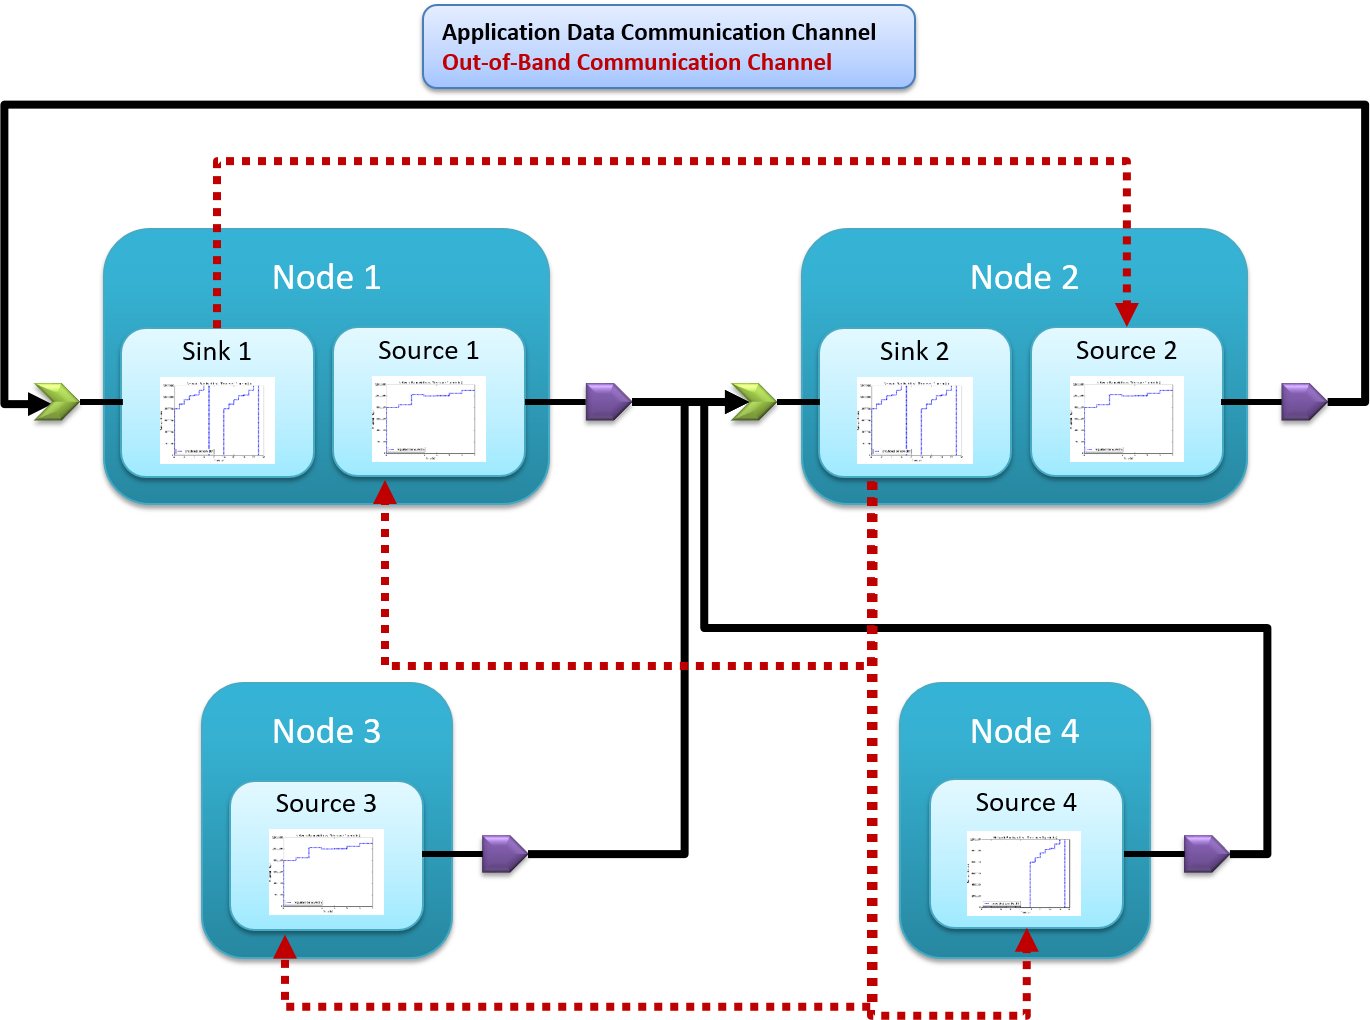
\includegraphics[width=0.85\textwidth]{../doc/src/images/results/example_setup.png}
  \caption{Nodes in an example network and how they communicate (using
    pub/sub).  The application communications are shown by the solid
    black arrows, and the out-of-band communications are shown by the
    red dotted arrows. }
  \label{fig:ddos}
\end{figure}

We have shown experimentally (for the system in Figure~\ref{fig:ddos})
that this measurement, detection, and mitigation strategy can protect
non-malicious clients from being denied service to a server by
malicious or faulty clients.  In this example, the client's data might
be lost if the server's buffer overflows.  Using the algorithm and
implementation described above, we show that the server is able to
keep its buffer from overflowing despite two of the three publishers
producing too much data.  In this scenario, the attackers would cause
dropped packets by producing data at a rate just less than their
$MDR$, which would require a server side buffer of 459424 bits.
However, the server detects that its buffer might overflow and that
the two malicious clients are producing too much data and it signals
for their middleware to prevent them from sending data.  In this way,
it maintains available buffer space (maximum buffer of 393792 bits) to
handle the good client's data and the good client is not denied
service.

\iffalse

for example, a receiver side buffer size of 400000 bits, which
would normally grow to 459424 bits because of excessive data pumps on
the sender sides, is kept to 393792 by utilizing this out-of-band
channel and secure middleware.

%%%%%%%%%%%%%%%%%%%%%%%%%%%%%%%%%%%%%%%%%%%%%%%%%%%%%%%%%%%%%%%%%%%%%%%%%%%%%%%%%%%
%%%%%%%%%%%%%%%%%%%%%%%%%%%%%%%%%%%%%%%%%%%%%%%%%%%%%%%%%%%%%%%%%%%%%%%%%%%%%%%%%%%
%%%%%%%%%%%%%%%%%%%%%%%%%%%%%%%%%%%%%%%%%%%%%%%%%%%%%%%%%%%%%%%%%%%%%%%%%%%%%%%%%%%
%%%%%%%%%%%%%%%%%%%%%%%%%%%%%%%%%%%%%%%%%%%%%%%%%%%%%%%%%%%%%%%%%%%%%%%%%%%%%%%%%%%
%%%%%%%%%%%%%%%%%%%%%%%%%%%%%%%%%%%%%%%%%%%%%%%%%%%%%%%%%%%%%%%%%%%%%%%%%%%%%%%%%%%
\section{Network Resource Monitoring and Management Integrated into Component-Based Middleware}
\label{sec:drems}

\subsection{Problem}
Distributed, deployed CPS require design-time assurances of system
stability and security.  These assurances guarantee that resources and
communications must have some protection against propagating software
faults or malicious actors.  One such avenue for fault or attack
propagation is the system's communications network.  Systems provide
the computational resources, hardware access, and communications
required for their applications.  For example, the satellite cluster
provides (1) distributed processors which are shared by the
applications, (2) data from the on-board sensors provided by each
satellite, and (3) a wireless communications network.  During
deployment, the system enforces resource utilization limits on the
applications, e.g. memory or disk space limitations, which must be
broad to account for whatever the applications may need to do over
their lifetime.  However, application resource limits which do not
incorporate temporal behavior (i.e. static limits) are inefficient
since they waste resources allocated to applications not using them.
Furthermore, these static resource limits do not provide tight bounds
on application behavior and may create avenues for fault or attack
propagation.  An example of such resource reservation schemes
backfiring is a Distributed Denial of Service (DDoS) attack, in which
many compromised applications produce slightly more network traffic
than usual (but still within their limits) to produce a combined
network traffic profile that can effectively take their target off of
the network.

\subsection{Contributions}
\begin{itemize}
	\item We integrated our network resource modeling techniques
          into a system and application analysis and development
          tool-suite. The tool verified that the system could provide
          all the network resources (which varied as a function of
          time) required by the applications.  The accuracy of the
          predictions was described in
          Section~\ref{sec:experimentalVerification}.
	\item Into the application's generated middleware interface
          code we integrated measurement, detection, and mitigation
          code which (1) measured the characteristics of the
          application's network traffic, (2) detected if the
          application's network traffic exceeded its profile that was
          provided during system analysis, and (3) blocked all traffic
          from leaving application-space (i.e. it did not get into
          kernel-space) which was detected as having exceeded the
          profile.  We showed that this management code allowed
          properly shaped traffic onto the network and blocked
          improperly shaped traffic.
\end{itemize}

%%%%%%%%%%%%%%%%%%%%%%%%%%%%%%%%%%%%%%%%%%%%%%%%%%%%%%%%%%%%%%%%%%%%%%%%%%%%%%%%%%%
%%%%%%%%%%%%%%%%%%%%%%%%%%%%%%%%%%%%%%%%%%%%%%%%%%%%%%%%%%%%%%%%%%%%%%%%%%%%%%%%%%%
%%%%%%%%%%%%%%%%%%%%%%%%%%%%%%%%%%%%%%%%%%%%%%%%%%%%%%%%%%%%%%%%%%%%%%%%%%%%%%%%%%%
%%%%%%%%%%%%%%%%%%%%%%%%%%%%%%%%%%%%%%%%%%%%%%%%%%%%%%%%%%%%%%%%%%%%%%%%%%%%%%%%%%%
%%%%%%%%%%%%%%%%%%%%%%%%%%%%%%%%%%%%%%%%%%%%%%%%%%%%%%%%%%%%%%%%%%%%%%%%%%%%%%%%%%%
\section{Network Application Fault/Anomaly Classification}
\label{sec:classification}

\begin{itemize}
	\item We will use our testbed to run distributed network tests
          to classify certain types of anomalies, e.g. DDoS attacks
          from compromised applications within the cluster.
	\item We will use the network resource utilization
          measurements gained from the tests to derive metrics which
          allow us to differentiate between classes of behavior,
          e.g. standard/stable application behavior vs. DDoS behavior.
	\item We will then use the classifications to show that the
          system can detect these types of attacks, mitigate their
          propagation, and report the attack to the system's manager.
\end{itemize}

\fi


%\chapter{Future Work}
\label{ch:future_work}

In this work we have described the beginning of precise, comprehensive
network system performance analysis and prediction.  However, we could
not possibly cover the modeling and analysis of all possible system
configurations, communication protocols, or interaction paradigms.
Furthermore, we have examined the affect certain system configuration
parameters or modeling choices have on our analysis techniques and
results, but such examination is not exhaustive.

Extending this work would focus on these areas in the following ways:

\begin{itemize}
  \item Moding and analysis support for more (commonly used)
    transmission protocols
  \item Relaxing modeling constraints and analyzing the affect of such
    relaxation on the predicted performance of the system
  \item Investigating run-time implementation alternatives and data
    analysis techniques
\end{itemize}

Towards the first area, a primary extension to the modeling framework
would be the support of retun-path communications and the impact they
have on the system.  Such modeling and analysis would allow for the
inclusion of TCP-based communications and could pave the way for
reactive system analysis using these techniques.  

Similarly, one of the model constraints which can be relaxed and
analyzed is the system-wide time-synchronization constraint.  If that
constraint is relaxed such that the nodes are known be re-synchronized
periodically with some predictable drift, then such behavior can be
directly analyzed similarly to the TDMA analysis.  From this
information, maximum deviations on the required buffer and delay can
be calculated, similarly to the deviations calculated for TDMA
systems.


\chapter{Conclusions}
\label{ch:conclusions}

We have described in this proposal the what aspects of Cyber-Physical
Systems(CPS) analysis, design, development, and integration we are
addressing.  We have provided descriptions of the relevant related
work in this area, covering both the design-time modeling, analysis,
and performance prediction for networked, distributed, CPS
applications and the run-time monitoring and management of application
and CPS network resources.

Subsequently, the completed research towards precise network
performance prediction, \shorttool/, was presented.  We showed how
different aspects of applications and systems could be analyzed,
culminating in the composition of multiple applications in a
distributed, statically routed system configuration.

Run-time network monitoring and anomaly detection mechanisms were
presented which used the modeling semantics from the design-time
techniques and showed how such models could be used for ensuring
quality of service (QoS) at run-time for distributed, networked
systems.

Finally, some areas of future work were presented which would extend
the capabilities of our techniques and would increase the domain over
which our analysis would be applicable.  



\begin{appendices}
  \chapter{Publications}
\label{ch:publications}

\section{Highly Selective Conference Papers}
\nobibliography*{}
\begin{itemize}
	\item \bibentry{ISIS_F6_ISORC_QOS:15}
\end{itemize}

\section{Other Conference and Workshop Papers}
\begin{itemize}
  
	\item \nobibentry{ISIS_F6_CYPHY:14}
	
	%\item \nobibentry{ISIS_F6_RTSS:13}\cite{ISIS_F6_RTSS:13}
	
	\item W. Emfinger, P. Kumar, A. Dubey, W. Otte, A. Gokhale, G. Karsai. DREMS: A Toolchain for the Rapid Application Development, Integration, and Deployment of Managed Distributed Real-time Embedded Systems. In \textit{Proceedings of the IEEE Real-Time Systems Symposium}, RTSS@Work 2013, Vancouver, Canada, 2013. IEEE
	
        \item \bibentry{rsp_2015_rosmod}

        \item \bibentry{rsp_2015_testbed}
	
	%\item \nobibentry{ISIS_F6_SMCIT:14}\cite{ISIS_F6_SMCIT:14}
	
	\item Pradhan S., W. Emfinger, A. Dubey, W. Otte, A. Coglio, D. Balasubramanian, A. Gokhale, G. Karsai. Establishing secure interactions across distributed applications in satellite clusters. In \textit{Proceedings of the IEEE International Conference on Space Mission Challenges for Information Technology}, SMC-IT, 2014, Laurel, MD, USA. IEEE
	
	%\item \nobibentry{ISIS_F6_FSW:13}\cite{ISIS_F6_FSW:13}
	
	\item Balasubramanian, D., W. Emfinger, P. S. Kumar, W. Otte, A. Dubey, and G. Karsai. An application development and deployment platform for satellite clusters.  In \textit { Proceedings of the Workshop on Spacecraft Flight Software}, 2013
	
	\item Balasubramanian, D., A. Dubey, W. R. Otte, W. Emfinger, P. Kumar, and G. Karsai. A Rapid Testing Framework for a Mobile Cloud Infrastructure.  In \textit{Proceedings of the IEEE International Symposium on Rapid System Prototyping}, RSP, 2014. IEEE
	
	\item Dubey, A., W. Emfinger, A. Gokhale, G. Karsai, W. R. Otte, J. Parsons, C. Szabo, A. Coglio, E. Smith, and P. Bose. A Software Platform for Fractionated Spacecraft. In \textit{Proceedings of the 2012 IEEE Aerospace Conference}, Big Sky, Montana, 03/2012. IEEE
	
	\item Levendovszky, T., A. Dubey, W. R. Otte, D. Balasubramanian, A. Coglio, S. Nyako, W. Emfinger, P. Kumar, A. Gokhale, and G. Karsai. DREMS: A Model-Driven Distributed Secure Information Architecture Platform for Managed Embedded Systems. In \textit{IEEE Software}, vol. 99: IEEE Computer Society, 2014. IEEE
	
\end{itemize}

\section{Submitted Papers - Awaiting Reviews}
\begin{itemize}
	\item W. Emfinger, P. Kumar, A. Dubey, G. Karsai. Towards Assurances in Self-Adaptive, Dynamic, Distributed Real-time Embedded Systems. In \textit{Software Engineering for Self-Adaptive Systems: Assurances}, 2015.
\end{itemize}


  \chapter{Configuration of Linux TC}
\label{ch:tc}

This chapter covers the specifics of how the routing, queuing, and
shaping of network traffic is configured and how this traffic passes
through the queues and shapers in the Linux Kernel before being
transmitted through the network interface.

We configure the system's static routes using the Linux's built-in
IPRoute\cite{linux_iproute} tool, which allows for the configuration
of the kernel's routing tables, network address translation (NAT), and
characteristics of the network interface such as the maximum transmit
unit (MTU).  For each node, a route is added to the routing table
specifying the next hop address as its gateway for each other node to
which it is not directly connected.  In this way, the packets in the
network will be routed using loose source-based routing where the
sender node does not know the full route that the packet will take,
but just forwards it to the next known location.

The system's priority-based network traffic queuing, network delay,
and network bandwidth capacity was configured using Linux's built-in
Traffic Control (TC)\cite{linux_tc} tool (which is part of IPRoute),
that allows for the configuration of hierarchical class-based traffic
scheduling, and traffic shaping.  We configured the output interfaces
on each node as a combination of two queuing disciplines (qdiscs): 1)
a network emulator (netem) which enforces the link delay, and 2) a
token-bucket filter (TBF) which enforces the rate control to enforce
the link's bandwidth profile.  On the routing node, we added an
additional priority qdisc (prio), with multiple priority queues.  We
configured TC to filter packets into these queues by matching packet
source IP address and destination IP address.  This filtering ensured
that the high priority flow's packets would be filtered into the
high-priority queue of the prio qdisc, while the lower priority flow's
packets would be filtered into the lower priority queue of the prio
qdisc.  All traffic out of the priority qdisc was fed into the TBF to
ensure that all traffic, regardless of priority, shared and was shaped
by the node's link capacity profile.  The configuration and function
of TC is shown in Figure~\ref{fig:tc_diagram}.

\begin{figure}[ht!]
  \centering
  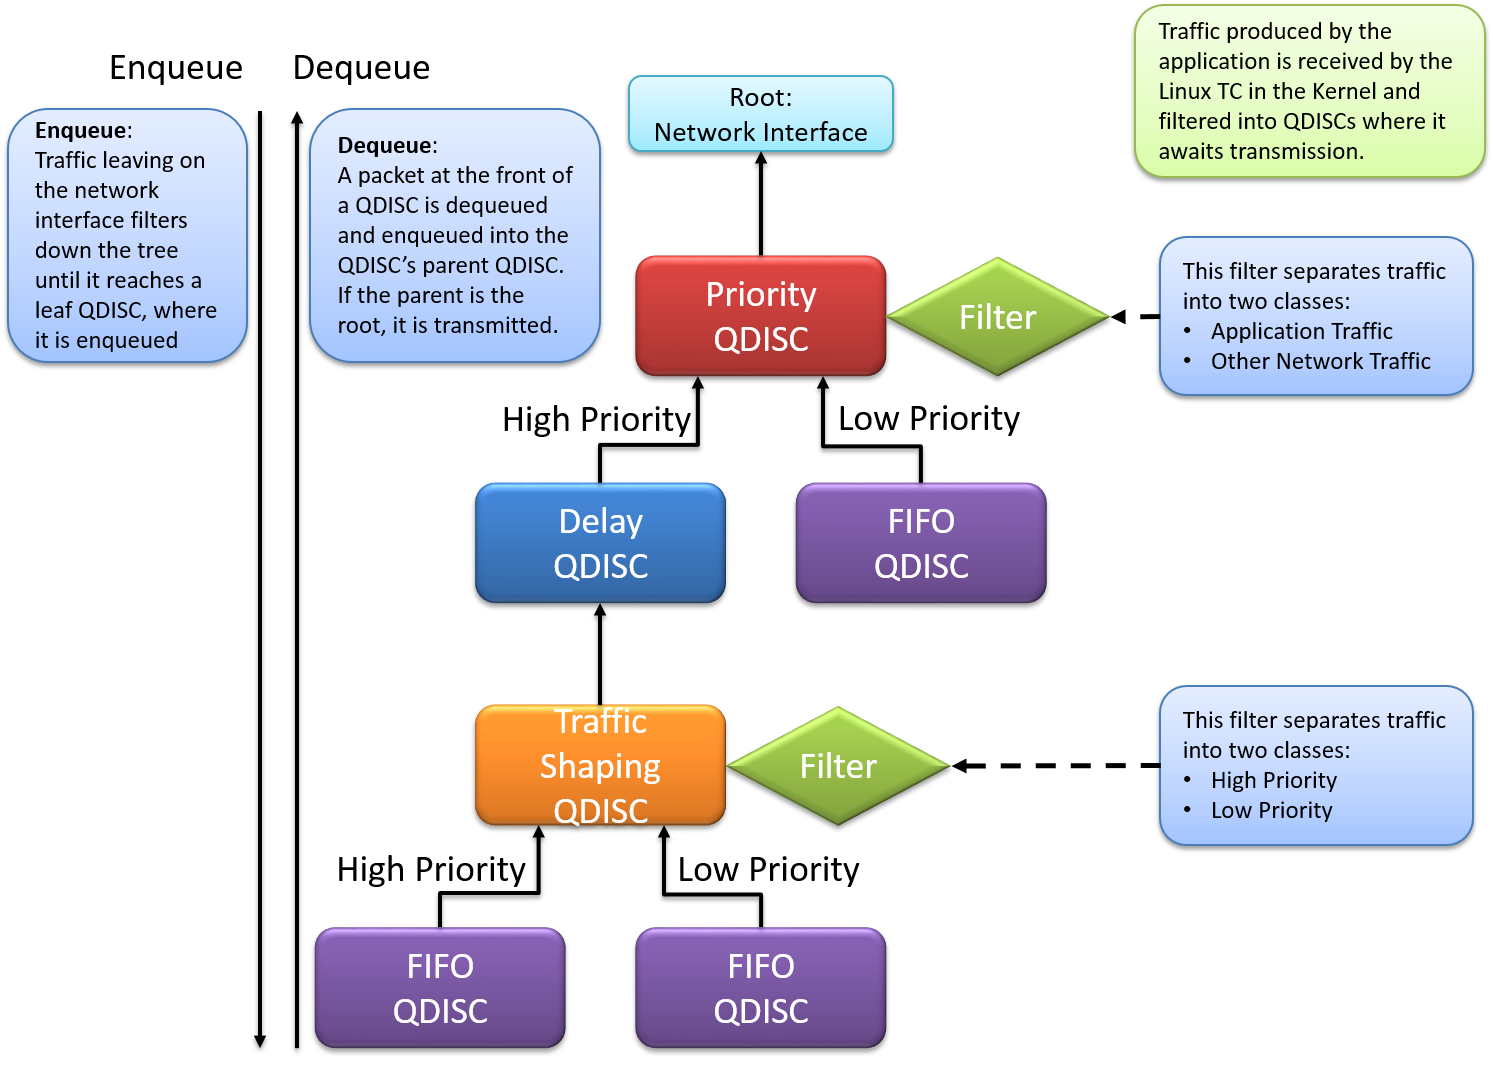
\includegraphics[width=\textwidth]{./figs/tc_diagram.png}
  \caption{Diagram illustrating the TC configuration used to implement
    priority flows, traffic shaping, and delay.}
  \label{fig:tc_diagram}
\end{figure}

\end{appendices}

%\balance
\bibliographystyle{abbrv}
\begin{spacing}{1}
\bibliography{./bibliography/f6}
\end{spacing}

\end{document}
